\documentclass[11pt,oneside]{book}
\usepackage{fontspec}
\usepackage{xeCJK}
\setmainfont{Latin Modern Roman}
\setCJKmainfont[ItalicFont={Noto Serif CJK TC},BoldItalicFont={Noto Serif CJK TC Bold}]{Noto Serif CJK TC}
\setCJKsansfont{Noto Sans CJK TC}
\setCJKmonofont{Noto Sans Mono CJK TC}
\newfontfamily\proseunicodefont{DejaVu Serif}
\usepackage[margin=1in]{geometry}
\usepackage{microtype}
\usepackage{amsmath,amssymb,amsthm,mathtools,bm}
\usepackage{graphicx}
\usepackage{adjustbox}
\usepackage{xcolor}
\usepackage{booktabs}
\usepackage{array}
\usepackage{longtable}
\usepackage{enumitem}
\usepackage{float}
\usepackage{caption}
\usepackage{hyperref}
\usepackage{fancyhdr}
\usepackage{tikz}
\usetikzlibrary{arrows.meta,positioning,calc,decorations.pathmorphing}

\hypersetup{
  colorlinks=true,
  linkcolor=blue!50!black,
  urlcolor=blue!50!black,
  citecolor=blue!50!black
}

\setlength{\parskip}{0.5em}
\setlength{\parindent}{0pt}
\setlist[itemize]{topsep=0.25em,itemsep=0.2em}
\setlist[enumerate]{topsep=0.25em,itemsep=0.2em}
\setlength{\headheight}{40pt}
\numberwithin{equation}{chapter}

\newtheorem{theorem}{定理}[chapter]
\newtheorem{proposition}[theorem]{命題}
\newtheorem{lemma}[theorem]{引理}
\newtheorem{corollary}[theorem]{推論}
\theoremstyle{definition}
\newtheorem{definition}[theorem]{定義}
\newtheorem{example}[theorem]{例}
\theoremstyle{remark}
\newtheorem{remark}[theorem]{註}

\providecommand{\ket}[1]{\left\lvert#1\right\rangle}
\providecommand{\bra}[1]{\left\langle#1\right\rvert}
\providecommand{\braket}[2]{\left\langle#1\,\middle|\,#2\right\rangle}
\providecommand{\expect}[1]{\left\langle#1\right\rangle}
\newcommand{\lectureoverview}[1]{\paragraph{概述。} #1}
\newenvironment{classroomqa}{%
  \par\medskip
  \begin{minipage}{0.96\textwidth}
}{%
  \end{minipage}
  \par\medskip
}
\newcommand{\audiencequestion}[1]{\noindent\textbf{聽眾提問。} #1\par\smallskip}
\newcommand{\lecturerresponse}[1]{\noindent\textbf{回答。} #1\par}
\newcommand{\lecturetimestamp}[1]{\footnote{講課時間： #1.}}
\newcommand{\lectureframe}[1]{\par\smallskip{\centering\footnotesize\itshape 講課畫面： #1.\par}}
\newcommand{\editorialnote}[1]{\footnote{編者說明： #1}}

\makeatletter
\newcommand{\course@headerfont}{\normalfont\small\itshape}
\newcommand{\course@pagefont}{\normalfont\small}
\newcommand{\course@headerraise}{14pt}
\newlength{\course@headerboxheight}
\setlength{\course@headerboxheight}{\dimexpr\headheight-\course@headerraise-9pt\relax}
\newcommand{\course@leftheadbox}[1]{%
  \raisebox{\course@headerraise}{%
    \parbox[t][\course@headerboxheight][t]{0.82\textwidth}{%
      \raggedright\course@headerfont\strut\MakeUppercase{#1}\strut%
    }%
  }%
}
\newcommand{\course@rightheadbox}[1]{%
  \raisebox{\course@headerraise}{%
    \parbox[t][\course@headerboxheight][t]{0.82\textwidth}{%
      \raggedleft\course@headerfont\strut\MakeUppercase{#1}\strut%
    }%
  }%
}
\renewcommand{\chaptermark}[1]{\markboth{\MakeUppercase{\chaptername\ \thechapter.\ #1}}{}}
\renewcommand{\sectionmark}[1]{\markright{\MakeUppercase{\thesection\hspace{0.4em}#1}}}
\fancyhf{}
\fancyhead[L]{\course@leftheadbox{\leftmark}}
\fancyhead[R]{\course@pagefont\thepage}
\renewcommand{\headrulewidth}{0.5pt}
\pagestyle{fancy}
\fancypagestyle{plain}{%
  \fancyhf{}
  \fancyhead[L]{\course@leftheadbox{\leftmark}}
  \fancyhead[R]{\course@pagefont\thepage}
  \renewcommand{\headrulewidth}{0.5pt}
}
\makeatother

\renewcommand{\contentsname}{目錄}
\renewcommand{\chaptername}{章}
\renewcommand{\figurename}{圖}
\renewcommand{\tablename}{表}
\renewcommand{\proofname}{證明}
\renewcommand{\bibname}{參考文獻}
\emergencystretch=2em
\pdfstringdefDisableCommands{\def\proseunicodefont{}}

\geometry{paperwidth=177.6mm,paperheight=252mm,left=16mm,right=16mm,
 top=18mm,bottom=18mm,includeheadfoot,headheight=28pt,headsep=7mm,footskip=9mm}
\usepackage{scrextend}
\changefontsizes[17pt]{12pt}
\raggedbottom
\renewenvironment{classroomqa}{\par\medskip\begingroup}{\par\endgroup\medskip}
\fancyhf{}
\setlength{\headwidth}{\textwidth}
\fancyhead[L]{\parbox{\textwidth}{\raggedright\fontsize{9}{11}\selectfont\nouppercase{\leftmark}}}
\fancyfoot[C]{\small\thepage}
\renewcommand{\headrulewidth}{0.3pt}
\fancypagestyle{plain}{\fancyhf{}\fancyfoot[C]{\small\thepage}\renewcommand{\headrulewidth}{0pt}}

\graphicspath{{../../../generated_course_notes/supplementary/string_theory/2010_fall_string_theory_and_m_theory/figures/}{../../../generated_course_notes/supplementary/string_theory/2010_fall_string_theory_and_m_theory/assets/}}
\begin{document}
\frontmatter
\hypersetup{pageanchor=false}
\begin{titlepage}
\hyphenpenalty=10000\exhyphenpenalty=10000
\thispagestyle{empty}
\begin{tikzpicture}[remember picture,overlay]
  \node[anchor=center,inner sep=0] at (current page.center) {%
    \includegraphics[height=\paperheight,keepaspectratio]{../../../generated_course_notes/supplementary/string_theory/2010_fall_string_theory_and_m_theory/assets/cover-art.png}%
  };
  \node[
    anchor=north west,
    align=left,
    text width=0.78\paperwidth,
    fill=white,
    fill opacity=0.9,
    rounded corners=8pt,
    inner xsep=10pt,
    inner ysep=8pt
  ] at ([xshift=0.08\paperwidth,yshift=-0.06\paperheight]current page.north west) {%
    {\fontsize{30}{33}\selectfont\bfseries\color{black!88} 弦理論與 M 理論\\[0.85em]}
    {\large\color{black!72} 繁體中文版 / 2010年秋季・弦理論與M理論}
  };
  \node[
    anchor=south west,
    align=left,
    text width=0.68\paperwidth,
    fill=white,
    fill opacity=0.82,
    text opacity=1,
    rounded corners=6pt,
    inner sep=12pt
  ] at ([xshift=0.08\paperwidth,yshift=0.08\paperheight]current page.south west) {%
    {\normalsize\color{black!78} 原講授：Leonard Susskind\\[0.35em]}
    {\small\color{black!72} 講義輔助版本：\href{https://lazying.art}{LazyingArt LLC} / \href{https://github.com/lachlanchen/Video2Book}{Video2Book}}
  };
\end{tikzpicture}
\mbox{}
\end{titlepage}
\hypersetup{pageanchor=true}

\clearpage
\chapter*{關於本講義}
這些經獨立編輯的配套講義，依據 Leonard Susskind 的講課內容整理而成。內容是根據機器轉錄稿、字幕及部分黑板畫面重建，再與現有的原始資料核對。這些講義並非 Susskind 教授的原稿，也未經他審閱或認可。

本版本由 \href{https://lazying.art}{LazyingArt LLC} 使用開源的 \href{https://github.com/lachlanchen/Video2Book}{Video2Book} 工作流程製作。機器轉錄稿另行提供，其中可能有語音辨識錯誤。編輯上的釐清及較重要的重建內容均以註腳標示。
\clearpage
\tableofcontents
\mainmatter
\chapter{從強子 Regge 軌跡到光錐弦}

\lectureoverview{弦理論最初並不是量子引力理論，而是為了理解強子的粒子譜與散射而發展出來的。筆直的 Regge 軌跡暗示強子是延展物體；{\proseunicodefont π}介子--{\proseunicodefont π}介子散射中的對偶性則暗示，兩個表面上不同的過程，其實是同一個曲面的兩種切片方式。我們將循著這些線索進入世界面圖像，把強子弦重新詮釋為 QCD 通量管，接著利用無限動量參考系推導開弦的橫向力學。核心結果是，有效內部哈密頓量量度的是質量平方。因此，在這種描述中，與\(L^2\)成正比的胡克定律能量，會轉變成與\(L\)成正比的靜止能量；這正是定張力弦的特徵行為。}

\section{弦理論的強子起源}

大約在1968--1970年，促使弦理論萌生的問題與質子、中子，尤其是介子有關。夸克模型當時已是受到認真看待的想法，但強子的夸克組成尚未以今日的標準由實驗確立。膠子在一般討論中的能見度更低。Nambu 曾提出相關的規範場想法，但量子色動力學的完整理論架構當時尚未形成。當時可供研究的素材，是強作用粒子出乎意料地豐富的粒子譜。

暫且不區分質子--中子，將這兩種狀態都稱為核子，是有用的做法。核子之外，還有自旋較大的較重態；再往上，則有自旋更大、質量也更高的態。Chew 和 Frautschi 將這些粒子族整理在一張圖上，縱軸為角動量，橫軸為質量平方。以當時的單位計，質子質量約為 1 BeV；這個單位如今稱為 GeV。

以\(\hbar\)為單位量度角動量。對重子族而言，無因次自旋值為半整數，

\begin{equation}
  J=\frac12,\frac32,\frac52,\ldots,
\end{equation}

而介子族的自旋則為整數。引人注目的經驗事實是，無論哪一族，以\(M^2\)為橫軸作圖時，各態都大致落在一條直線上。以現代記號可寫成

\begin{equation}
  J\simeq \alpha_0+\alpha' M^2,
  \label{eq:l01-regge-trajectory}
\end{equation}

其中\(\alpha_0\)是截距，\(\alpha'\)是 Regge 斜率。\editorialnote{本講強調觀測到的線性關係及其近乎普適的斜率。引入截距記號只是為了簡潔地表示這項關係；這些軌跡是根據經驗得到的近似結果。}

最初那條直線並不令人信服，因為當時已知的點只有兩個，而任意兩點都能決定一條直線。真正令人驚訝的是後來的發現：新發現的態仍持續落在同一條直線附近。介子軌跡也呈現相同的規律。{\proseunicodefont π}介子從\(J=0\)附近開始，在 GeV 尺度上質量很小；{\proseunicodefont ρ}介子從\(J=1\)開始；更高的激發態則繼續往上延伸。一個粒子族中可能出現五、六或七個態。更令人驚訝的是，不同重子與介子的軌跡幾乎互相平行。因此，角動量每增加一個量子，質量平方也大致增加相同的量：

\begin{equation}
  \Delta J=1
  \quad\Longrightarrow\quad
  \Delta M^2\simeq \frac{1}{\alpha'}.
  \label{eq:l01-regge-spacing}
\end{equation}

\begin{classroomqa}
\audiencequestion{不同的 Regge 軌跡彼此平行，代表什麼意思？\lecturetimestamp{00:09:32}}
\lecturerresponse{選取一個粒子族，將其中所有激發態畫在圖上，它們會落在一條直線上。再對另一個介子族或重子族重複這個做法。雖然截距不同，這些直線的斜率卻大致相同。因此，角動量增加相同的量，所對應的\(M^2\)增量也大致相同。這個共同斜率稱為普適 Regge 斜率。}
\end{classroomqa}

與一般延展物體的比較，說明了這種規律為何重要。籃球旋轉時會獲得轉動能量，但其軌跡是彎曲的，不是直線；而且角速度高到一定程度，球就會被撕裂。原子也有轉動激發態，但最終會被游離，軌跡也就到此為止。強子呈現的序列簡單得多；在當時可取得的資料範圍內，並未顯示這個序列即將終止。

這個粒子譜顯示，強子的行為不像點粒子。點粒子沒有可供旋轉或形變的空間結構。電子沒有觀測到高自旋內部態的序列，因此在目前的實驗界限內可視為點狀。相較之下，強子可以被加速旋轉。它的粒子譜暗示其具有複合結構，而自旋與質量的關係則暗示，角動量增加時，物體也會發生形變。

\section{{\proseunicodefont π}介子--{\proseunicodefont π}介子散射中的對偶性}

粒子譜學提供了一條線索，{\proseunicodefont π}介子--{\proseunicodefont π}介子散射則提供了另一條線索。兩個{\proseunicodefont π}介子可以結合成類似{\proseunicodefont ρ}介子的共振態，之後再以兩個{\proseunicodefont π}介子的形式出現。在傳統費曼圖中，這是湮滅後再產生的過程，通常稱為\(s\)道過程。將同一個基本圖旋轉過來，就得到交叉的\(t\)道過程；在這個過程中，{\proseunicodefont π}介子之間交換一個類似{\proseunicodefont ρ}介子的粒子。

{\proseunicodefont ρ}介子並非孤立存在。它屬於一個 Regge 粒子族，因此，若要保持一致，似乎就必須在兩個道中都納入{\proseunicodefont ρ}介子及其所有激發態夥伴。示意如下：

\begin{equation}
  \mathcal A(s,t)\simeq
  \sum_n \mathcal A^{(s)}_{\rho_n}(s,t),
  \qquad
  \mathcal A(s,t)\simeq
  \sum_n \mathcal A^{(t)}_{\rho_n}(s,t).
  \label{eq:l01-channel-sums}
\end{equation}

這些表示式並非兩種應直接相加的近似。數值研究發現，對湮滅道中的共振態序列求和，所得結果已大致等於交換道預期的貢獻。反過來，交換態序列也能重現共振態的描述。因此，若將兩個完整的態序列相加，似乎會把同一份物理效應計算兩次。一般的微擾計算會認為，既然有兩種圖，就必須兩者都納入；然而，強子散射振幅卻暗示，這兩種道的描述彼此對偶。

\begin{figure}[H]
  \centering
  \includegraphics[width=0.82\textwidth]{lecture_01_figure_01.png}
  \caption{這張板書將 Chew--Frautschi 圖與湮滅道及交叉道圖連在一起，呈現粒子譜與散射這兩條線索如何構成同一個問題。}
  \lectureframe{00:14:20}
  \label{fig:l01-regge-duality-board}
\end{figure}

同樣的關係也可以整理成一幅清楚的示意圖。第一個面板呈現線性粒子譜，另外兩個面板則表示同一散射振幅在不同道中的展開。

\begin{figure}[H]
  \centering
  \resizebox{\textwidth}{!}{%
  \begin{tikzpicture}[>=Latex,thick]
    \begin{scope}
      \draw[->] (0,0) -- (4.2,0) node[right] {$M^2$};
      \draw[->] (0,0) -- (0,3.4) node[above] {$J$};
      \draw[blue!65!black] (0.45,0.35) -- (3.55,2.95);
      \draw[orange!80!black] (0.75,0.20) -- (3.85,2.80);
      \foreach \x/\y in {0.65/0.52,1.35/1.10,2.05/1.69,2.75/2.27,3.45/2.86}
        \fill[blue!65!black] (\x,\y) circle (0.07);
      \foreach \x/\y in {0.95/0.37,1.65/0.95,2.35/1.54,3.05/2.12,3.75/2.71}
        \fill[orange!80!black] (\x,\y) circle (0.07);
      \node at (2.1,-0.55) {parallel Regge families};
    \end{scope}
    \begin{scope}[xshift=5.7cm]
      \draw[->] (-1.5,1.2) -- (-0.3,0.25);
      \draw[->] (-1.5,-1.2) -- (-0.3,-0.25);
      \draw[decorate,decoration={snake,amplitude=1.5pt,segment length=7pt}]
        (0,0.25) -- (0,-0.25);
      \draw[->] (0.3,0.25) -- (1.5,1.2);
      \draw[->] (0.3,-0.25) -- (1.5,-1.2);
      \node at (0,-1.75) {$s$-channel tower};
    \end{scope}
    \begin{scope}[xshift=10.5cm]
      \draw[->] (-1.5,1.2) -- (1.5,1.2);
      \draw[->] (-1.5,-1.2) -- (1.5,-1.2);
      \draw[decorate,decoration={snake,amplitude=1.5pt,segment length=7pt}]
        (0,0.95) -- (0,-0.95);
      \node at (0,-1.75) {$t$-channel tower};
    \end{scope}
  \end{tikzpicture}}
  \caption{平行的 Regge 粒子族，以及強子對偶所涉及的兩種道展開。}
  \label{fig:l01-regge-duality-redraw}
\end{figure}

\section{一個世界面，兩種切片方式}

自然的做法，是尋找一段可以用兩種方式解讀的幾何歷史。以夸克--反夸克對表示一個{\proseunicodefont π}介子，並令時間軸朝上。不要只畫一維的粒子線，而要填滿夸克軌跡所圍出的區域。對這段二維歷史作水平切片，可能會看到兩條入射弦結合，之後又分開。改用另一種切片方式，則會看到一條弦從一側交換到另一側。這兩種費曼圖道的圖像不再是彼此獨立的機制，而是同一個曲面的不同分解方式。

\begin{figure}[H]
  \centering
  \includegraphics[width=0.78\textwidth]{lecture_01_figure_02.png}
  \caption{板書上的夸克線拓撲。對同一段二維歷史作不同切片，便得到共振態與交換態兩種解讀。}
  \lectureframe{00:17:50}
  \label{fig:l01-worldsheet-topology-board}
\end{figure}

夸克與反夸克之間的區域帶來另一個想法。在某一固定時刻的切片中，除了兩個端點，還有某種結構填滿兩端之間的整段區間。這個物體是一維的，也就是一條弦。在相互作用過程中，弦會掃出一個二維曲面。

\begin{definition}
點粒子的時空歷史是一條\emph{世界線}。弦的時空歷史則是一個\emph{世界面}。某一瞬間的弦，是其世界面的一個空間切片。
\end{definition}

\begin{figure}[H]
  \centering
  \includegraphics[width=0.78\textwidth]{lecture_01_figure_03.png}
  \caption{板書中填滿端點軌跡之間的曲面。時間切片與曲面相交，形成一維的弦。}
  \lectureframe{00:19:15}
  \label{fig:l01-worldsheet-filled-board}
\end{figure}

\begin{figure}[H]
  \centering
  \begin{tikzpicture}[>=Latex,scale=0.95]
    \fill[blue!10]
      (-2.6,-2.3) .. controls (-1.0,-1.0) and (-1.0,-0.4) .. (-0.2,0)
      .. controls (-1.0,0.5) and (-1.0,1.0) .. (-2.6,2.3)
      -- (2.6,2.3)
      .. controls (1.0,1.0) and (1.0,0.5) .. (0.2,0)
      .. controls (1.0,-0.4) and (1.0,-1.0) .. (2.6,-2.3) -- cycle;
    \draw[blue!65!black]
      (-2.6,-2.3) .. controls (-1.0,-1.0) and (-1.0,-0.4) .. (-0.2,0)
      .. controls (-1.0,0.5) and (-1.0,1.0) .. (-2.6,2.3);
    \draw[blue!65!black]
      (2.6,-2.3) .. controls (1.0,-1.0) and (1.0,-0.4) .. (0.2,0)
      .. controls (1.0,0.5) and (1.0,1.0) .. (2.6,2.3);
    \draw[red!75!black,dashed] (-2.9,-1.15) -- (2.9,-1.15)
      node[right] {time slice};
    \draw[orange!80!black,dashed] (-1.55,-2.5) -- (1.55,2.5)
      node[above] {crossed slicing};
    \draw[->] (3.45,-1.7) -- (3.45,1.8) node[above] {time};
    \node[blue!65!black] at (0,-2.7) {one world sheet};
  \end{tikzpicture}
  \caption{世界面的清晰示意圖。對同一曲面作不同切片，可將它整理成不同的中間道描述。}
  \label{fig:l01-worldsheet-redraw}
\end{figure}

這種幾何重構是探索性的，並非從第一性原理推導出完整理論。不同的人以不同方式形成了早期的弦圖像。這個想法的優點在於，同一個延展物體可以同時解釋兩種觀測：弦可以旋轉並形變，而它的世界面則能編碼對偶的散射道。

\begin{classroomqa}
\audiencequestion{為什麼要引入弦狀的橋接結構，而不是讓夸克之間交換一個普通粒子？\lecturetimestamp{00:21:20}}
\lecturerresponse{在某一瞬間，存在的不只是局域化的交換粒子，還有一個夸克、一個反夸克，以及遍布兩者之間各處的結構。這種結構可能從根本上是連續的，也可能由大量組分密集排列而成，近似為連續體；早期的圖像並未決定是哪一種。重要的是，整段區間都被占據，而且觀測到的軌跡沒有顯示出像普通鞋帶那樣終止的跡象；普通鞋帶的兩端通常繫著重物。}
\end{classroomqa}

\begin{classroomqa}
\audiencequestion{標準模型能描述{\proseunicodefont π}介子散射嗎？
\lecturetimestamp{00:22:45}}
\lecturerresponse{可以，但是否適用取決於能量範圍。在低能下，標準模型透過 QCD 及其低能描述，能說明許多{\proseunicodefont π}介子散射現象。在較高能量下，整系列強子交換都會變得重要，直接計算也更困難；此時，以弦的方式整理問題可能更有用。}
\end{classroomqa}

\begin{classroomqa}
\audiencequestion{早期實驗是否證明 Regge 軌跡永不終止？\lecturetimestamp{00:23:37}}
\lecturerresponse{沒有。實驗只顯示，當時觀測到的序列尚未出現終點。據此推論軌跡可以無限延伸，是一種富有啟發性的外推，並非測得的無限延伸。}
\end{classroomqa}

\section{通量管與尺度的轉變}

現代 QCD 為早期的圖像提供了場論詮釋。夸克與反夸克是膠子場的相反源。在一般電動力學中，將異號電荷分開時，電通量會向側面擴散。場會隨距離增加而減弱，因此電荷之間的區域不會維持固定的橫向剖面。QCD 則是非線性的，其動力學可以將相關的色電通量限制在連接夸克與反夸克的狹窄管狀區域中。

\begin{figure}[H]
  \centering
  \includegraphics[width=0.78\textwidth]{lecture_01_figure_04.png}
  \caption{夸克與反夸克之間的場線呈現為狹窄的通量管，而非自由擴散的庫侖場。}
  \lectureframe{00:25:15}
  \label{fig:l01-qcd-flux-board}
\end{figure}

\begin{figure}[H]
  \centering
  \begin{tikzpicture}[>=Latex]
    \fill[orange!14,rounded corners=8pt] (-3.0,-0.55) rectangle (3.0,0.55);
    \draw[orange!80!black,thick,rounded corners=8pt]
      (-3.0,-0.55) rectangle (3.0,0.55);
    \fill[blue!70!black] (-3.35,0) circle (0.17);
    \fill[red!75!black] (3.35,0) circle (0.17);
    \node[below] at (-3.35,-0.22) {$q$};
    \node[below] at (3.35,-0.22) {$\bar q$};
    \foreach \y in {-0.30,0,0.30}
      \draw[->,orange!85!black] (-3.05,\y) -- (3.05,\y);
    \draw[<->] (-2.9,-1.05) -- (2.9,-1.05) node[midway,below] {$L$};
    \node at (0,0.92) {approximately fixed transverse profile};
  \end{tikzpicture}
  \caption{受禁閉的通量管伸長時不會擴散。單位長度能量固定，因而有\(E=TL\)。}
  \label{fig:l01-qcd-flux-redraw}
\end{figure}

粒子圖像與場圖像只是以不同方式描述同一件事。在場的描述中，端點分開時，通量管仍大致維持相同的場強與橫截面積。在組分圖像中，拉伸能量會在兩端之間形成更多膠子結構。普通橡皮筋中的分子數固定，因此分子間距會增加，直到材料斷裂。試想每當出現空隙時，就插入一個新分子。如此一來，橡皮筋變長時，沿帶的分子密度仍可維持固定。這就是膠子場所要表達的類比：通量管藉由增長而延展，不會逐漸變細直到斷裂。

\begin{classroomqa}
\audiencequestion{構成電子的弦也會由膠子構成嗎？\lecturetimestamp{00:28:08}}
\lecturerresponse{這並不能由此推得。強子弦是質子尺度上的 QCD 物體。假設存在、與量子引力相關的基本弦，則會位於小得多的普朗克尺度附近；此處並無證據顯示電子是由強子膠子弦構成。引人注目之處在於，相關的數學架構出現在這兩種尺度上，而非兩種物理物體彼此相同。}
\end{classroomqa}

將強子圖像發展成完整的交互作用弦理論，雖然很有前景，卻未能完全建立所期待的強子理論。這套數學模型一再包含一個自旋為二的無質量粒子。在強子理論中，這個態看來像是不受歡迎的預言；若將它視為引力理論的一部分，其量子數卻恰好符合引力子。Joel Scherk 和 John Schwarz 作出了關鍵性的重新詮釋：這套理論或許描述的是量子引力，而不是強子。強子應用與基本弦應用在物理上有所不同，儘管早期的強子問題引領人們走向這套數學架構。

\begin{classroomqa}
\audiencequestion{通量線如何從正端點延伸到負端點？\lecturetimestamp{00:31:46}}
\lecturerresponse{通量線離開一個源並進入另一個源，就像磁力線從條形磁鐵的北極延伸至南極。兩端相反的標記表示通量的方向；條形磁鐵也有兩個相反的磁極，不會有兩個北極。}
\end{classroomqa}

\begin{classroomqa}
\audiencequestion{弦是連續的還是離散的？
\lecturetimestamp{00:32:45}}
\lecturerresponse{量子理論使這種區分變得微妙。電磁場可以表示為連續場，同時也有離散的量子。同樣地，弦可以用連續的方式描述，而其激發態則是量子化的。應根據所探討的問題，選用適當的描述；兩種描述都可能成立。}
\end{classroomqa}

\begin{classroomqa}
\audiencequestion{若改變穿過世界面的時空切片角度，交線仍會是一條弦嗎？\lecturetimestamp{00:34:20}}
\lecturerresponse{會。改變同時性切片就是作洛倫茲變換。新的切片與曲面相交，得到的是一條處於不同運動狀態的弦。即使弦的質心靜止，弦的內部也不是完全靜止的；它仍可能振動。``靜止''只表示其質心靜止。}
\end{classroomqa}

\section{相對論能量的兩種展開}

直接以相對論方式描述延展且振動的物體並不容易。一種有用的策略，是找出一個參考系，使物體的相關運動呈現普通非相對論力學的形式。先從單一粒子開始。在非相對論情況下，可寫成

\begin{equation}
  E_{\mathrm{nr}}=\frac{\bm p^2}{2m}+B,
  \label{eq:l01-nonrel-energy}
\end{equation}

其中\(B\)是與整體動量無關的內能或束縛能。對多個互不作用的粒子而言，動能項與內能常數項都分別相加。由於運動取決於能量差，與狀態無關的加法常數通常可以省略。

精確的相對論能量為

\begin{equation}
  E=\sqrt{\bm p^2c^2+m^2c^4}.
  \label{eq:l01-rel-energy-c}
\end{equation}

\begin{figure}[H]
  \centering
  \includegraphics[width=0.76\textwidth]{lecture_01_figure_05.png}
  \caption{非相對論動能與精確的相對論平方根式；討論中已修正\(c\)的冪次。}
  \lectureframe{00:38:45}
  \label{fig:l01-relativistic-energy-board}
\end{figure}

\begin{classroomqa}
\audiencequestion{相對論公式中的冪次是否應為\(p^2c^2\)和\(m^2c^4\)，而非最初寫在黑板上的冪次？
\lecturetimestamp{00:39:12}}
\lecturerresponse{是。由量綱一致性可知，正確的表示式為\(E^2=p^2c^2+m^2c^4\)。推得非相對論極限後，我們會令\(c=1\)；但在此保留這些冪次，能讓展開過程更清楚。}
\end{classroomqa}

當\(p^2c^2\ll m^2c^4\)時，提出\(m^2c^4\)，並利用\(\sqrt{1+\epsilon}\simeq1+\epsilon/2\)：

\begin{align}
  E
  &=mc^2\sqrt{1+\frac{p^2}{m^2c^2}}
  \notag\\
  &\simeq mc^2+\frac{p^2}{2m}.
  \label{eq:l01-low-momentum-expansion}
\end{align}

\begin{figure}[H]
  \centering
  \includegraphics[width=0.76\textwidth]{lecture_01_figure_06.png}
  \caption{小動量展開，得到靜止能量加上熟悉的非相對論動能項。}
  \lectureframe{00:41:30}
  \label{fig:l01-low-momentum-board}
\end{figure}

這個近似要求的不只是質心運動緩慢。盒子可以緩慢移動，但其中的粒子仍可能以接近光速運動。在這種情況下，內部動力學依然是相對論性的。要達到一般的非相對論極限，所選參考系中的所有相關組成粒子都必須以低速運動。

還有另一個有用的極限。沿\(z\)軸對整個系統作洛倫茲推進，直到每個組成粒子都具有很大的正縱向動量\(P_{zi}\)。足夠大的推進會使任何原本向後運動的組成粒子也向前運動。橫向動量與靜止質量則保持不變：

\begin{equation}
  P_{zi}\gg |p_{xi}|,|p_{yi}|,m_i,
  \qquad
  p_{\perp i}^2=p_{xi}^2+p_{yi}^2,
\end{equation}

以下從此處起令\(c=1\)。對大的\(P_{zi}\)作展開，得到

\begin{align}
  E_i
  &=\sqrt{P_{zi}^2+p_{\perp i}^2+m_i^2}
  \notag\\
  &=P_{zi}\sqrt{1+\frac{p_{\perp i}^2+m_i^2}{P_{zi}^2}}
  \notag\\
  &\simeq P_{zi}
  +\frac{p_{\perp i}^2+m_i^2}{2P_{zi}}.
  \label{eq:l01-large-pz-one-particle}
\end{align}

\begin{figure}[H]
  \centering
  \includegraphics[width=0.76\textwidth]{lecture_01_figure_07.png}
  \caption{在大\(P_z\)下的平方根展開式，將橫向動量與質量視為小量。}
  \lectureframe{00:46:45}
  \label{fig:l01-large-pz-board}
\end{figure}

對多個組成粒子而言，

\begin{equation}
  E\simeq
  \sum_i P_{zi}
  +\sum_i\frac{p_{\perp i}^2}{2P_{zi}}
  +\sum_i\frac{m_i^2}{2P_{zi}}.
  \label{eq:l01-large-pz-sum}
\end{equation}

第一項是守恆的總縱向動量。它非常大，但只是固定的加法項。保留或減去這一項都不會改變任何能量差；同理，在哈密頓量中加上其他守恆量，也不會改變運動方程。因此，具有動力學效應的部分為

\begin{equation}
  \begin{aligned}
    H_{\perp}=E-P_z
    &\simeq
    \sum_i\left(
      \frac{p_{\perp i}^2}{2P_{zi}}
      +\frac{m_i^2}{2P_{zi}}
    \right),\\
    P_z&=\sum_iP_{zi}.
  \end{aligned}
  \label{eq:l01-transverse-hamiltonian}
\end{equation}

\begin{figure}[H]
  \centering
  \includegraphics[width=0.78\textwidth]{lecture_01_figure_08.png}
  \caption{多粒子能量分解為守恆的縱向動量、橫向動能，以及依賴質量的內部項。}
  \lectureframe{00:49:16}
  \label{fig:l01-energy-sum-board}
\end{figure}

\section{無限動量參考系}

前面討論的極限，過去稱為無限動量參考系；如今通常以光錐座標表述。從哈密頓量可以直接看出它的意義。在量子力學中，

\begin{equation}
  i\hbar\frac{\partial}{\partial t}\ket{\psi}=H\ket{\psi}.
  \label{eq:l01-time-evolution}
\end{equation}

\(H_{\perp}\)中的所有非平凡項都按\(1/P_z\)縮放。隨著推進增強，能量差縮小，變化也變得較慢。這就是時間膨脹。高度推進的放射性系統看起來衰變得較慢；觀測時間若按相同比例延長，就可以補償這種效應。動力學並未因此消失，只是其時間尺度改變了。

\begin{figure}[H]
  \centering
  \includegraphics[width=0.78\textwidth]{lecture_01_figure_09.png}
  \caption{板書將約化能量辨識為產生推進後系統緩慢時間演化的哈密頓量。}
  \lectureframe{00:52:57}
  \label{fig:l01-hamiltonian-board}
\end{figure}

橫向項恰好具有非相對論形式\(p^2/(2m)\)，但在此扮演質量角色的是\(P_z\)。這在物理上是合理的：縱向動量越大，粒子就越難被橫向偏轉，因此縱向動量相當於橫向慣性。項\(m_i^2/(2P_{zi})\)與二維運動狀態無關，因此扮演內能或束縛能的角色。於是，三個空間維度中的相對論運動，轉化為垂直於推進方向的兩個維度中呈現非相對論形式的運動。

這正是以簡單的質量與彈簧模型描述相對論弦所需的條件。這個模型並不假設弦在自己的靜止系中運動緩慢，而是採用橫向動力學具有所需非相對論結構的參考系。

\section{以珠子和彈簧構成的開弦}

取一條開弦，也就是有兩個端點的弦。之後或許會有物體連接在端點上，但目前只考慮弦本身。以位於橫向位置\(\bm X_i(t)=(X_i(t),Y_i(t))\)的珠子近似這條弦，並用相同的彈簧將珠子彼此連接。離散哈密頓量為

\begin{equation}
  H_N=\sum_{i=1}^{N}
  \left[
    \frac{\mu_N}{2}\dot{\bm X}_i^{\,2}
    +\frac{k_N}{2}
      \left(\bm X_{i+1}-\bm X_i\right)^2
  \right].
  \label{eq:l01-discrete-string}
\end{equation}

只有動能項的話，珠子會彼此飛散。讓它們連成一條弦的，是最近鄰珠子之間的胡克定律項。

\begin{figure}[H]
  \centering
  \includegraphics[width=0.75\textwidth]{lecture_01_figure_10.png}
  \caption{以兩個橫向座標表示開弦的第一幅珠子與彈簧示意圖。}
  \lectureframe{01:00:30}
  \label{fig:l01-bead-chain-board}
\end{figure}

\begin{figure}[H]
  \centering
  \begin{tikzpicture}[>=Latex]
    \foreach \x in {0,...,8} {
      \fill[blue!65!black] ({0.85*\x},0) circle (0.09);
    }
    \foreach \x in {0,...,7} {
      \draw[decorate,decoration={zigzag,segment length=4pt,amplitude=2pt}]
        ({0.85*\x+0.10},0) -- ({0.85*\x+0.75},0);
    }
    \draw[->] (3.4,0.15) -- (3.4,1.25) node[above] {$\bm X_i(t)$};
    \draw[<->] (0,-0.65) -- (6.8,-0.65)
      node[midway,below] {$0\leq\sigma\leq\pi$};
  \end{tikzpicture}
  \caption{開弦的離散化調節模型。在取連續極限之前，珠子質量與彈簧常數會隨間距縮放。}
  \label{fig:l01-bead-chain-redraw}
\end{figure}

\begin{figure}[H]
  \centering
  \includegraphics[width=0.78\textwidth]{lecture_01_figure_11.png}
  \caption{取連續極限之前，並列寫出的離散動能項與胡克定律項。}
  \lectureframe{01:01:30}
  \label{fig:l01-discrete-energy-board}
\end{figure}

珠子數目增加時，每顆珠子的質量\(\mu_N\)必須趨近於零，才能讓整條弦的慣性保持有限。同時，彈簧常數\(k_N\)必須增大。相較於同種材料的小段橡膠，長條橡膠更容易拉長固定的量；因此，若要使連續材料的性質保持不變，距離更近的相鄰點就必須以更大的勁度連接。

引入沿著弦的座標\(\sigma\)。其取值範圍只是約定。選擇

\begin{equation}
  0\leq\sigma\leq\pi
\end{equation}

很方便，因為之後可以用從\(0\)到\(2\pi\)的參數來描述閉弦。求和會轉為積分，最近鄰差分則會轉為導數：

\begin{equation}
  \sum_i\longrightarrow\int_0^\pi d\sigma,
  \qquad
  \bm X_{i+1}-\bm X_i
  \longrightarrow
  \partial_\sigma\bm X.
  \label{eq:l01-continuum-replacements}
\end{equation}

將依賴間距的常數吸收到\(t\)、\(\sigma\)與\(\bm X\)的正規化中後，連續哈密頓量具有以下形式

\begin{equation}
  H_{\mathrm{string}}=
  \frac12\int_0^\pi d\sigma
  \left[
    \left(\partial_t\bm X\right)^2
    +\left(\partial_\sigma\bm X\right)^2
  \right].
  \label{eq:l01-continuum-hamiltonian}
\end{equation}

\begin{figure}[H]
  \centering
  \includegraphics[width=0.78\textwidth]{lecture_01_figure_12.png}
  \caption{板書展示了從珠子求和轉為\(\int_0^\pi d\sigma\)的過程，其中最近鄰差分以\(\partial_\sigma\bm X\)取代。}
  \lectureframe{01:05:00}
  \label{fig:l01-continuum-board}
\end{figure}

第一項是兩個橫向方向的動能，第二項量度弦的拉伸。由於這是哈密頓量，兩項的符號都是正的；在拉格朗日量中，勢能項則會帶負號。確切係數取決於所採用的約定，此處尚未確定；此處重要的是動能與拉伸項並存的結構。

將質心運動與相對運動分開。所有位置同時平移相同的量，會讓物體整體移動；振盪、彎曲與相對拉伸則是內部運動。即使內部組成部分彼此運動，質子、原子或其他複合物體仍可稱為粒子。弦在這方面並無不同。

\section{為什麼哈密頓量量度的是質量平方}

對緩慢運動的物體而言，靜止能量與其質量成正比。然而，在無限動量的描述中，內部貢獻表現為\(M^2/(2P_z)\)。固定共同的縱向動量及其所伴隨的時間尺度變換後，弦的內部哈密頓量便與整個物體的不變質量平方成正比：

\begin{equation}
  H_{\mathrm{int}}\propto M^2.
  \label{eq:l01-hint-mass-squared}
\end{equation}

\editorialnote{更明確地說，光錐運動學給出形式如\(M^2=2P^+P^- - \bm P_\perp^2\)的不變關係。在質心的橫向參考系中，並固定\(P^+\)時，光錐哈密頓量\(P^-\)因此與\(M^2\)成正比。本講省略這些正規化細節，只保留論證所需的比例關係。}

\begin{figure}[H]
  \centering
  \includegraphics[width=0.76\textwidth]{lecture_01_figure_13.png}
  \caption{板書將弦的內部能量與完整弦態的質量平方連結起來。}
  \lectureframe{01:10:30}
  \label{fig:l01-mass-squared-board}
\end{figure}

振動弦是由耦合振子構成的系統。完整的量子化留待之後討論，但重要的粒子譜特徵已經顯現。諧振子的能量以離散階梯上升。由於這些內部能量會貢獻至\(M^2\)，弦的激發態自然會使質量平方呈現離散的階梯。這正是開頭 Regge 圖所揭示的結構。

\begin{classroomqa}
\audiencequestion{\(M\)是整條弦的質量嗎？若質量加倍，相應的\(M^2\)貢獻會變成四倍嗎？
\lecturetimestamp{01:12:10}}
\lecturerresponse{是。\(M\)是完整弦態的靜止質量，其中包括振動、拉伸與所有其他內部貢獻。有效的推進系哈密頓量與\(M^2\)成正比，因此質量加倍的態，其質量平方值會變成四倍。}
\end{classroomqa}

\begin{classroomqa}
\audiencequestion{這種描述如何能涵蓋靜止質量為零的光子？\lecturetimestamp{01:12:52}}
\lecturerresponse{無質量態對應於\(M=0\)。正的振子貢獻如何組合成這種態，是量子化理論中的重要問題，並非此處的經典模型所能解決。在目前的討論中，\(M\)僅表示總靜止質量，且尚未引入量子力學。}
\end{classroomqa}

現在將一條靜止的弦均勻拉伸至物理長度 \(L\)。動能項消失；在長度為 \(\pi\) 的參數區間內，

\begin{equation}
  \left|\partial_\sigma\bm X\right|\simeq\frac{L}{\pi}.
\end{equation}

因此，

\begin{align}
  H_{\mathrm{stretch}}
  &\propto
  \int_0^\pi d\sigma
    \left(\partial_\sigma\bm X\right)^2
  \notag\\
  &\simeq
  \pi\left(\frac{L}{\pi}\right)^2
  \propto L^2.
  \label{eq:l01-hooke-l2}
\end{align}

\begin{figure}[H]
  \centering
  \includegraphics[width=0.76\textwidth]{lecture_01_figure_14.png}
  \caption{用來推知 \(H_{\mathrm{stretch}}\propto L^2\)，進而推知 \(M\propto L\) 的均勻拉伸構型。}
  \lectureframe{01:15:30}
  \label{fig:l01-length-relation-board}
\end{figure}

這是有效橫向力學中的胡克定律行為。但左側的量正比於 \(M^2\)，而非 \(M\)。因此，

\begin{equation}
  M^2\propto L^2,
  \qquad
  M\propto L.
  \label{eq:l01-mass-length}
\end{equation}

在靜止系中，能量為 \(E_{\mathrm{rest}}=M\)，單位制取 \(c=1\)。將比例常數記為弦張力 \(T\)，

\begin{equation}
  E_{\mathrm{rest}}=TL.
  \label{eq:l01-string-tension}
\end{equation}

結果與通量管的圖像相符。均勻的電場或磁場具有均勻的能量密度。若其通量被限制在截面固定的管中，每增加一單位長度，能量就會等量增加。等價地，在組成成分的圖像中，每個新開出的間隙都填入新的自由度，因此每單位長度的能量固定不變。弦張力就是這個單位長度能量。

這個結論是間接得出的。它並非聲稱，任意一條被加速至相對論速度的橡皮筋都會自動具有 \(E=TL\)。論證先從大幅洛倫茲變換後得到的橫向非相對論描述出發，將其內部能量認定為 \(M^2\)，然後才把結果轉換回靜止系能量。

\section{同一物體在兩個參考系中的描述}

\(M\)和 \(M^2\) 的區別很容易混淆，因此值得將兩種展開並列比較。取 \(c=1\)，

\begin{align}
  E&=\sqrt{p^2+M^2}
  \simeq M+\frac{p^2}{2M},
  &&p\ll M,
  \label{eq:l01-rest-expansion-again}\\
  E&=\sqrt{P_z^2+M^2}
  \simeq P_z+\frac{M^2}{2P_z},
  &&P_z\gg M.
  \label{eq:l01-boost-expansion-again}
\end{align}

\begin{figure}[H]
  \centering
  \includegraphics[width=0.74\textwidth]{lecture_01_figure_15.png}
  \caption{分隔處之後再次列出的小動量展開；其中內部靜止能量視為 \(M\)。}
  \lectureframe{01:28:00}
  \label{fig:l01-rest-expansion-board-again}
\end{figure}

\begin{figure}[H]
  \centering
  \includegraphics[width=0.74\textwidth]{lecture_01_figure_16.png}
  \caption{互補的大動量展開；其中剩餘能量正比於 \(M^2/(2P_z)\)。}
  \lectureframe{01:31:00}
  \label{fig:l01-boost-expansion-board-again}
\end{figure}

第一種展開將靜止能量等同於質量，並將普通慣性視為 \(M\)。在第二種展開中，守恆的 \(P_z\) 項被分離出去，橫向慣性為 \(P_z\)，內部能量則以 \(M^2/(2P_z)\) 表示。無論在哪個參考系中，質量都與弦長成正比。改變的是哪個質量函數會作為剩餘哈密頓量出現。

\begin{classroomqa}
\audiencequestion{洛倫茲變換不應改變物理。為什麼經過洛倫茲變換的弦看起來遵循不同的能量定律？
\lecturetimestamp{01:25:35}}
\lecturerresponse{它遵循的物理並沒有不同。在兩種描述中，\(M\propto L\) 且 \(M^2\propto L^2\)。在靜止系中，相關能量是 \(M\)；經過大幅洛倫茲變換後，守恆的 \(P_z\) 被分離出去，剩餘哈密頓量則正比於 \(M^2\)。洛倫茲變換改變的是方便使用的描述，而非不變的質量--長度關係。}
\end{classroomqa}

\section{超導體禁閉模型}

超導體會排斥其內部的磁場。若在材料變成超導體之前，磁通量已被困在足夠狹窄的通道中，磁通量便無法向側面擴散，而會被限制在一條管狀區域內。一個有用的思想實驗是：在常態樣品上鑽一個窄孔，將一根長條磁鐵穿過孔洞，冷卻樣品，再抽出磁鐵。這種構造只是示意，並非可實際操作的實驗室方案。其目的是隔離出一條磁通線，使其場強與能量密度沿線長方向近似均勻。

\begin{figure}[H]
  \centering
  \includegraphics[width=0.76\textwidth]{lecture_01_figure_17.png}
  \caption{超導體中的磁通線構造，以及相應的單極子--反單極子禁閉圖像。}
  \lectureframe{01:35:30}
  \label{fig:l01-superconductor-board}
\end{figure}

再設想一個思想實驗：假設可以將一個磁單極子和一個反單極子置於超導介質中，並將兩者分開。它們之間的磁通量會被擠壓成一條管狀區域。由於管狀區域每單位長度的能量都相同，

\begin{equation}
  V(R)=T_{\mathrm{flux}}R.
  \label{eq:l01-linear-confinement}
\end{equation}

力 \(F=-dV/dR\) 的大小為定值。將這對粒子拉得越遠，所需能量越高，因此兩者會受到禁閉。這正是夸克在強子中所需具備的行為。

\begin{figure}[H]
  \centering
  \begin{tikzpicture}[>=Latex]
    \fill[blue!8,rounded corners=5pt] (-4,-1.35) rectangle (4,1.35);
    \node[blue!55!black] at (0,1.65) {superconducting medium};
    \fill[red!75!black] (-2.8,0) circle (0.17);
    \fill[blue!70!black] (2.8,0) circle (0.17);
    \node[below] at (-2.8,-0.22) {monopole};
    \node[below] at (2.8,-0.22) {antimonopole};
    \fill[orange!18,rounded corners=7pt] (-2.65,-0.42) rectangle (2.65,0.42);
    \draw[orange!85!black,thick,rounded corners=7pt]
      (-2.65,-0.42) rectangle (2.65,0.42);
    \foreach \y in {-0.22,0,0.22}
      \draw[->,orange!85!black] (-2.55,\y) -- (2.55,\y);
    \draw[<->] (-2.8,-1.00) -- (2.8,-1.00) node[midway,below] {$R$};
  \end{tikzpicture}
  \caption{磁通禁閉形成均勻的管狀區域，並導致線性位能 \(V(R)=T_{\mathrm{flux}}R\)。}
  \label{fig:l01-superconductor-redraw}
\end{figure}

\begin{classroomqa}
\audiencequestion{在強子中，什麼扮演超導介質的角色？\lecturetimestamp{01:36:57}}
\lecturerresponse{這個類比將電與磁的角色對調。一般超導凝聚體帶有電荷，會禁閉磁通量。在量子色動力學（QCD）的對偶超導體圖像中，色磁性物體的凝聚體會禁閉夸克的色電荷。這類物體不會以孤立粒子的形式出現，因為在這個描述中，它們已凝聚於真空之中。}
\end{classroomqa}

\editorialnote{對偶超導體描述是一種頗具影響力的禁閉機制，此處沿用講座中的歷史性說法。應將它視為描述 QCD 真空的物理圖像，而非從第一原理完整推導禁閉的結果。}

\begin{classroomqa}
\audiencequestion{能量與長度成正比，對任何變得高度相對論性的普通弦來說，都是普遍規則嗎？\lecturetimestamp{01:38:10}}
\lecturerresponse{不是。首先必須有一套描述該材料且自洽的相對論理論，而其行為會取決於具體細節。能量隨長度線性增加，只是特定構型的性質：其密度在延展時維持不變，或其通量受到限制而無法向橫向擴散。將它拉開，會產生更多組成成分，或增加均勻充滿場的長度，而不只是增加一組固定分子彼此間的距離。}
\end{classroomqa}

\section{橫向自由度與粒子的大小}

光錐構造直接以弦的橫向座標描述弦。每個橫向振子都沒有一個可獨立指定的縱向振子與之對應。直接描述的空間維度少一個，是這套形式體系的顯著特徵之一；不過，完整理論仍須滿足洛倫茲不變性。

\begin{classroomqa}
\audiencequestion{沿著 \(z\) 方向的剩餘運動會如何處理？
\lecturetimestamp{01:40:10}}
\lecturerresponse{在光錐描述中，縱向運動不作為獨立自由度引入。物理振盪以橫向自由度描述，而縱向資訊則由約束條件決定。這種精簡的做法，在觀念上與引力系統或許能以少一個直接維度描述的想法相關，不過此處並未推導兩者之間的關聯。}
\end{classroomqa}

\begin{classroomqa}
\audiencequestion{雷吉圖上目前實際已知多少個點？
\lecturetimestamp{01:41:15}}
\lecturerresponse{確切的最大值依粒子家族而異，粗略來說約有七個。這些序列並非實驗上無窮無盡。重點是，已知的點沒有呈現普通宏觀材料常見的明顯失效或斷裂終點。}
\end{classroomqa}

強子現象學提供了歷史上的研究動機，但數學弦理論不必在每個細節上都重現強子。形式體系建立之後，接下來要問的是它實際描述什麼。無質量自旋二態及其他性質，顯示它更自然地指向引力。

強子與電子表面上的差異，可以用剛體轉動的能量加以量化：

\begin{equation}
  E_{\mathrm{rot}}=\frac{J^2}{2I},
  \qquad
  I\sim MR^2.
  \label{eq:l01-rotational-energy}
\end{equation}

角動量是量子化的。將 \(J^2\) 概略寫成 \(\hbar^2 n^2\)，第一個轉動能階差的量級為

\begin{equation}
  \Delta E_{0\to1}\sim\frac{\hbar^2}{2I}.
  \label{eq:l01-first-rotational-step}
\end{equation}

\begin{figure}[H]
  \centering
  \includegraphics[width=0.76\textwidth]{lecture_01_figure_18.png}
  \caption{第一個轉動激發的轉動慣量估算：\(\Delta E\sim\hbar^2/(2I)\)。}
  \lectureframe{01:44:00}
  \label{fig:l01-rotational-board}
\end{figure}

在質量固定時，半徑越小，轉動慣量就越小，激發能量也越高。相對於自身內部動力學的尺度，強子相當大，因此一次轉動激發約需一 GeV，在粒子碰撞中可達到。若電子具有任何空間子結構，實驗限制顯示其尺度遠小於強子的尺度，轉動激發所需的能量也會遠超現有可達範圍。籃球則處於另一極端：它的轉動慣量極大，以致一個角動量量子所需的能量小到無法察覺。原子的轉動或軌道能階躍遷則介於兩個極端之間，通常約為電子伏特的量級。

\begin{classroomqa}
\audiencequestion{看似基本粒子的電子，是否仍可能具有空間結構與轉動激發？\lecturetimestamp{01:42:04}}
\lecturerresponse{這些特徵只有可能出現在極高能量下，因而尚未被發現。一個單位角動量所需的能量按 \(1/I\) 縮放，而 \(I\sim MR^2\)。因此，半徑極小會使第一個激發態在質量平方圖上遠離目前可見的範圍。尚未觀察到電子激發，表示電子可能是點狀粒子，也可能是其複合尺度遠小於現有實驗所能解析的尺度。}
\end{classroomqa}

現在可以從動力學角度理解開篇的雷吉圖。強子是延展物體，因此會呈現可達到的轉動與振動態。其質量平方譜中的等間距步進，是振子哈密頓量對應於 \(M^2\) 時所預期的特徵。能量隨長度近似線性增加，則是張力固定的通量管所具有的特徵。光譜學、散射對偶性、世界面幾何與光錐力學，是描述同一核心概念的四種方式：一種延展的相對論物體，其自然的內部變數是質量平方。
\chapter{從邊界條件到開弦譜}

\lectureoverview{我們的目標是將開弦量子化，並判斷它的量子態是否稱得上粒子。這條路徑雖然初等，卻不容馬虎。我們先準備在 \(0\leq\sigma\leq\pi\) 上對函數進行微積分與傅立葉分析。接著，我們以譜判據取代點狀性來判斷粒子行為，回顧橫向動力學呈現非相對論形式的無限動量描述，並以一串輕質量與剛性彈簧建構弦。連續弦是具有自由端點的波動系統。它的諾伊曼模態解耦為頻率 \(1,2,3,\ldots\) 的諧振子，因此量子化後會產生離散且具有能隙的能譜。弦的交互作用最終迫使我們超越開弦：開弦可以將自己的兩個端點接合，形成閉弦。}

\section{開弦區間上的微積分}

計算過程會一再將離散總和轉為積分，並將最近鄰差分轉為導數。最好先說明這些事實，免得它們打斷物理討論。

設 \(x(\sigma)\) 為定義在

\begin{equation}
  0\leq \sigma\leq \pi .
\end{equation}

這個記號已預示了弦論：\(\sigma\) 標示沿弦的位置，而 \(x\) 將成為弦的一個橫向座標。將區間分成 \(N\) 等分，

\begin{equation}
  \Delta\sigma=\frac{\pi}{N},
  \qquad
  \sigma_i=i\,\Delta\sigma,
  \qquad
  x_i=x(\sigma_i).
  \label{eq:l02-lattice}
\end{equation}

對於光滑的極限函數，

\begin{equation}
  \Delta x_i\equiv x_i-x_{i-1}
  =
  \frac{\partial x}{\partial\sigma}\,\Delta\sigma
  +O\!\left((\Delta\sigma)^2\right),
  \label{eq:l02-difference}
\end{equation}

而黎曼和則成為

\begin{equation}
  \sum_i x_i\,\Delta\sigma
  \longrightarrow
  \int_0^\pi x(\sigma)\,d\sigma .
  \label{eq:l02-riemann}
\end{equation}

\begin{figure}[H]
  \centering
  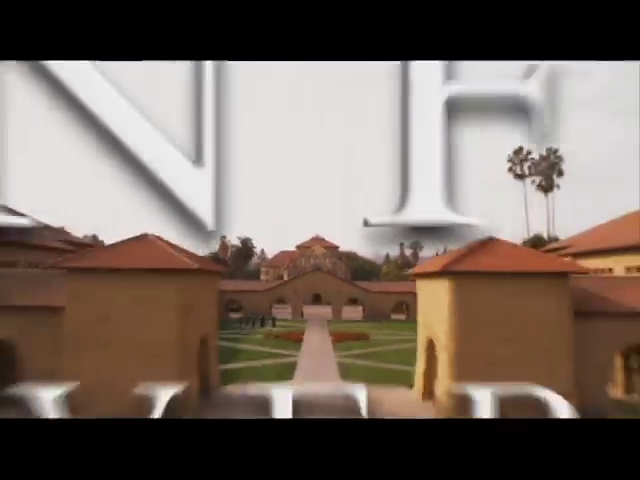
\includegraphics[width=0.78\textwidth]{lecture_02_figure_01.png}
  \caption{為後續連續極限預先整理的有限差分與黎曼和規則。}
  \lectureframe{00:04:20}
  \label{fig:l02-calculus-board}
\end{figure}

這些都是微積分中熟悉的定義。它們在此處的重要性在於標度：\(\Delta x_i\) 帶有一個 \(\Delta\sigma\) 的因子，而總和轉為積分時則帶有一個倒數因子。

\subsection{狄利克雷與諾伊曼端點條件}

有限區間上的傅立葉分析，從選擇端點條件開始。有兩種條件會反覆出現。

\begin{align}
  \text{Dirichlet:}\qquad
  &x(0)=x(\pi)=0,
  \label{eq:l02-dirichlet}\\
  \text{Neumann:}\qquad
  &\left.\partial_\sigma x\right|_{\sigma=0}
   =
   \left.\partial_\sigma x\right|_{\sigma=\pi}
   =0.
  \label{eq:l02-neumann}
\end{align}

兩端固定的提琴弦呈現狄利克雷條件：弦的位移在邊界處為零。諾伊曼函數在邊界處則不必為零；它在每個邊界處的斜率為零。黑板上並列呈現了這兩種典型形狀。

\begin{figure}[H]
  \centering
  \begin{minipage}[t]{0.48\textwidth}
    \centering
    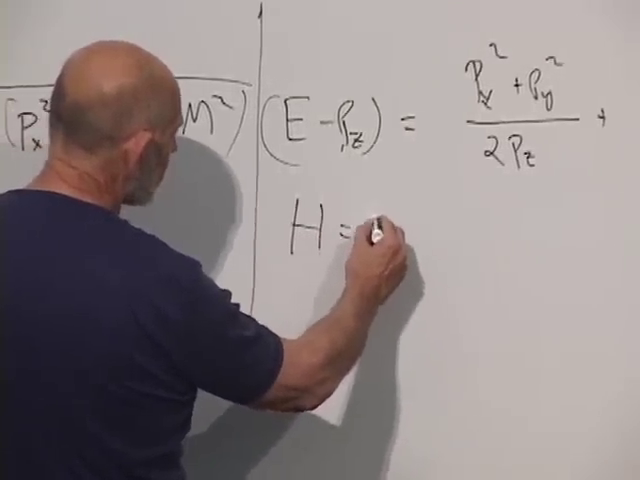
\includegraphics[width=\textwidth]{lecture_02_figure_02.png}
    \par\smallskip\footnotesize (a) 端點固定且斜率為零的形狀。
  \end{minipage}\hfill
  \begin{minipage}[t]{0.48\textwidth}
    \centering
    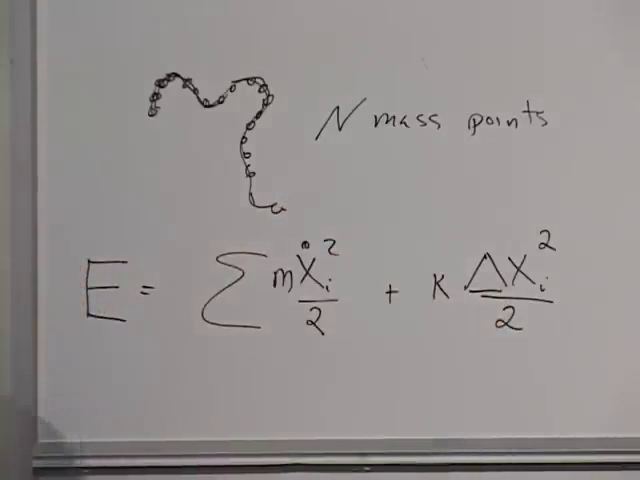
\includegraphics[width=\textwidth]{lecture_02_figure_03.png}
    \par\smallskip\footnotesize (b) 在豎直桿上滑動的輕環。
  \end{minipage}
  \caption{以形狀與力學呈現邊界條件。滑環模型明確描述了自由端點的橫向運動。}
  \lectureframe{00:08:50 and 00:12:15}
  \label{fig:l02-boundaries-board}
\end{figure}

\begin{figure}[H]
  \centering
  \begin{adjustbox}{max width=\linewidth}
  \begin{tikzpicture}[>=Latex,thick,scale=0.92]
    \begin{scope}
      \draw[->] (0,0) -- (4.4,0) node[right] {\(\sigma\)};
      \draw[->] (0,-1.25) -- (0,1.35) node[above] {\(x\)};
      \draw[blue!70!black]
        (0,0) .. controls (0.8,1.1) and (1.4,1.0) .. (2.0,0)
        .. controls (2.7,-1.0) and (3.4,-0.8) .. (4.1,0);
      \fill (0,0) circle (0.06);
      \fill (4.1,0) circle (0.06);
      \node at (2.05,-1.65) {Dirichlet: \(x=0\)};
    \end{scope}
    \begin{scope}[xshift=5.8cm]
      \draw[->] (0,0) -- (4.4,0) node[right] {\(\sigma\)};
      \draw[->] (0,-1.25) -- (0,1.35) node[above] {\(x\)};
      \draw[orange!85!black]
        (0,0.65) .. controls (0.8,0.65) and (1.1,-0.9) .. (2.0,-0.9)
        .. controls (2.9,-0.9) and (3.2,0.55) .. (4.1,0.55);
      \draw[orange!85!black] (0,0.65) -- (0.45,0.65);
      \draw[orange!85!black] (3.65,0.55) -- (4.1,0.55);
      \node at (2.05,-1.65) {Neumann: \(\partial_\sigma x=0\)};
    \end{scope}
  \end{tikzpicture}
  \end{adjustbox}
  \caption{狄利克雷條件固定函數值；諾伊曼條件固定斜率。}
  \label{fig:l02-boundaries-redraw}
\end{figure}

\begin{classroomqa}
\audiencequestion{開管或閉管風琴能否作為其中一種邊界條件的明確例子？\lecturetimestamp{00:09:19}}
\lecturerresponse{可以，但首先必須說明要展開的是哪個聲學變數。在理想化情況下，開口端的壓力擾動與縱向位移滿足互補的條件。與其在黑板上處理這個旁枝問題，不如採用滑環模型：近乎無質量的環能沿桿上下滑動，因此弦的端點是自由的，諾伊曼條件也一目了然。}
\end{classroomqa}

\begin{classroomqa}
\audiencequestion{圖形能否垂直上升，並包含尖銳的跳躍？\lecturetimestamp{00:09:53}}
\lecturerresponse{傅立葉分析容許分段連續函數有孤立跳躍，但物理弦受到更嚴格的限制。跳躍會使相鄰點斷開，並使空間導數 \(\partial_\sigma x\) 在下文推導的連續能量中變得奇異。因此，我們只考慮連續且可微的形狀。}
\end{classroomqa}

\begin{classroomqa}
\audiencequestion{為什麼管子的開口端，或任何自由端，都必須滿足邊界條件？\lecturetimestamp{00:11:14}}
\lecturerresponse{聲學例子取決於所選的場變數，講解中沒有進一步處理。力學例子則不同。極輕的環可以自由滑動，但仍與弦的最後一段相連。我們不預設端點條件，而是從牛頓定律推導：要使端點加速度有限，斜率就必須為零。}
\end{classroomqa}

\subsection{傅立葉基底}

端點條件的類別一旦確定，相應的傅立葉基底也就確定。在 \(0\leq\sigma\leq\pi\) 上，

\begin{align}
  x_D(\sigma)
  &=
  \sum_{n=1}^{\infty}x_n\sin(n\sigma),
  \label{eq:l02-dirichlet-series}\\
  x_N(\sigma)
  &=
  \sum_{n=0}^{\infty}x_n\cos(n\sigma).
  \label{eq:l02-neumann-series}
\end{align}

\eqref{eq:l02-dirichlet-series} 中的每個正弦函數在兩個端點都為零。
\eqref{eq:l02-neumann-series} 中的每個餘弦函數在端點處的導數都為零。
求和下限不同是有原因的：
\(\sin(0\sigma)=0\) 不會有貢獻，而
\(\cos(0\sigma)=1\) 是常數模態，也就是零模態。它代表諾伊曼函數的平均值。

\begin{figure}[H]
  \centering
  \begin{minipage}[t]{0.48\textwidth}
    \centering
    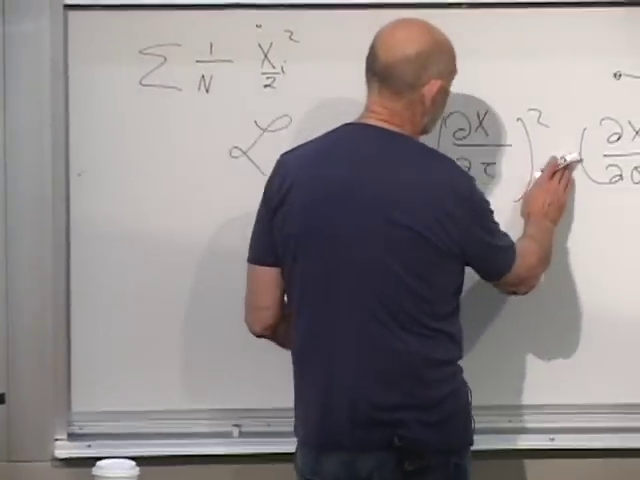
\includegraphics[width=\textwidth]{lecture_02_figure_04.png}
    \par\smallskip\footnotesize (a) 正弦與餘弦展開。
  \end{minipage}\hfill
  \begin{minipage}[t]{0.48\textwidth}
    \centering
    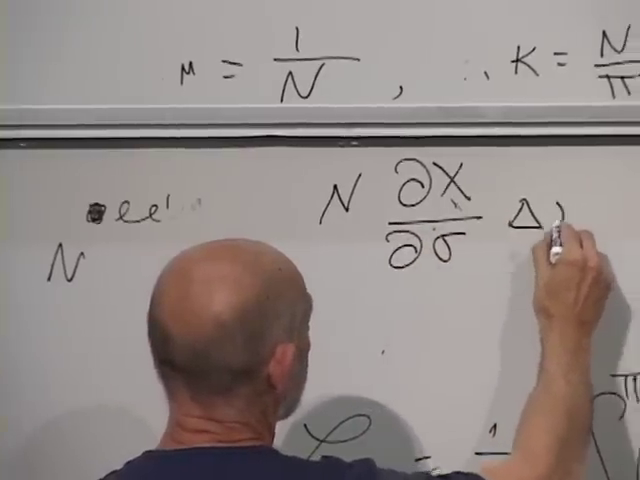
\includegraphics[width=\textwidth]{lecture_02_figure_05.png}
    \par\smallskip\footnotesize (b) 正交性與例外的
    常數模態。
  \end{minipage}
  \caption{後續將用來對角化弦的傅立葉性質。}
  \lectureframe{00:16:15 and 00:20:30}
  \label{fig:l02-fourier-board}
\end{figure}

微分會使這兩類互相轉換：

\begin{equation}
  \begin{aligned}
    \partial_\sigma\sin(n\sigma)&=n\cos(n\sigma),\\
    \partial_\sigma\cos(n\sigma)&=-n\sin(n\sigma).
  \end{aligned}
  \label{eq:l02-basis-derivatives}
\end{equation}

因此，狄利克雷級數的導數具有諾伊曼型態，而諾伊曼級數的導數則具有狄利克雷型態。接著，正交性會消去不同模態間的交叉項：

\begin{align}
  \int_0^\pi\cos(n\sigma)\cos(m\sigma)\,d\sigma
  &=
  \frac{\pi}{2}\delta_{nm},
  && n,m\geq1,
  \label{eq:l02-cos-orthogonality}\\
  \int_0^\pi\sin(n\sigma)\sin(m\sigma)\,d\sigma
  &=
  \frac{\pi}{2}\delta_{nm},
  && n,m\geq1,
  \label{eq:l02-sin-orthogonality}\\
  \int_0^\pi 1\,d\sigma&=\pi .
  \label{eq:l02-zero-norm}
\end{align}

最後一行是例外的 \(n=m=0\) 餘弦範數。常數模態的歸一化方式不同於非零諧波；這個二倍因子將區分弦的質心模態與內部模態。

\subsection{要記住的一個振子公式}

將座標重新標度，使其力學質量為一後，遵循虎克定律的振子具有

\begin{align}
  E_{\mathrm{osc}}
  &=
  \frac12\dot q^{\,2}
  +\frac12\omega^2q^2,
  \label{eq:l02-oscillator-energy}\\
  L_{\mathrm{osc}}
  &=
  \frac12\dot q^{\,2}
  -\frac12\omega^2q^2.
  \label{eq:l02-oscillator-lagrangian}
\end{align}

\begin{figure}[H]
  \centering
  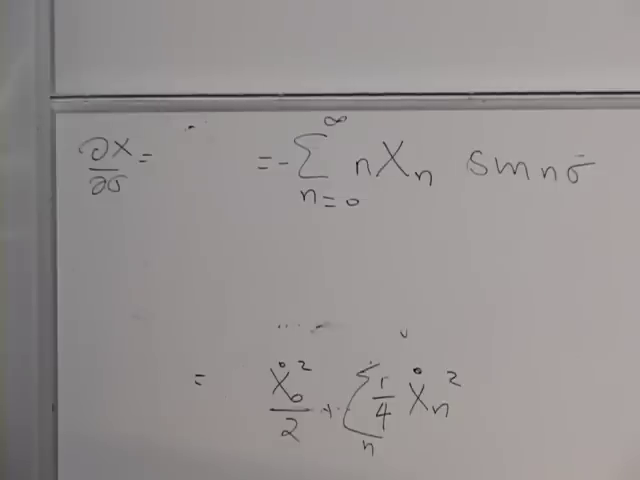
\includegraphics[width=0.68\textwidth]{lecture_02_figure_06.png}
  \caption{振子的能量寫成這個形式後，\(q^2\) 的係數便能
  直接看出 \(\omega^2\)。}
  \lectureframe{00:24:00}
  \label{fig:l02-oscillator-board}
\end{figure}

在經典力學中，\(\omega=\sqrt{\kappa/m}\)；座標重新標度後，\(m=1\)。在量子力學中，

\begin{equation}
  E_Q=\hbar\omega\left(Q+\frac12\right),
  \qquad Q=0,1,2,\ldots .
  \label{eq:l02-oscillator-spectrum}
\end{equation}

討論能級間距時，可以扣除各能級共有的基態能量，並說每個量子所需的能量為 \(\hbar\omega\)。弦的計算一開始也會這麼做，總零點能則留待之後處理。

\begin{classroomqa}
\audiencequestion{如何從能量公式看出振子的頻率？\lecturetimestamp{00:23:21}}
\lecturerresponse{重新標度之前，頻率為
\(\omega=\sqrt{\kappa/m}\)。質量設為一時，勢能項為
\(\frac12\omega^2q^2\)，因此它的二次項係數就是頻率的平方。}
\end{classroomqa}

\section{複合系統在什麼意義上算是粒子？}

弦具有延展性，我們會以許多彼此耦合的部分來建模。那麼，它的一個量子態在什麼意義上仍可稱為粒子？點狀性不能作為決定性判據。質子與中子都是複合粒子。電子與光子也受到量子場的修飾，儘管尚未測得其內在子結構。周圍空無一物的經典幾何點，並不是量子激發的恰當圖像。

光有質量與質心位置也不足以構成判據。密封的氣體箱兩者兼具，一杯咖啡也一樣；我們通常不會把它們稱為粒子。不可分性同樣不是判據，因為質子可以分解；自旋也無法區分微觀粒子與宏觀物體。

有用的判據是能譜是否隔離。將靜止能量標在縱軸上，再問要增加多少能量才能到達另一個內部態。電子附近沒有實驗可及的電子激發態序列。質子則有共振態，但最低幾個共振態所需能量達數百 MeV，約為質子質量的相當一部分。這些態彼此分隔得夠遠，因此能逐一辨識。

一杯咖啡的情形正好相反。只要加入任意微小的能量，就能激發長波長聲模態、推動分子，或產生聲子。極大量的態密集分布在極小的能量區間內；在實驗室尺度上，它們構成連續譜。這就是粒子與\emph{一團混沌}之間實際上的差別。

\begin{figure}[H]
  \centering
  \includegraphics[width=0.58\textwidth]{lecture_02_figure_07.png}
  \caption{比較孤立的粒子能級與普通物質密集的激發態時，黑板上的縱向能量軸。}
  \lectureframe{00:31:10}
  \label{fig:l02-spectrum-board}
\end{figure}

\begin{figure}[H]
  \centering
  \begin{adjustbox}{max width=\linewidth}
  \begin{tikzpicture}[>=Latex,thick]
    \begin{scope}
      \draw[->] (0,0) -- (0,4.8) node[above] {energy};
      \draw[blue!70!black,line width=1.2pt] (-1.0,0.65) -- (1.0,0.65);
      \draw[blue!70!black,line width=1.2pt] (-1.0,3.65) -- (1.0,3.65);
      \node[right] at (1.05,0.65) {ground state};
      \node[right] at (1.05,3.65) {first internal excitation};
      \draw[<->] (0.65,0.75) -- (0.65,3.55)
        node[midway,right] {large gap};
      \node at (0,-0.55) {particle-like};
    \end{scope}
    \begin{scope}[xshift=7.0cm]
      \draw[->] (0,0) -- (0,4.8) node[above] {energy};
      \foreach \y in {0.55,0.69,0.82,0.94,1.05,1.15,1.24,1.32,1.39,1.45,
        1.51,1.57,1.63,1.70,1.78,1.87,1.97,2.09,2.22,2.36,2.51,2.67,2.84,
        3.02,3.21,3.41,3.62,3.84,4.07}
        \draw[orange!85!black] (-0.95,\y) -- (0.95,\y);
      \node[right] at (1.05,2.25) {dense phonon and internal states};
      \node at (0,-0.55) {macroscopic matter};
    \end{scope}
  \end{tikzpicture}
  \end{adjustbox}
  \caption{講座採用的操作性粒子判據是能譜隔離，而非字面上的點狀性。}
  \label{fig:l02-particle-redraw}
\end{figure}

這項判據將哲學問題轉化為計算：量子化弦，找出它的內部能級，再檢視能級間距。如果弦的第一激發態位於普朗克尺度附近，而觀測到的基態質量很小，那麼兩者間的能隙就比目前加速器所能達到的能量高出二十多個數量級。在所有可及的能量範圍內，弦因此都會呈現基本粒子的行為。

\begin{classroomqa}
\audiencequestion{粒子行為只是觀測尺度的問題嗎？如果放大到足夠大的程度，能級會不再彼此分離嗎？\lecturetimestamp{00:33:33}}
\lecturerresponse{放大可能揭露物體由許多組分構成，但不會消除它的能譜。關鍵在於比較實驗的能量解析度與第一個內部激發態的能隙。只要能隙極大，複合物體仍可能呈現粒子般的行為。}
\end{classroomqa}

\begin{classroomqa}
\audiencequestion{為什麼普通的小提琴弦不是粒子？\lecturetimestamp{00:34:37}}
\lecturerresponse{一個振動量子所帶的能量，與宏觀弦的靜止能量相比小得無法測量。因此，在極小的相對能量區間內就有許多量子態。它屬於能譜比較中密集的一側，而非孤立的一側。}
\end{classroomqa}

\begin{classroomqa}
\audiencequestion{如果量子場以虛擬漲落修飾光子與電子，它們還算是點粒子嗎？\lecturetimestamp{00:35:40}}
\lecturerresponse{經典意義下的\emph{點}這個詞承載了太多含義。實際的電子與光子是受到場修飾的激發態，但實驗尚未發現它們具有內在組分結構或有限的形狀因子。就目前的論證而言，重點是兩者都沒有密集、近乎簡併的內部態序列。\editorialnote{講座將電子的反常磁矩與可測量的量子模糊性聯繫起來。以現代術語來說，反常磁矩是輻射修飾效應，並非電子具有可分辨有限半徑的證據。依照慣例，所謂點狀，是指在已測試的尺度內尚未探測到內在子結構或形狀因子。}}
\end{classroomqa}

\begin{classroomqa}
\audiencequestion{光子的大小會隨頻率改變嗎？\lecturetimestamp{00:36:49}}
\lecturerresponse{光子的波長確實取決於頻率，但那與內在的組分大小不同。改變頻率會改變波包與波長，不會改變光子可分辨的內部半徑。}
\end{classroomqa}

\section{大動量下的精確橫向力學}

現在回到相對論帶來的困難。不能只把快速旋轉的短棒質心置於靜止，就將它視為非相對論系統；短棒兩端彼此之間仍作相對論性運動。非相對論近似失效的原因，是系統內部存在相對運動。

然而，還有另一種極限。選定 \(z\) 軸，並對整個系統沿該軸作洛倫茲 boost，使縱向動量 \(P_z\) 變得極大。保持其橫向動量

\begin{equation}
  p_\perp^2=p_x^2+p_y^2
\end{equation}

有限。在 \(P_z\to\infty\) 的極限下，橫向投影可精確寫成非相對論哈密頓量的形式，即使 boost 前的內部運動原本具有相對論性。

\begin{classroomqa}
\audiencequestion{無限動量是否代表有質量的系統實際上達到了光速？\lecturetimestamp{00:40:43}}
\lecturerresponse{任何有限的 boost 都無法使它達到光速。我們所構造的是在 \(P_z\) 任意增大時具有良好定義極限的物理量。這個說法指的是一種取極限的程序，而不是具有 \(v=c\) 的有限物理狀態。}
\end{classroomqa}

\begin{classroomqa}
\audiencequestion{應該選哪個軸？如果物體繞著該軸旋轉，或在垂直於該軸的方向上運動，又會如何？\lecturetimestamp{00:41:14}}
\lecturerresponse{可以選擇任意軸，並沿該軸對整個系統作 boost。明確保留下來的力學，是物體在垂直平面上的投影。一根旋轉的桿可能看起來縮短了，也可能掃過該平面，但它的橫向投影仍具有非相對論形式。}
\end{classroomqa}

弦還有一項性質，使這種描述格外有力。在光前規範中，弦的縱向內部座標不是獨立的振子，而是由約束根據橫向運動決定。因此，只要知道弦的橫向狀態，就足以重建其物理自由度。

\begin{classroomqa}
\audiencequestion{沒有獨立的縱向座標，是否代表弦只是被困在一個薄薄的夾層中？\lecturetimestamp{00:42:26}}
\lecturerresponse{洛倫茲收縮確實會使弦在 boost 後參考系中的縱向延展變小，但這裡的論述更強。任何剩餘的縱向運動都受橫向運動約束，不能獨立指定。}
\end{classroomqa}

\begin{classroomqa}
\audiencequestion{這種將描述化約為橫向資料的做法，與全息原理有關嗎？\lecturetimestamp{00:43:12}}
\lecturerresponse{它與促成全息思想的思路密切相關，不過探討這項關聯會使我們偏離目前的計算。在此處，這項關聯只用來說明為何可以只處理弦的橫向部分。}
\end{classroomqa}

\subsection{扣除 boost 能量並重新標度時間}

設 \(M\) 為整個系統的不變質量，包含組分質量、動能與束縛能。在 \(c=1\) 單位制下，

\begin{equation}
  E=\sqrt{P_z^2+p_\perp^2+M^2}.
  \label{eq:l02-relativistic-energy}
\end{equation}

當 \(P_z\) 遠大於 \(p_\perp\) 與 \(M\) 時，

\begin{equation}
  E
  =
  P_z+\frac{p_\perp^2+M^2}{2P_z}
  +O(P_z^{-3}).
  \label{eq:l02-large-pz}
\end{equation}

\begin{figure}[H]
  \centering
  \includegraphics[width=0.76\textwidth]{lecture_02_figure_08.png}
  \caption{完整的高 \(P_z\) 展開式，保留了橫向動量與不變質量。}
  \lectureframe{00:47:30}
  \label{fig:l02-large-pz-board}
\end{figure}

領先項很大，卻不含任何內部狀態的資訊。若過程中 \(P_z\) 守恆，例如受 boost 的原子在總縱向動量不變時於內部能級間躍遷，這一項就會從所有能量差中抵消。因此我們研究

\begin{equation}
  E-P_z=\frac{p_\perp^2+M^2}{2P_z}+O(P_z^{-3}).
  \label{eq:l02-residual-energy}
\end{equation}

分母具有物理意義。哈密頓量生成時間演化，因此微小的剩餘能量表示內部演化在實驗室時間中看來較慢，這就是時間膨脹。若要保留內部運動，可引入重新標度後的演化參數 \(\tau\)，或等價地將剩餘哈密頓量乘以 \(P_z\)：

\begin{equation}
  H_\perp
  \equiv
  \lim_{P_z\to\infty}P_z(E-P_z)
  =
  \frac12p_\perp^2+\frac12M^2.
  \label{eq:l02-transverse-hamiltonian}
\end{equation}

\begin{figure}[H]
  \centering
  \begin{minipage}[t]{0.48\textwidth}
    \centering
    \includegraphics[width=\textwidth]{lecture_02_figure_09.png}
    \par\smallskip\footnotesize (a) \(H=i\partial_t\) 與變慢的內部
    演化。
  \end{minipage}\hfill
  \begin{minipage}[t]{0.48\textwidth}
    \centering
    \includegraphics[width=\textwidth]{lecture_02_figure_10.png}
    \par\smallskip\footnotesize (b) 重新標度時間後的有限橫向哈密頓量。
  \end{minipage}
  \caption{從因時間膨脹而變小的剩餘能量，得到有限的
  二維哈密頓量。}
  \lectureframe{00:49:20 and 00:52:40}
  \label{fig:l02-lightfront-board}
\end{figure}

這正是單位質量粒子在二維中運動的形式：動能 \(p_\perp^2/2\) 加上內部能量 \(M^2/2\)。特別之處在於平方項。在這種描述中，扮演靜止能量或束縛能角色的量，正比於不變質量的平方。\editorialnote{採用傳統的光前變數 \(P^\pm=(E\pm P_z)/\sqrt2\) 時，精確的質殼關係為 \(2P^+P^-=p_\perp^2+M^2\)。方程 \eqref{eq:l02-transverse-hamiltonian} 則是本講以高 \(P_z\) 為基準正規化後的同一不變關係。}

\begin{classroomqa}
\audiencequestion{複合系統中各個組成部分的縱向動量去哪裡了？\lecturetimestamp{00:51:30}}
\lecturerresponse{一般的複合物體必須保留各組分所帶總 \(P_z\) 的比例。上面的公式使用的是總質心動量。弦論的特殊之處，在於其約束可由橫向自由度決定相對縱向運動，因此不必另外加入獨立的縱向振子。}
\end{classroomqa}

\section{離散開弦}

現在，弦明確地只在橫向平面中運動。將兩個座標標記為 \(X\) 與 \(Y\)，並先以 \(N\) 個質點和連接它們的 \(N-1\) 根彈簧近似弦。若 \(\mu\) 是每個質點的類比質量，而 \(k\) 是最近鄰彈簧常數，則能量為

\begin{equation}
  E_N
  =
  \sum_i
  \left[
    \frac{\mu}{2}
    \left(\dot X_i^2+\dot Y_i^2\right)
    +
    \frac{k}{2}
    \left((\Delta X_i)^2+(\Delta Y_i)^2\right)
  \right].
  \label{eq:l02-discrete-energy}
\end{equation}

每個 \(X\) 項都有一個相同的 \(Y\) 項，因為橫向平面有兩個方向。指標 \(i\) 標示鏈上的點，並非空間座標。

\begin{figure}[H]
  \centering
  \begin{minipage}[t]{0.48\textwidth}
    \centering
    \includegraphics[width=\textwidth]{lecture_02_figure_11.png}
    \par\smallskip\footnotesize (a) 質點鏈及其離散能量。
  \end{minipage}\hfill
  \begin{minipage}[t]{0.48\textwidth}
    \centering
    \includegraphics[width=\textwidth]{lecture_02_figure_12.png}
    \par\smallskip\footnotesize (b) \(N\) 增大時 \(\mu\) 與 \(k\) 的標度變化。
  \end{minipage}
  \caption{取連續極限前的正則化開弦。}
  \lectureframe{00:57:42 and 01:02:40}
  \label{fig:l02-chain-board}
\end{figure}

\begin{figure}[H]
  \centering
  \begin{adjustbox}{max width=\linewidth}
  \begin{tikzpicture}[>=Latex,thick]
    \foreach \i in {0,...,8} {
      \coordinate (p\i) at ({1.05*\i},{0.30*sin(55*\i)});
      \filldraw[white] (p\i) circle (0.10);
      \draw (p\i) circle (0.10);
    }
    \foreach \i in {0,...,7} {
      \pgfmathtruncatemacro{\j}{\i+1}
      \draw[decorate,decoration={zigzag,segment length=4pt,amplitude=2pt}]
        (p\i) -- (p\j);
    }
    \node[above=0.35cm of p0] {\(i=0\)};
    \node[above=0.35cm of p8] {\(i=N-1\)};
    \draw[<->] (0,-1.15) -- (8.4,-1.15)
      node[midway,below] {\(0\leq\sigma\leq\pi\)};
    \node at (4.2,1.25)
      {\(\mu=1/N,\quad k=N/\pi^2,\quad\Delta\sigma=\pi/N\)};
  \end{tikzpicture}
  \end{adjustbox}
  \caption{清楚的正則化示意圖。鏈逐漸細分時，質點會變輕，而微觀彈簧會變硬。}
  \label{fig:l02-chain-redraw}
\end{figure}

參數 \(\sigma\) 標示沿鏈的位置。選擇 \(0\leq\sigma\leq\pi\) 是一種約定，並非對物理長度的測量。這提醒我們弦有兩個端點。稍後，閉弦的位置將以 \(0\leq\sigma<2\pi\) 為週期標記。

連續極限必須使整體力學量保持有限。若每個質點的質量固定，總類比質量就會發散，因此取

\begin{equation}
  \mu=\frac{1}{N}.
  \label{eq:l02-mu-scaling}
\end{equation}

於是 \(N\mu=1\)。這不是相對論中的靜止質量 \(M\)，而是橫向類比模型中的慣性係數。

串聯彈簧的數目增加時，整體會變軟。若要使整條鏈的勁度保持有限，每根微觀彈簧就必須變硬：

\begin{equation}
  k=\frac{N}{\pi^2}
  =\frac{1}{\pi\,\Delta\sigma}.
  \label{eq:l02-k-scaling}
\end{equation}

只有 \(k\propto N\) 是必要的。因子 \(\pi^2\) 是一種正規化選擇，用來從連續公式中消除多餘的 \(\pi\) 因子。

\begin{classroomqa}
\audiencequestion{\(\mu\) 是每個弦點的物理靜止質量嗎？\lecturetimestamp{01:10:34}}
\lecturerresponse{不是。它是橫向質點鏈中的非相對論類比質量。稱它為 \(M\)，會使人將它與整個相對論弦態的不變靜止質量混淆。它在此處的唯一用途，是產生正確的連續極限慣性。}
\end{classroomqa}

\section{連續波動系統}

套用開頭整理好的規則。由於
\(1/N=\Delta\sigma/\pi\)，

\begin{align}
  \sum_i\frac{\mu}{2}\dot X_i^2
  &=
  \frac{1}{2\pi}
  \sum_i\dot X_i^2\,\Delta\sigma
  \longrightarrow
  \frac{1}{2\pi}
  \int_0^\pi
  \left(\partial_\tau X\right)^2d\sigma ,
  \label{eq:l02-kinetic-limit}\\
  \sum_i\frac{k}{2}(\Delta X_i)^2
  &\longrightarrow
  \frac{1}{2\pi}
  \int_0^\pi
  \left(\partial_\sigma X\right)^2d\sigma .
  \label{eq:l02-potential-limit}
\end{align}

第二行使用
\(\Delta X_i=\partial_\sigma X\,\Delta\sigma\) 以及
\(k=1/(\pi\Delta\sigma)\)。對 \(Y\) 也可作相同計算。

\begin{figure}[H]
  \centering
  \begin{minipage}[t]{0.48\textwidth}
    \centering
    \includegraphics[width=\textwidth]{lecture_02_figure_13.png}
    \par\smallskip\footnotesize (a) 將總和轉為積分，並將
    差分轉為導數。
  \end{minipage}\hfill
  \begin{minipage}[t]{0.48\textwidth}
    \centering
    \includegraphics[width=\textwidth]{lecture_02_figure_14.png}
    \par\smallskip\footnotesize (b) 完成連續極限後的能量。
  \end{minipage}
  \caption{離散鏈在 \(\sigma\) 區間上轉變為場。}
  \lectureframe{01:05:40 and 01:07:00}
  \label{fig:l02-continuum-board}
\end{figure}

因此得到的能量與拉格朗日量為

\begin{align}
  E
  &=
  \frac{1}{2\pi}
  \int_0^\pi d\sigma\,
  \left[
    (\partial_\tau X)^2+(\partial_\tau Y)^2\right.\notag\\[-0.25em]
  &\hspace{6.5em}\left.
    +(\partial_\sigma X)^2+(\partial_\sigma Y)^2
  \right],
  \label{eq:l02-continuum-energy}\\
  L
  &=
  \frac{1}{2\pi}
  \int_0^\pi d\sigma\,
  \left[
    (\partial_\tau X)^2+(\partial_\tau Y)^2\right.\notag\\[-0.25em]
  &\hspace{6.5em}\left.
    -(\partial_\sigma X)^2-(\partial_\sigma Y)^2
  \right].
  \label{eq:l02-continuum-lagrangian}
\end{align}

\begin{figure}[H]
  \centering
  \includegraphics[width=0.78\textwidth]{lecture_02_figure_15.png}
  \caption{連續極限下的拉格朗日量，其中動能項與拉伸項
  的符號相反。}
  \lectureframe{01:08:48}
  \label{fig:l02-lagrangian-board}
\end{figure}

若將 \(\sigma\) 改稱為一般的空間座標，並將 \(X\) 改稱為場 \(\phi\)，這些就是一維波場的能量與拉格朗日量。對 \eqref{eq:l02-continuum-lagrangian} 作變分，得到

\begin{equation}
  \left(\partial_\tau^2-\partial_\sigma^2\right)X=0,
  \qquad
  \left(\partial_\tau^2-\partial_\sigma^2\right)Y=0.
  \label{eq:l02-wave-equation}
\end{equation}

眼前的論證不需要直接求解這些方程。只要掌握以下圖像即可：波沿弦向左、向右傳播，並在端點反射。狄利克雷反射會使位移反號；諾伊曼反射則保持位移的符號。

\begin{classroomqa}
\audiencequestion{時間變數 \(\tau\) 究竟是什麼？\lecturetimestamp{01:08:54}}
\lecturerresponse{它是在高 \(P_z\) 描述中追蹤內部運動的重新標度時間。與系統一同受 boost 的時鐘相較於實驗室時鐘走得較慢；\(\tau\) 可消除這種時間膨脹，使內部振盪維持有限的頻率。對這裡討論的橫向力學而言，可以直接把它當作時間。\editorialnote{講義非正式地將 \(\tau\) 稱為固有時。對延展的弦而言，精確的光前演化參數是經過規範固定的重新標度時間，而不是所有弦上位置共用的單一不變固有時。這不影響原本的時間膨脹論證。}}
\end{classroomqa}

當質心在橫向平面中靜止時，\eqref{eq:l02-continuum-energy} 的內部部分，依照 \eqref{eq:l02-transverse-hamiltonian} 的正規化，正比於 \(M^2\)。因此，量子化這個表面上尋常的波動系統，就能揭示相對論性的質量譜。

\begin{classroomqa}
\audiencequestion{\(P_z(E-P_z)\) 有名稱嗎？\lecturetimestamp{01:11:00}}
\lecturerresponse{它通常稱為光錐能量或光前能量。「光前」更能描述作為演化曲面的零平面；採用哪個傳統術語，並不影響計算。}
\end{classroomqa}

\begin{classroomqa}
\audiencequestion{「錐」是指一般時空中的光錐嗎？這個術語是 Dirac 提出的嗎？\lecturetimestamp{01:11:17}}
\lecturerresponse{零座標的構造可以用 45 度軸繪出，但此處的演化曲面是光前，而非完整的膨脹光錐。Dirac 曾發展相關的相對論動力學形式；至於名稱的歷史由來，講解中並未定論，也不影響方程。}
\end{classroomqa}

\section{為什麼自由端點滿足諾伊曼條件}

現在可以推導端點條件，而不必預先假設。由於經過 boost 的橫向力學恰好具有非相對論形式，因此可以使用牛頓定律。內部質點受到兩側彈簧的拉力；末端質點則只受到連接相鄰質點的那根彈簧拉力。

\begin{classroomqa}
\audiencequestion{討論相對論性弦時，為什麼可以使用牛頓定律？\lecturetimestamp{01:14:52}}
\lecturerresponse{我們並非將牛頓力學用於未經 boost 的完整時空運動，而是用於無限動量描述中的橫向變數；這些變數的哈密頓量恰好具有非相對論形式。}
\end{classroomqa}

在右端點，依虎克定律，力為（正負號取決於方向）

\begin{equation}
  F_{\mathrm{end}}
  =
  -k\,\Delta X
  =
  -\frac{1}{\pi\Delta\sigma}
   \left(\partial_\sigma X\,\Delta\sigma\right)
  =
  -\frac{1}{\pi}\partial_\sigma X .
  \label{eq:l02-endpoint-force}
\end{equation}

\begin{figure}[H]
  \centering
  \begin{minipage}[t]{0.48\textwidth}
    \centering
    \includegraphics[width=\textwidth]{lecture_02_figure_16.png}
    \par\smallskip\footnotesize (a) 端點受力與當地
    斜率成正比。
  \end{minipage}\hfill
  \begin{minipage}[t]{0.48\textwidth}
    \centering
    \includegraphics[width=\textwidth]{lecture_02_figure_17.png}
    \par\smallskip\footnotesize (b) 有限加速度條件。
  \end{minipage}
  \caption{以牛頓定律推導自由端的邊界條件。}
  \lectureframe{01:18:20 and 01:20:10}
  \label{fig:l02-neumann-board}
\end{figure}

末端質點的牛頓運動方程為

\begin{equation}
  \mu\,\partial_\tau^2X=F_{\mathrm{end}},
  \qquad
  \mu=\frac1N=\frac{\Delta\sigma}{\pi}.
  \label{eq:l02-endpoint-newton}
\end{equation}

合併 \eqref{eq:l02-endpoint-force} 與
\eqref{eq:l02-endpoint-newton}，

\begin{equation}
  \partial_\sigma X
  =
  -\Delta\sigma\,\partial_\tau^2X
  \quad\text{at the right endpoint},
  \label{eq:l02-endpoint-scaling}
\end{equation}

左端點的受力方向相反。若 \(\partial_\sigma X\) 在
\(\Delta\sigma\to0\) 時趨近非零常數，端點加速度就會如 \(N\) 般發散。
因此，要使連續極限合理且加速度有限，就必須有

\begin{equation}
  \left.\partial_\sigma X\right|_{0,\pi}=0,
  \qquad
  \left.\partial_\sigma Y\right|_{0,\pi}=0.
  \label{eq:l02-open-neumann}
\end{equation}

\begin{figure}[H]
  \centering
  \begin{adjustbox}{max width=\linewidth}
  \begin{tikzpicture}[>=Latex,thick,scale=1.0]
    \coordinate (a) at (0,0);
    \coordinate (b) at (4.5,0.75);
    \filldraw[white] (a) circle (0.12);
    \draw (a) circle (0.12);
    \filldraw[white] (b) circle (0.12);
    \draw (b) circle (0.12);
    \draw[decorate,decoration={zigzag,segment length=6pt,amplitude=3pt}]
      (a) -- (b);
    \draw[dashed] (a) -- (0,-1.2);
    \draw[dashed] (b) -- (4.5,-1.2);
    \draw[<->] (4.85,0) -- (4.85,0.75)
      node[midway,right] {\(\Delta X\)};
    \draw[->,red!70!black] (b) -- (5.75,0.95)
      node[right] {\(F_{\rm end}=-k\Delta X\)};
    \node[below] at (0,-1.2) {\(N-1\)};
    \node[below] at (4.5,-1.2) {\(N\)};
    \node at (2.5,-2.0)
      {\(\mu\ddot X=-k\Delta X
      \ \Longrightarrow\
      \partial_\sigma X=-\Delta\sigma\,\ddot X\to0\)};
  \end{tikzpicture}
  \end{adjustbox}
  \caption{在正則化極限下，末端質點的質量趨近於零。只有端點斜率趨近於零，
  加速度才可能有限。}
  \label{fig:l02-neumann-redraw}
\end{figure}

對兩端與兩個橫向方向作相同論證，就得到自由開弦的諾伊曼邊界條件。

\section{開弦的簡正模態}

現在我們已經得到完整的古典系統，包括拉格朗日量與邊界條件。經過傅立葉分析後，量子化就變得簡單。由於端點滿足諾伊曼條件，

\begin{align}
  X(\sigma,\tau)
  &=
  \sum_{n=0}^{\infty}X_n(\tau)\cos(n\sigma),
  \label{eq:l02-X-expansion}\\
  Y(\sigma,\tau)
  &=
  \sum_{n=0}^{\infty}Y_n(\tau)\cos(n\sigma).
  \label{eq:l02-Y-expansion}
\end{align}

所有 \(\sigma\) 依賴都包含在餘弦函數中；所有時間依賴則包含在係數中。\(X_n(\tau)\) 與 \(Y_n(\tau)\) 隨時間改變，弦也因此振動。

\begin{figure}[H]
  \centering
  \includegraphics[width=0.78\textwidth]{lecture_02_figure_18.png}
  \caption{尼曼模態展開式與將使雙重求和化簡的正交關係並列。}
  \lectureframe{01:21:45}
  \label{fig:l02-mode-expansion-board}
\end{figure}

\subsection{動能項與零模}

對時間微分可得

\begin{equation}
  \partial_\tau X
  =
  \sum_{n=0}^{\infty}\dot X_n(\tau)\cos(n\sigma).
  \label{eq:l02-time-mode}
\end{equation}

平方後會得到對 \(n\) 和 \(m\) 的雙重求和，但
\eqref{eq:l02-cos-orthogonality}會消去所有滿足 \(n\neq m\) 的項。
將常數模另行處理，

\begin{equation}
  \frac{1}{2\pi}\int_0^\pi
  (\partial_\tau X)^2\,d\sigma
  =
  \frac12\dot X_0^{\,2}
  +
  \frac14\sum_{n=1}^{\infty}\dot X_n^{\,2}.
  \label{eq:l02-mode-kinetic}
\end{equation}

\begin{figure}[H]
  \centering
  \includegraphics[width=0.76\textwidth]{lecture_02_figure_19.png}
  \caption{正交性積分將動能的雙重求和化為零模項與對角求和。}
  \lectureframe{01:29:10}
  \label{fig:l02-mode-kinetic-board}
\end{figure}

常數係數就是平均位置，

\begin{equation}
  X_0(\tau)=\frac1\pi\int_0^\pi X(\sigma,\tau)\,d\sigma ,
  \label{eq:l02-center-of-mass}
\end{equation}

對 \(Y_0\) 也一樣。在均勻的類比質量密度下，這些就是質心座標。它們具有動能，卻沒有恢復力：整條弦可以在橫向平面中自由移動。

\subsection{拉伸項與振子頻率}

對空間微分可得

\begin{equation}
  \partial_\sigma X
  =
  -\sum_{n=1}^{\infty}nX_n(\tau)\sin(n\sigma).
  \label{eq:l02-spatial-mode}
\end{equation}

零模消失了，因為均勻平移不會拉伸弦。利用正弦函數的正交性，

\begin{equation}
  \frac{1}{2\pi}\int_0^\pi
  (\partial_\sigma X)^2\,d\sigma
  =
  \frac14\sum_{n=1}^{\infty}n^2X_n^{\,2}.
  \label{eq:l02-mode-potential}
\end{equation}

\begin{figure}[H]
  \centering
  \includegraphics[width=0.76\textwidth]{lecture_02_figure_20.png}
  \caption{對餘弦級數微分後會得到正弦函數的雙重求和；正交性再次要求 \(n=m\)。}
  \lectureframe{01:31:40}
  \label{fig:l02-mode-potential-board}
\end{figure}

因此，\(X\) 部分的拉格朗日量為

\begin{equation}
  L_X
  =
  \frac12\dot X_0^{\,2}
  +
  \frac14\sum_{n=1}^{\infty}
  \left(
    \dot X_n^{\,2}-n^2X_n^{\,2}
  \right),
  \label{eq:l02-X-lagrangian}
\end{equation}

\(Y\) 也有相同的表示式。相應的能量中，\(n^2X_n^2\) 前的係數為正。每個非零模都是獨立的諧振子；與 \eqref{eq:l02-oscillator-lagrangian} 比較可得

\begin{equation}
  \omega_n=n,
  \qquad n=1,2,3,\ldots .
  \label{eq:l02-mode-frequency}
\end{equation}

\begin{figure}[H]
  \centering
  \includegraphics[width=0.80\textwidth]{lecture_02_figure_21.png}
  \caption{解耦振子的拉格朗日量，以及結論 \(\omega_n=n\)；下方也列出完全相同的 \(Y\) 模態序列。}
  \lectureframe{01:35:50}
  \label{fig:l02-oscillator-modes-board}
\end{figure}

簡正模就是弦的各個諧波。第一諧波緩慢地彎曲，第二諧波的頻率是第一諧波的兩倍，第三諧波則是三倍，依此類推。正交性使不同諧波在自由理論中彼此不耦合。

\begin{classroomqa}
\audiencequestion{\(n=0\)振子怎麼了？\lecturetimestamp{01:34:49}}
\lecturerresponse{它的頻率為零，因為它根本不是內部振子，而是讓質心平移的自由度。沒有彈簧會把整條弦恢復到某個偏好的橫向位置，因此零模是自由粒子的座標。}
\end{classroomqa}

扣除質心的動能項後，剩下的就是內部能量

\begin{equation}
  E_{\mathrm{int}}
  =
  \frac14
  \sum_{n=1}^{\infty}
  \left[
    \dot X_n^{\,2}+n^2X_n^{\,2}
    +\dot Y_n^{\,2}+n^2Y_n^{\,2}
  \right].
  \label{eq:l02-internal-energy}
\end{equation}

在光前座標的歸一化下，這與弦態的不變質量平方成正比。如此一來，我們便將相對論性的質量問題轉化為兩列可數振子模態的量子力學。

\section{量子化能階與粒子行為}

令 \(a_n^\dagger\) 在頻率為 \(n\) 的 \(X\) 振子中產生一個量子，\(b_n^\dagger\) 則在 \(Y\) 振子中做同樣的事。本講稍後才會系統性地討論算符，但這套記號能清楚呈現能階計數。相對於基態能量位移，

\begin{equation}
  \begin{aligned}
    \Delta E_{\mathrm{int}}
    &=\sum_{n=1}^{\infty}n\left(Q_n^X+Q_n^Y\right),\\
    Q_n^X,Q_n^Y&\in\{0,1,2,\ldots\}.
  \end{aligned}
  \label{eq:l02-quantized-energy}
\end{equation}

其中 \(\hbar=1\)。整數 \(n\) 標示受到激發的是哪個振子；\(Q_n\) 則計數該振子中佔據的量子數。\editorialnote{每個振子也會貢獻零點能。這個無窮和需要正則化，並決定弦質量公式中的截距。本講在此刻意不指定基態能量位移，只計算激發能階。}

振子真空 \(\ket{0}\) 並非空無一物的時空，而是一條內部振子都未受激發的開弦。它具有能量與動量，並在弦譜中有確定的位置。

第一能階有兩個態：

\begin{equation}
  a_1^\dagger\ket{0},
  \qquad
  b_1^\dagger\ket{0},
  \label{eq:l02-level-one}
\end{equation}

它們對應於沿 \(X\) 或 \(Y\) 極化的最低諧波。任意橫向極化都可由線性組合描述。

第二能階有五個態：

\begin{equation}
  (a_1^\dagger)^2\ket{0},
  \quad
  a_1^\dagger b_1^\dagger\ket{0},
  \quad
  (b_1^\dagger)^2\ket{0},
  \quad
  a_2^\dagger\ket{0},
  \quad
  b_2^\dagger\ket{0}.
  \label{eq:l02-level-two}
\end{equation}

其中三個由第一諧波的兩個量子構成，另外兩個則各由第二諧波的一個量子構成。這兩種組態的能量都增加兩個單位。

\begin{figure}[H]
  \centering
  \includegraphics[width=0.76\textwidth]{lecture_02_figure_22.png}
  \caption{聽眾提出質疑後，重新清點第二能階的五個態：兩個雙量子激發態、一個混合激發態，以及兩個第二諧波激發態。}
  \lectureframe{01:44:00}
  \label{fig:l02-levels-board}
\end{figure}

\begin{figure}[H]
  \centering
  \begin{adjustbox}{max width=\linewidth}
  \begin{tikzpicture}[>=Latex,thick]
    \draw[->] (0,0) -- (0,5.1) node[above] {\(\Delta E_{\rm int}\)};
    \draw[blue!70!black] (-0.65,0.55) -- (0.65,0.55);
    \node[right] at (0.85,0.55) {\(\ket{0}\) \quad multiplicity \(1\)};
    \draw[blue!70!black] (-0.65,2.15) -- (0.65,2.15);
    \node[right] at (0.85,2.15)
      {\(a_1^\dagger\ket{0},\ b_1^\dagger\ket{0}\)
      \quad multiplicity \(2\)};
    \draw[blue!70!black] (-0.65,3.75) -- (0.65,3.75);
    \node[right,text width=8.6cm] at (0.85,3.75)
      {\((a_1^\dagger)^2\ket{0},
      a_1^\dagger b_1^\dagger\ket{0},
      (b_1^\dagger)^2\ket{0},
      a_2^\dagger\ket{0},\ b_2^\dagger\ket{0}\)
      \quad multiplicity \(5\)};
    \node[left] at (-0.75,0.55) {\(0\)};
    \node[left] at (-0.75,2.15) {\(1\)};
    \node[left] at (-0.75,3.75) {\(2\)};
  \end{tikzpicture}
  \end{adjustbox}
  \caption{具有兩個橫向方向的開弦，其前三個激發能階。}
\label{fig:l02-levels-redraw}
\end{figure}

\begin{classroomqa}
\audiencequestion{第二激發能階有四個態還是五個態？\lecturetimestamp{01:43:04}}
\lecturerresponse{有五個。將 \(X_1\) 激發兩次、將 \(Y_1\) 激發兩次，以及各激發一次，總共得到三個態。再將 \(X_2\) 或 \(Y_2\) 激發一次，可得另外兩個態。這裡提出的練習是計算接下來兩個能階的態數。}
\end{classroomqa}

關鍵結論已經很清楚。相鄰能階之間有有限的能隙，而且每個能階的簡併度都是有限的。因此，依照用來區分弦與咖啡、氣體或普通小提琴弦的譜判準，量子化的弦具有粒子性。稍後我們會判定哪些態在物理上可接受，以及哪些病態必須排除。

\section{為什麼開弦相互作用會產生閉弦}

開弦有兩個端點。弦的基本相互作用會使弦接合與分裂。在強子模型中，可以想像夸克位於一端、反夸克位於另一端；兩者湮滅時，兩段弦便接合起來。後續討論的基本弦不必將端點實際解讀為強子中的夸克與反夸克，但局部的接合規則依然成立。

現在，讓一條開弦漲落，直到它的兩個端點彼此接近。從局部來看，一個端點無從得知另一個端點屬於同一條弦，還是另一條弦。既然端點可以接合，它們在此處也可以接合，形成一個閉合迴圈。

\begin{figure}[H]
  \centering
  \includegraphics[width=0.70\textwidth]{lecture_02_figure_23.png}
  \caption{板書示意一條開弦漲落，直到兩個端點相遇並形成閉合迴圈。}
  \lectureframe{01:47:00}
  \label{fig:l02-closed-board}
\end{figure}

\begin{figure}[H]
  \centering
  \begin{adjustbox}{max width=\linewidth}
  \begin{tikzpicture}[>=Latex,thick]
    \begin{scope}
      \draw[blue!70!black]
        (0,0) .. controls (0.8,1.2) and (1.7,-1.0) .. (2.6,0.45)
        .. controls (3.4,1.55) and (4.0,0.3) .. (4.7,0.85);
      \fill (0,0) circle (0.09);
      \fill (4.7,0.85) circle (0.09);
      \node at (2.35,-1.25) {open string fluctuation};
    \end{scope}
    \draw[->,line width=1pt] (5.25,0.3) -- (6.65,0.3)
      node[midway,above] {join};
    \begin{scope}[xshift=8.1cm]
      \draw[orange!85!black]
        (0,0) .. controls (0.3,1.5) and (2.5,1.8) .. (3.1,0.3)
        .. controls (3.5,-1.1) and (0.7,-1.5) .. (0,0);
      \node at (1.55,-1.85) {closed string};
    \end{scope}
  \end{tikzpicture}
  \end{adjustbox}
  \caption{只要允許端點接合，開弦就能自行閉合。}
  \label{fig:l02-closed-redraw}
\end{figure}

因此，一個理論可以包含閉弦而不包含開弦；但含有開弦的相互作用理論，無法在自洽的情況下排除閉弦。這種不對稱性正是重要的預言。稍後我們會進一步說明譜中的對應關係，但結論已經顯而易見：無質量的開弦態常對應於光子等規範粒子，而閉弦譜中則有一個無質量自旋二態，也就是引力子。弦理論一旦包含相互作用，閉弦以及由此而來的引力，就不是可有可無的裝飾。

\chapter{從開弦量子到快子與重力}

\lectureoverview{現在，我們將上一講求得的簡正模量子化，並探討它們會產生哪些粒子態。每個橫向模都是一個諧振子，但其歸一化方式稍微不同尋常：激發第\(n\)個模會使光前能量，因而也使質量平方能級，提高\(n\)個單位。開弦第一激發能級的變換性質，恰與無質量向量的兩種橫向極化相同。因此，相對論一致性要求基態的質量平方為負。這個態就是玻色弦快子；它真正代表的是不穩定的真空，而不是實際上可用的超光速粒子。最後，弦一旦發生交互作用，就會結合與分裂，因此閉弦無可避免；最低的閉弦激發態將是重力子。}

\section{藏在每個弦模中的諧振子}

對於一個橫向座標\(X\)，第\(n\)個非零簡正模的能量與拉格朗日量為

\begin{align}
  E_n
  &=
  \frac14\dot X_n^{\,2}
  +\frac{n^2}{4}X_n^2,
  \label{eq:l03-mode-energy}\\
  L_n
  &=
  \frac14\dot X_n^{\,2}
  -\frac{n^2}{4}X_n^2.
  \label{eq:l03-mode-lagrangian}
\end{align}

\(1/4\)的因子並非錯誤，而是記錄了將弦作用量化為彼此獨立的傅立葉模時所採用的歸一化方式。因此，建立哈密頓量的第一步是計算正則動量，

\begin{equation}
  p_n=\frac{\partial L_n}{\partial\dot X_n}
     =\frac12\dot X_n,
  \qquad
  \dot X_n=2p_n.
  \label{eq:l03-canonical-momentum}
\end{equation}

勒讓德變換得到

\begin{equation}
  H_n=p_n\dot X_n-L_n
     =p_n^2+\frac{n^2}{4}X_n^2.
  \label{eq:l03-mode-hamiltonian}
\end{equation}

\begin{figure}[H]
  \centering
  \includegraphics[width=0.82\textwidth]{lecture_03_figure_01.png}
  \caption{沿用開弦歸一化方式時，模的能量、拉格朗日量、正則動量與哈密頓量。}
  \lectureframe{00:05:40}
  \label{fig:l03-mode-hamiltonian-board}
\end{figure}

要將\(H_n\)因式分解，將\(X_n\)和\(p_n\)組合起來，得到

\begin{equation}
  \frac{nX_n}{2}\pm i p_n.
\end{equation}

在古典力學中，這兩個因子會彼此對易；但在量子力學中，

\begin{equation}
  [X_n,p_m]=i\delta_{nm}
  \label{eq:l03-canonical-commutator}
\end{equation}

在\(\hbar=1\)的單位制下。交叉項不會自行抵消。對於固定的模，

\begin{align}
  \left[\frac{nX_n}{2}+ip_n,
        \frac{nX_n}{2}-ip_n\right]
  &=n,
  \label{eq:l03-unscaled-commutator}\\
  \left(\frac{nX_n}{2}-ip_n\right)
  \left(\frac{nX_n}{2}+ip_n\right)
  &=H_n-\frac n2.
  \label{eq:l03-factorized-hamiltonian}
\end{align}

\begin{figure}[H]
  \centering
  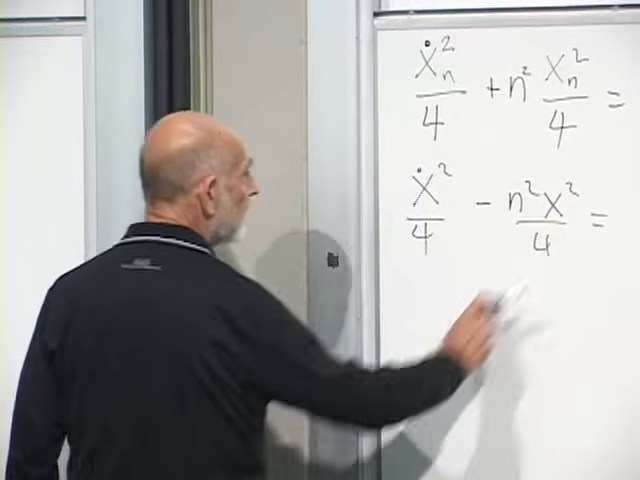
\includegraphics[width=0.82\textwidth]{lecture_03_figure_02.png}
  \caption{黑板上的計算顯示，正則對易關係帶來了\(n\)這個因子。}
  \lectureframe{00:10:30}
  \label{fig:l03-commutator-board}
\end{figure}

\(n\)這個因子告訴我們升降算符應如何歸一化：

\begin{align}
  a_n
  &\equiv
  \frac{\sqrt n}{2}X_n+\frac{i}{\sqrt n}p_n,
  \label{eq:l03-annihilator}\\
  a_n^\dagger
  &\equiv
  \frac{\sqrt n}{2}X_n-\frac{i}{\sqrt n}p_n.
  \label{eq:l03-creator}
\end{align}

它們滿足

\begin{equation}
  [a_n,a_m^\dagger]=\delta_{nm},
  \qquad
  H_n=n\left(a_n^\dagger a_n+\frac12\right).
  \label{eq:l03-oscillator-algebra}
\end{equation}

因此，\(a_n^\dagger\)會在第\(n\)個振子中增加一個量子，但該量子帶有\(n\)個單位的模能量。熟悉的諧振子能階間距並未消失；其頻率為\(\omega_n=n\)。

\begin{figure}[H]
  \centering
  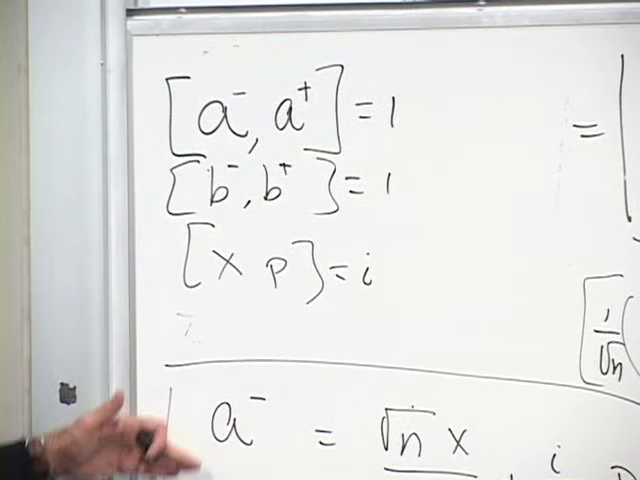
\includegraphics[width=0.82\textwidth]{lecture_03_figure_03.png}
  \caption{第\(n\)個弦振子的歸一化湮滅算符與產生算符。}
  \lectureframe{00:12:00}
  \label{fig:l03-ladder-board}
\end{figure}

\subsection{兩組橫向振子塔}

在四維時空中，沿\(z\)軸帶有極大動量的弦有兩個橫向座標\(X\)和\(Y\)。因此，我們需要兩組彼此獨立的振子塔。令\(a_n,a_n^\dagger\)作用於\(X\)模，\(b_n,b_n^\dagger\)作用於\(Y\)模。由\eqref{eq:l03-annihilator}--\eqref{eq:l03-creator}解出座標，可得

\begin{equation}
  X_n=\frac{a_n+a_n^\dagger}{\sqrt n},
  \qquad
  Y_n=\frac{b_n+b_n^\dagger}{\sqrt n}.
  \label{eq:l03-mode-coordinates}
\end{equation}

\begin{figure}[H]
  \centering
  \includegraphics[width=0.78\textwidth]{lecture_03_figure_04.png}
  \caption{以產生算符與湮滅算符表示模座標。}
  \lectureframe{00:17:05}
  \label{fig:l03-coordinate-operator-board}
\end{figure}

開弦座標以 Neumann 模展開：

\begin{align}
  X(\sigma,\tau)
  &=X_{\rm cm}(\tau)
    +\sum_{n=1}^{\infty}X_n(\tau)\cos(n\sigma),
  \label{eq:l03-X-fourier}\\
  Y(\sigma,\tau)
  &=Y_{\rm cm}(\tau)
    +\sum_{n=1}^{\infty}Y_n(\tau)\cos(n\sigma).
  \label{eq:l03-Y-fourier}
\end{align}

端點斜率為零，因此會出現餘弦。將\eqref{eq:l03-mode-coordinates}代入後，弦本身便成為算符：

\begin{align}
  X(\sigma,\tau)
  &=X_{\rm cm}(\tau)
    +\sum_{n=1}^{\infty}
      \frac{a_n(\tau)+a_n^\dagger(\tau)}{\sqrt n}
      \cos(n\sigma),
  \label{eq:l03-X-operator}\\
  Y(\sigma,\tau)
  &=Y_{\rm cm}(\tau)
    +\sum_{n=1}^{\infty}
      \frac{b_n(\tau)+b_n^\dagger(\tau)}{\sqrt n}
      \cos(n\sigma).
  \label{eq:l03-Y-operator}
\end{align}

\begin{figure}[H]
  \centering
  \begin{minipage}[t]{0.48\textwidth}
    \centering
    \includegraphics[width=\textwidth]{lecture_03_figure_05.png}
    \par\smallskip\footnotesize (a) 座標模展開。
  \end{minipage}\hfill
  \begin{minipage}[t]{0.48\textwidth}
    \centering
    \includegraphics[width=\textwidth]{lecture_03_figure_06.png}
    \par\smallskip\footnotesize (b) 將升降算符代入弦座標。
  \end{minipage}
  \caption{量子開弦的形狀由所有橫向振子算符共同構成。}
  \lectureframe{00:20:35 and 00:21:05}
  \label{fig:l03-string-coordinate-board}
\end{figure}

\begin{classroomqa}
\audiencequestion{\(X_n\)也是\(\sigma\)的函數嗎？\lecturetimestamp{00:21:48}}
\lecturerresponse{不是。對\(\sigma\)的依賴完全包含在\(\cos(n\sigma)\)中。係數\(X_n\)是該空間圖樣隨時間變化的振幅，因此\(X_n=X_n(\tau)\)。}
\end{classroomqa}

\begin{classroomqa}
\audiencequestion{為什麼稱為升算符和降算符的算符，看起來符號卻相反？\lecturetimestamp{00:23:13}}
\lecturerresponse{\(ip_n\)表面上的符號不是命名依據。計算它與哈密頓量的對易子即可判定。滿足\([H_n,a_n^\dagger]=n a_n^\dagger\)的算符會提高能量；滿足\([H_n,a_n]=-n a_n\)的算符則會降低能量。}
\end{classroomqa}

這兩組橫向振子塔是為了教學而採用的四維圖像。一致量子化的玻色弦具有二十六維時空，因此有二十四組橫向振子，而非兩組。以下的論證不變：第一能級態的數目必須與相同維度下無質量向量的物理極化數目相符。

\section{有質量粒子的自旋與無質量粒子的螺旋度}

在替弦態指定自旋之前，我們需要先明確區分兩者。有質量且自旋為\(J\)的粒子具有\(2J+1\)種自旋態，

\begin{equation}
  m_J=-J,-J+1,\ldots,J-1,J.
  \label{eq:l03-massive-spin-multiplet}
\end{equation}

例如，有質量的自旋一粒子有三種極化，有質量的自旋二粒子則有五種。我們可以轉到靜止系來理解原因。在靜止系中，所有空間旋轉都可進行。旋轉自旋軸，再變換回原來的參考系，所有\(2J+1\)個分量都屬於同一個相對論性粒子。

無質量粒子沒有靜止系。它的不變自旋標籤是螺旋度，也就是沿運動方向的角動量。光子只有\(h=+1\)和\(h=-1\)兩種螺旋度；重力子只有\(h=+2\)和\(h=-2\)兩種。純量有一個\(h=0\)態。本講以反射對稱性將兩種螺旋度配成一對。在手徵理論中，單一無質量不可約表示可能只帶有一種螺旋度，因此這種配對是額外的對稱性條件，並非僅由無質量這一性質所導致。\editorialnote{現代小群分類允許只有單一螺旋度的無質量表示。在熟悉的光子與重力子例子中，宇稱或適當補足 CPT 的場內容會提供相反的螺旋度。}

\begin{figure}[H]
  \centering
  \begin{minipage}[t]{0.45\textwidth}
    \centering
    \includegraphics[width=\textwidth]{lecture_03_figure_07.png}
    \par\smallskip\footnotesize (a) 黑板上開始進行的自旋態計數。
  \end{minipage}\hfill
  \begin{minipage}[t]{0.5\textwidth}
    \centering
    \begin{adjustbox}{max width=\linewidth}
    \begin{tabular}{@{}ccc@{}}
      \toprule
      自旋 & 有質量態 & 無質量螺旋度 \\
      \midrule
      \(0\) & \(1\) & \(0\) \\
      \(1\) & \(3\) & \(+1,-1\) \\
      \(2\) & \(5\) & \(+2,-2\) \\
      \bottomrule
    \end{tabular}
    \end{adjustbox}
  \end{minipage}
  \caption{有質量時，靜止系存在，也因此會有中間的自旋投影態。}
  \lectureframe{00:27:40}
  \label{fig:l03-spin-count}
\end{figure}

\subsection{光子的線偏振與圓偏振}

考慮一個沿\(z\)方向運動的光子。它的兩種橫向線偏振為\(\ket{x}\)和\(\ket{y}\)，但它們不是螺旋度本徵態。圓偏振態為

\begin{align}
  \ket{R}
  &=\frac{1}{\sqrt2}\left(\ket{x}+i\ket{y}\right),
  \label{eq:l03-right-circular}\\
  \ket{L}
  &=\frac{1}{\sqrt2}\left(\ket{x}-i\ket{y}\right),
  \label{eq:l03-left-circular}
\end{align}

其螺旋度分別為\(+1\)和\(-1\)；正負號取決於右旋與左旋的命名慣例。線偏振光子是這兩種結果的疊加。它的平均螺旋度可以為零，但螺旋度測量絕不會測得自旋為零的光子。同樣地，

\begin{equation}
  \frac{1}{\sqrt2}\left(\ket{x}+\ket{y}\right)
\end{equation}

只是偏振方向為四十五度的線偏振。

\begin{figure}[H]
  \centering
  \begin{minipage}[t]{0.48\textwidth}
    \centering
    \includegraphics[width=\textwidth]{lecture_03_figure_08.png}
    \par\smallskip\footnotesize (a) 黑板上的圓偏振態。
  \end{minipage}\hfill
  \begin{minipage}[t]{0.48\textwidth}
    \centering
    \begin{adjustbox}{max width=\linewidth}
    \begin{tikzpicture}[>=Latex,scale=0.9]
      \draw[->,thick] (0,0) -- (3.4,0) node[right] {\(z\)};
      \draw[->,blue!70!black,thick] (0,0) -- (0,2.0)
        node[above] {\(x\)};
      \draw[->,orange!85!black,thick] (0,0) -- (-1.4,-1.2)
        node[below left] {\(y\)};
      \draw[red!70!black,thick,->]
        plot[domain=0:320,samples=80]
        ({1.0*cos(\x)},{0.58*sin(\x)+0.4});
      \node[red!70!black] at (1.55,1.25) {circular};
    \end{tikzpicture}
    \end{adjustbox}
  \end{minipage}
  \caption{線偏振提供橫向基底；圓偏振組合則使螺旋度算符對角化。}
  \lectureframe{00:37:45}
  \label{fig:l03-polarization}
\end{figure}

\begin{classroomqa}
\audiencequestion{這和 Stern--Gerlach 實驗中的自旋態分離類似嗎？\lecturetimestamp{00:37:40}}
\lecturerresponse{量子疊加的概念相同，但描述光子時，直接使用的術語是偏振。圓偏振測量可以區分兩種螺旋度；光束中並沒有縱向、自旋為零的光子。}
\end{classroomqa}

自旋為二的重力子也呈現相同的模式。若只考慮自旋，可示意性地寫成

\begin{equation}
  \ket{+2}\sim\ket{+1}\otimes\ket{+1},
  \qquad
  \ket{-2}\sim\ket{-1}\otimes\ket{-1}.
  \label{eq:l03-graviton-helicity}
\end{equation}

這並不是說重力子真的是由兩個光子組成，而是說兩個相同的螺旋度相加後，會得到正確的自旋二螺旋度。

\begin{classroomqa}
\audiencequestion{雙光子的類比也適用於其他量子數嗎？\lecturetimestamp{00:41:05}}
\lecturerresponse{不能把它當作組成模型。有些重要公式會將重力振幅表示為規範理論振幅的乘積，或``平方，''但重力子仍是獨立的粒子。此處最可靠的類比，是把它視為螺旋度的陳述。\editorialnote{現代的 Kawai--Lewellen--Tye 關係與雙重拷貝關係，能在適當的理論中精確描述振幅間的關係；但它們並不會把重力子變成兩個光子的束縛態。}}
\end{classroomqa}

\begin{classroomqa}
\audiencequestion{光子可以有任意動量，因此它的譜不是連續的嗎？粒子所要求的不是孤立的譜嗎？\lecturetimestamp{00:42:17}}
\lecturerresponse{連續變數是質心動量。固定這個動量，再檢視內部的不變質量。粒子由孤立的質量能級來識別；改變粒子的整體動量，則會得到通常的連續色散關係。}
\end{classroomqa}

\section{最低的開弦能級}

現在可以回到弦。在大動量描述中，有限的內部光前能量與不變質量平方成正比。暫略整體的弦尺度，將譜寫成

\begin{equation}
  \begin{aligned}
    M^2
    &=m_0^2
      +\sum_{n=1}^{\infty}n
       \left(N_n^{(a)}+N_n^{(b)}\right),\\
    N_n^{(a)}&=a_n^\dagger a_n,
    \qquad
    N_n^{(b)}=b_n^\dagger b_n.
  \end{aligned}
  \label{eq:l03-open-spectrum}
\end{equation}

振子基態滿足

\begin{equation}
  a_n\ket{0}=0,
  \qquad
  b_n\ket{0}=0,
  \qquad n=1,2,\ldots .
  \label{eq:l03-ground-annihilation}
\end{equation}

這不是弦不存在，而是量子弦的最低激發態；它的座標仍會漲落。令其質量平方為\(m_0^2\)，目前尚未決定。

\begin{figure}[H]
  \centering
  \includegraphics[width=0.78\textwidth]{lecture_03_figure_09.png}
  \caption{開弦基態，以及定義此基態的湮滅條件。}
  \lectureframe{00:45:20}
  \label{fig:l03-ground-state-board}
\end{figure}

能量最低的激發使用\(n=1\)產生算符：

\begin{equation}
  a_1^\dagger\ket{0},
  \qquad
  b_1^\dagger\ket{0},
  \qquad
  M^2=m_0^2+1.
  \label{eq:l03-first-level}
\end{equation}

\begin{figure}[H]
  \centering
  \includegraphics[width=0.78\textwidth]{lecture_03_figure_10.png}
  \caption{兩個簡併的第一能級態之一；黑板上也寫出了它的質量平方增量。}
  \lectureframe{00:49:25}
  \label{fig:l03-first-level-board}
\end{figure}

「``一''」在式{eq:l03-first-level}中並非一焦耳、一電子伏特或一普朗克質量。我們省略了有量綱的弦尺度。目前它表示振子的質量平方階梯上的一個步階；缺少的單位將在下一堂課補回。

這兩個簡併態的任意線性組合也都是此能級上的態。特別是，

\begin{equation}
  \frac{1}{\sqrt2}
  \left(a_1^\dagger\pm i b_1^\dagger\right)\ket{0}
  \label{eq:l03-string-circular-states}
\end{equation}

這是弦的圓偏振類比。在\(x\)-\(y\)平面內旋轉時，\(a_1^\dagger\)和\(b_1^\dagger\)的變換方式如同橫向向量的兩個分量。因此，\eqref{eq:l03-string-circular-states}中的組合具有螺旋度\(+1\)和\(-1\)。

\begin{figure}[H]
  \centering
  \includegraphics[width=0.82\textwidth]{lecture_03_figure_11.png}
  \caption{黑板上整理了基態條件、兩個第一能級激發態，以及它們的圓偏振組合。}
  \lectureframe{00:56:00}
  \label{fig:l03-level-structure-board}
\end{figure}

沒有第三個簡併態可作為縱向極化。如果這兩個態有非零質量，則自旋一的相對論性粒子需要三種極化。但這裡恰好只有兩種，因此此態必須是無質量的。於是

\begin{equation}
  m_0^2+1=0,
  \qquad
  m_0^2=-1.
  \label{eq:l03-intercept-condition}
\end{equation}

第一能級具有光子般的性質：它是無質量的規範向量態，但不一定是電磁學中的光子；它最終對應哪種規範場，取決於弦模型。其下方的基態具有負質量平方，這就是玻色開弦的快子。\editorialnote{在完整的臨界玻色弦中，正規序截距與洛侖茲代數都和\(D=26\)有關。本講只考慮兩個橫向方向，是同一套態計數論證在四維中的呈現：\(D-2\)個第一能級振子態，恰與無質量向量的\(D-2\)個物理極化相符。}

\begin{classroomqa}
\audiencequestion{為什麼我們需要在意\(m_0^2\)是負的？\lecturetimestamp{00:56:35}}
\lecturerresponse{因為質量平方代表二次場勢在我們稱為真空的態附近的曲率。曲率為負，表示這個構型不是穩定的基態。接下來的計算會將此說法表達得更精確。}
\end{classroomqa}

\section{快子的真正意義}

``快子''這個名稱容易讓人一開始就產生誤解。先從\(c=1\)的相對論色散關係出發，

\begin{equation}
  E(p)=\sqrt{p^2+m^2}.
  \label{eq:l03-relativistic-dispersion}
\end{equation}

對於波包，群速度為

\begin{equation}
  v_g=\frac{dE}{dp}.
  \label{eq:l03-group-velocity}
\end{equation}

這會得到熟悉的情形：

\begin{align}
  E_{\rm nr}(p)&=\frac{p^2}{2m},
  &v_g&=\frac{p}{m},
  \label{eq:l03-nr-group-velocity}\\
  E_\gamma(p)&=|p|,
  &|v_g|&=1,
  \label{eq:l03-photon-group-velocity}\\
  E_m(p)&=\sqrt{p^2+m^2},
  &|v_g|&=\frac{|p|}{\sqrt{p^2+m^2}}<1.
  \label{eq:l03-massive-group-velocity}
\end{align}

\begin{figure}[H]
  \centering
  \begin{minipage}[t]{0.48\textwidth}
    \centering
    \includegraphics[width=\textwidth]{lecture_03_figure_12.png}
    \par\smallskip\footnotesize (a) 非相對論性的群速度。
  \end{minipage}\hfill
  \begin{minipage}[t]{0.48\textwidth}
    \centering
    \includegraphics[width=\textwidth]{lecture_03_figure_13.png}
    \par\smallskip\footnotesize (b) 相對論性色散關係及其導數。
  \end{minipage}
  \caption{由\(E(p)\)的斜率讀出傳播速度。}
  \lectureframe{01:01:50 and 01:03:15}
  \label{fig:l03-group-velocity-board}
\end{figure}

若\(m^2=-\mu^2\)，形式上便得到

\begin{equation}
  E(p)=\sqrt{p^2-\mu^2},
  \qquad
  v_g=\frac{p}{\sqrt{p^2-\mu^2}},
  \label{eq:l03-formal-tachyon-dispersion}
\end{equation}

只要平方根內的量為實數，就有\(|v_g|>1\)。但這並非玻色弦基態的正確物理解釋。低動量時頻率已是虛數，問題在此便已顯現。

\subsection{場勢的負曲率}

考慮一維空間中的實純量場，

\begin{equation}
  \left(\partial_t^2-\partial_x^2+m^2\right)\phi=0.
  \label{eq:l03-klein-gordon}
\end{equation}

對於平面波\(\phi\propto e^{-i\omega t+ikx}\)，

\begin{equation}
  \omega^2=k^2+m^2.
  \label{eq:l03-kg-dispersion}
\end{equation}

\begin{figure}[H]
  \centering
  \includegraphics[width=0.82\textwidth]{lecture_03_figure_14.png}
  \caption{用來揭示負質量平方所導致不穩定性的 Klein--Gordon 方程。}
  \lectureframe{01:06:40}
  \label{fig:l03-klein-gordon-board}
\end{figure}

守恆的二次能量為

\begin{equation}
  \mathcal E
  =\frac12\int dx\,
  \left[
    \dot\phi^{\,2}
    +(\partial_x\phi)^2
    +m^2\phi^2
  \right].
  \label{eq:l03-field-energy}
\end{equation}

\begin{figure}[H]
  \centering
  \includegraphics[width=0.82\textwidth]{lecture_03_figure_15.png}
  \caption{純量場的能量，其中質量項決定勢能在局部的曲率。}
  \lectureframe{01:08:10}
  \label{fig:l03-field-energy-board}
\end{figure}

當\(m^2>0\)時，局部勢能\(V(\phi)=\tfrac12m^2\phi^2\)呈碗狀，構型\(\phi=0\)位於碗底。若\(m^2=-\mu^2\)，同一點便是倒置碗狀勢能的頂端。方程\eqref{eq:l03-kg-dispersion}變為

\begin{equation}
  \omega^2=k^2-\mu^2.
  \label{eq:l03-tachyonic-modes}
\end{equation}

對於\(k^2<\mu^2\)的模，

\begin{equation}
  \omega=\pm i\sqrt{\mu^2-k^2},
  \qquad
  \phi_k(t)\propto
  e^{\pm\sqrt{\mu^2-k^2}\,t}.
  \label{eq:l03-growing-mode}
\end{equation}

其中一個分支會指數增長。因此，所謂的真空並不穩定：任意微小的長波長擾動都會使場偏離\(\phi=0\)。這就是譜中出現快子的意義。

\subsection{倒立擺鏈}

一排彼此耦合的擺能清楚呈現這個差異。讓每個擺都保持直立。這個均勻構型確實存在，但它在勢能極大值處達到平衡。只要輕推其中一個擺，它就會倒下並牽動鄰近的擺。倒下的前沿會以耦合所決定的有限訊號速度沿著鏈傳播。

\begin{figure}[H]
  \centering
  \begin{minipage}[t]{0.48\textwidth}
    \centering
    \includegraphics[width=\textwidth]{lecture_03_figure_16.png}
    \par\smallskip\footnotesize (a) 黑板上的耦合直立擺模型。
  \end{minipage}\hfill
  \begin{minipage}[t]{0.48\textwidth}
    \centering
    \begin{adjustbox}{max width=\linewidth}
    \begin{tikzpicture}[>=Latex,scale=0.78]
      \draw[thick] (-0.3,0) -- (6.3,0);
      \foreach \x/\a in {0/0,1/0,2/8,3/28,4/55,5/72,6/78}{
        \fill (\x,0) circle (0.06);
        \draw[thick] (\x,0) -- ++({90-\a}:1.25);
        \fill[blue!65!black]
          ($(\x,0)+({90-\a}:1.25)$) circle (0.11);
      }
      \draw[red!70!black,->,thick] (1.7,-0.45) -- (4.6,-0.45)
        node[midway,below] {falling front};
    \end{tikzpicture}
    \end{adjustbox}
  \end{minipage}
  \caption{即使系統的線性化譜包含負質量平方，不穩定性仍會以符合因果律的方式傳播。}
  \lectureframe{01:10:40}
  \label{fig:l03-pendulum-instability}
\end{figure}

這個機制不允許任何受控訊號超越因果前沿。快子模指出的是錯誤的展開點，而不是穩定的超光速訊息載體。\editorialnote{對於局域相對論性場方程，前沿速度仍是因果速度。實數的高\(k\)分支所具有的形式群速度，並不會讓不穩定真空成為超光速通訊通道。}

\begin{classroomqa}
\audiencequestion{剛才找到的無質量態，就是弦理論所預言的重力子嗎？\lecturetimestamp{01:14:27}}
\lecturerresponse{不是。它是開弦的自旋一態，具有兩種極化，因此類似規範玻色子。重力子則是閉弦的自旋二激發態。}
\end{classroomqa}

\begin{classroomqa}
\audiencequestion{倒置的勢在數學上可以成立嗎？系統倒下後會停在哪裡？\lecturetimestamp{01:15:17}}
\lecturerresponse{這完全可以作為局部近似，但單靠這個近似並沒有基態，因為能量沒有下界。更完整的勢能可能會再次向上彎曲，並具有更低的極小值。接著，系統會朝那個穩定構型滾落或凝聚。}
\end{classroomqa}

普通玻色弦正有這個缺陷。較高的振子態仍屬於譜的一部分，但它們是建立在不穩定背景上的激發態。一致的超弦理論會在穩定扇區中排除開弦快子，同時保留無質量與有質量的弦激發態。

\begin{classroomqa}
\audiencequestion{除了兩種極化之外，這個開弦態的其他性質也和光子相符嗎？\lecturetimestamp{01:17:07}}
\lecturerresponse{這個態的行為如同無質量規範玻色子。它具體的電荷指派、輻射規則與粒子身分都取決於弦模型，因此應稱它為類光子態，而不宜立刻認定它就是電磁作用中的光子。這些交互作用性質會在後續討論。}
\end{classroomqa}

\section{弦的交互作用}

自由弦的譜只涵蓋理論的一半，弦也會結合與分裂。首先可以先記住，激發態的自由弦能帶有角動量。一根筆直的旋轉弦會繞著質心轉動，其能量與角動量會沿著熟知的弦狀軌跡一同增加。

\begin{figure}[H]
  \centering
  \includegraphics[width=0.72\textwidth]{lecture_03_figure_17.png}
  \caption{以質心為中心旋轉的開弦示意圖。}
  \lectureframe{01:19:30}
  \label{fig:l03-rotating-string-board}
\end{figure}

\begin{classroomqa}
\audiencequestion{自由弦能以一個固定端點為軸，端對端地旋轉嗎？\lecturetimestamp{01:20:02}}
\lecturerresponse{沒有錨定物就不行。自由的孤立系統會繞質心旋轉。如果一個端點連接到另一個物體或膜上，整個系統便能繞不同的中心旋轉；就像電子和原子核繞著共同質心運行，但質量大得多的原子核看起來幾乎固定不動。}
\end{classroomqa}

\subsection{開弦頂點}

對開弦而言，基本交互作用發生於兩個端點在同一時空點相遇之時。兩端點結合成一條弦的振幅為\(g_s\)。反向演化則對應一條弦分裂成兩條弦的振幅。示意如下：

\begin{equation}
  \text{open}+\text{open}
  \quad\rightleftarrows\quad
  \text{open}.
  \label{eq:l03-open-joining}
\end{equation}

\begin{figure}[H]
  \centering
  \begin{minipage}[t]{0.48\textwidth}
    \centering
    \includegraphics[width=\textwidth]{lecture_03_figure_18.png}
    \par\smallskip\footnotesize 黑板上的結合過程。
  \end{minipage}\hfill
  \begin{minipage}[t]{0.48\textwidth}
    \centering
    \begin{tikzpicture}[>=Latex,scale=0.9]
      \draw[->] (0,-2.1) -- (0,2.2) node[above] {time};
      \draw[blue!70!black,thick] (-2,-1.6) .. controls (-1.3,-0.9)
        and (-0.7,-0.35) .. (0,0);
      \draw[blue!70!black,thick] (2,-1.6) .. controls (1.3,-0.9)
        and (0.7,-0.35) .. (0,0);
      \draw[orange!85!black,thick] (0,0) .. controls (0.25,0.7)
        and (-0.15,1.25) .. (0.15,1.9);
      \fill[red!70!black] (0,0) circle (0.09);
      \node[right] at (0.12,0) {\(g_s\)};
    \end{tikzpicture}
  \end{minipage}
  \caption{端點結合是弦的局域粒子交互作用頂點；時間反演則對應分裂。}
  \lectureframe{01:24:05}
  \label{fig:l03-open-vertex}
\end{figure}

耦合是振幅。對於某個指定的基本過程，其相應機率的最低階項為\(|g_s|^2\)；相空間與歸一化因子則由完整計算給出。因此，將\(g_s\)稱為``機率''只是一種非正式的簡稱；區分振幅與機率，才能避免錯誤地多取一次平方。

交互作用的形式不取決於外部弦當下是在振動、旋轉，或處於其他振子態。這些態會改變矩陣元的細節，但採用的仍是同一種局域結合規則。

\subsection{開弦可以自行閉合}

假設一條開弦的兩個端點相遇。結合規則無法辨別它們是否屬於同一條弦，因此兩端點可以融合，形成一個閉合環：

\begin{equation}
  \text{open}\longrightarrow\text{closed}.
  \label{eq:l03-self-closing}
\end{equation}

\begin{figure}[H]
  \centering
  \begin{minipage}[t]{0.48\textwidth}
    \centering
    \includegraphics[width=\textwidth]{lecture_03_figure_19.png}
    \par\smallskip\footnotesize (a) 開弦讓兩個端點彼此靠近。
  \end{minipage}\hfill
  \begin{minipage}[t]{0.48\textwidth}
    \centering
    \begin{tikzpicture}[>=Latex,scale=0.92]
      \draw[blue!70!black,thick]
        (-2,0) .. controls (-1.2,1.5) and (1.2,1.5) .. (2,0);
      \fill[red!70!black] (-2,0) circle (0.08);
      \fill[red!70!black] (2,0) circle (0.08);
      \draw[->,thick] (-0.45,-0.45) -- (0.45,-0.45);
      \draw[orange!85!black,thick] (0,-1.55) ellipse (1.15 and 0.58);
      \node at (0,-2.25) {closed string};
    \end{tikzpicture}
  \end{minipage}
  \caption{有交互作用的開弦必然會產生閉弦。}
  \lectureframe{01:27:20}
  \label{fig:l03-open-becomes-closed}
\end{figure}

這並非可有可無的額外內容。任何包含開弦交互作用的理論都必須包含閉弦態。反向過程則允許閉弦在具備適當的端點與邊界條件時轉變為開弦。

\begin{classroomqa}
\audiencequestion{弦融合或分裂時，它們的振子能量會改變嗎？理論會決定能量如何改變嗎？\lecturetimestamp{01:28:05}}
\lecturerresponse{會。整個過程的能量與動量都守恆，而激發能則可以在出射弦之間重新分配。躍遷振幅由交互作用頂點與外部波函數決定。}
\end{classroomqa}

\subsection{閉弦之間的交互作用不必產生開弦}

這種推論只適用於單一方向：有交互作用的開弦需要閉弦，但理論可以只從閉弦開始。兩個閉合環可以接觸、重新連接，並合併成一個閉合環；反向過程則會使一個環分裂成兩個。整個過程不需要出現開弦端點。

\begin{figure}[H]
  \centering
  \begin{minipage}[t]{0.48\textwidth}
    \centering
    \includegraphics[width=\textwidth]{lecture_03_figure_20.png}
    \par\smallskip\footnotesize 黑板上的閉弦融合過程。
  \end{minipage}\hfill
  \begin{minipage}[t]{0.48\textwidth}
    \centering
    \begin{tikzpicture}[>=Latex,scale=0.88]
      \draw[blue!70!black,thick] (-1.35,0) circle (0.75);
      \draw[blue!70!black,thick] (1.35,0) circle (0.75);
      \draw[->,thick] (-0.35,-1.15) -- (0.35,-1.15);
      \draw[orange!85!black,thick] (0,-2.3) ellipse (1.35 and 0.68);
      \node at (0,1.2) {closed \(+\) closed};
      \node at (0,-3.25) {closed};
    \end{tikzpicture}
  \end{minipage}
  \caption{閉弦有自己的結合與分裂交互作用，不必經過開弦態。}
  \lectureframe{01:29:05}
  \label{fig:l03-closed-fusion}
\end{figure}

\begin{classroomqa}
\audiencequestion{若理論以閉弦為起點，也必須包含開弦嗎？\lecturetimestamp{01:28:35}}
\lecturerresponse{不必。閉弦可以透過重新連接彼此交互作用，並在整個過程中保持閉合。開弦則需要額外的邊界資料，例如允許的端點或膜。}
\end{classroomqa}

\section{為什麼引力無可避免}

閉弦振子的計算與開弦相似，但閉弦具有彼此獨立的左行與右行激發。兩者最低的非平凡匹配能級中包含無質量的自旋二態，其螺旋度正是重力子的螺旋度。因此，每個一致的閉弦交互作用理論都包含引力。

\begin{classroomqa}
\audiencequestion{為什麼最低的閉弦激發態必定是重力子，就像開弦能級必定是類光子態一樣？
\lecturetimestamp{01:30:59}}
\lecturerresponse{答案是同一類型的態計數，不過現在考慮的是左行與右行振子向量。它們的張量積包含無質量、對稱且無跡的自旋二極化態。下一講會詳細推導閉弦的譜；目前的重點是這個態的存在無可避免。}
\end{classroomqa}

開弦與閉弦也能彼此交互作用。閉環可以與開弦相遇並被吸收，使開弦變得更長，或轉變成不同的激發態。反過來，開弦也可以放射出閉環。在粒子層次上，這代表物質發射或吸收重力子。

\begin{figure}[H]
  \centering
  \begin{minipage}[t]{0.48\textwidth}
    \centering
    \includegraphics[width=\textwidth]{lecture_03_figure_21.png}
    \par\smallskip\footnotesize 弦段的局域重新連接。
  \end{minipage}\hfill
  \begin{minipage}[t]{0.48\textwidth}
    \centering
    \includegraphics[width=\textwidth]{lecture_03_figure_22.png}
    \par\smallskip\footnotesize 閉環連接到開弦上。
  \end{minipage}
  \caption{混合開--閉弦交互作用的黑板圖示，以及重力子交換普遍可能存在的原因。}
  \lectureframe{01:33:10 and 01:34:35}
  \label{fig:l03-mixed-interactions-board}
\end{figure}

\begin{figure}[H]
  \centering
  \begin{tikzpicture}[>=Latex,scale=0.88]
    \draw[blue!70!black,thick]
      (-3,-0.5) .. controls (-1.7,-0.1) and (-0.8,0.2) .. (0,0);
    \draw[blue!70!black,thick]
      (0,0) .. controls (0.9,0.3) and (2.0,0.1) .. (3,0.55);
    \draw[orange!85!black,thick] (-0.8,1.55) ellipse (0.75 and 0.45);
    \draw[->,red!70!black,thick] (-0.45,1.15) -- (-0.05,0.35);
    \node[blue!70!black] at (-2.2,-0.95) {open string};
    \node[orange!85!black] at (-0.8,2.25) {closed string};
    \node at (1.75,-0.5) {excited open string};
  \end{tikzpicture}
  \caption{不含時空背景的閉弦被開弦吸收之示意圖。}
  \label{fig:l03-mixed-interaction-redraw}
\end{figure}

每種弦態都能與重力子耦合，因為每條弦都帶有能量與動量，而且結合規則允許閉弦交換。這就是弦理論中引力具有普適性的由來。

\begin{classroomqa}
\audiencequestion{閉弦能轉變成開弦嗎？或者，它能在不違反端點規則的情況下與開弦結合嗎？\lecturetimestamp{01:31:20}}
\lecturerresponse{若理論同時包含這兩種扇區，閉弦可以附著到開弦上並改變開弦的狀態。單獨一條閉弦能否直接轉變成開弦，則取決於理論是否提供了合乎條件的端點。局域重新連接規則仍然相同。}
\end{classroomqa}

\begin{classroomqa}
\audiencequestion{閉合弦圈能否永久地彼此連結或打結？\lecturetimestamp{01:35:10}}
\lecturerresponse{在弱耦合下，弦大多近乎透明：除非微小的重聯振幅發揮作用，否則它們可以彼此穿過。因此，連結或結可以維持一段時間，但在允許的弦相互作用發生時，拓撲便可能改變。}
\end{classroomqa}

\begin{classroomqa}
\audiencequestion{相互作用機率是否與弦的狀態或速度無關？\lecturetimestamp{01:36:09}}
\lecturerresponse{局域耦合是同一個參數，但總躍遷機率也取決於波函數，以及相關部分彼此接觸的時間長短。快速相遇通常比緩慢相遇提供較短的相互作用時間。}
\end{classroomqa}

\section{仍未補上的尺度與耦合}

有兩項量綱上的處理刻意先擱置。第一，\(X\) 是長度，而 \(a_n\) 是無量綱的，因此 \eqref{eq:l03-mode-coordinates} 中的比例關係必須包含一個長度尺度。第二，振子能級提高時，不可能真的把一個無量綱數加到物理質量平方上。補回弦長 \(\ell_s\)，或等價地補回 Regge 斜率 \(\alpha'\sim\ell_s^2\)，就能補上缺少的量綱：

\begin{equation}
  M^2\sim\frac{1}{\alpha'}(N-a).
  \label{eq:l03-dimensional-spectrum}
\end{equation}

精確的約定與正規化將在下一講中確定。

\begin{classroomqa}
\audiencequestion{弦長的尺度，以及一個產生算符所增加的質量，由什麼決定？\lecturetimestamp{01:37:03}}
\lecturerresponse{有一個帶量綱的常數被省略了。它就是弦尺度，通常寫作 \(\ell_s\) 或 \(\alpha'\)。振子算符是無量綱的；弦尺度的冪次會將振子的能級數轉換為物理長度、張力與質量平方。}
\end{classroomqa}

第二個參數是弦耦合 \(g_s\)。在最簡單的討論中，它是一個控制弦的結合與分裂的普適數值。在較豐富的模型中，端點可以帶有不同標記，弦也可以在交會處相接。Y 形構型是三條通量管相遇的弦論類比；在早期的強子圖像中，它與三夸克重子相關，而一段單獨的開弦則類似夸克--反夸克介子。

\begin{classroomqa}
\audiencequestion{不同的弦端點能否有不同的結合機率？\lecturetimestamp{01:39:31}}
\lecturerresponse{最簡單的模型採用單一耦合。更精細的理論會在端點上附加荷或邊界標記，再由選擇定則決定哪些結合過程允許發生。詳細構造留待之後討論，但普適的局域結合概念仍然成立。}
\end{classroomqa}

\begin{classroomqa}
\audiencequestion{弦能否沿長度方向分裂，或形成 Y 形交會？\lecturetimestamp{01:40:01}}
\lecturerresponse{某些弦系統確實允許交會。這不是剛才所畫的普通雙端點分裂過程；只有當理論具有相容的弦荷時，才會出現這類交會。介子--重子通量管的類比有助於理解兩者的區別。}
\end{classroomqa}

\begin{classroomqa}
\audiencequestion{改變時空維度會改變相互作用耦合嗎？\lecturetimestamp{01:42:25}}
\lecturerresponse{維度會改變譜、相空間，以及緊緻化後得到的有效耦合。基本弦耦合仍然決定微擾展開的組織方式，但它在低維理論中的表現取決於額外維度的幾何與體積。}
\end{classroomqa}

\begin{classroomqa}
\audiencequestion{自由弦一開始運動，是由引力造成的嗎？\lecturetimestamp{01:43:17}}
\lecturerresponse{維持運動不需要力。初始位置與速度決定一個自由解；慣性使弦持續運動。引力或其他力會改變它的運動。追問初始條件由何而來，是另一個問題，不屬於局域運動方程的一部分。}
\end{classroomqa}

因此，我們得到三個彼此相關的結論。將開弦量子化，會在第一激發能級得到一個無質量向量；位於其下的玻色弦基態是不穩定的；而弦的相互作用必然會引入閉弦，其譜中包含引力。接下來要補回缺少的尺度，並明確地進行閉弦量子化。
\chapter{閉弦、能階匹配與對偶性}

\lectureoverview{閉弦沿著兩個內在方向各自承載獨立的波。將這些波量子化，乍看之下似乎會使開弦的光子數加倍，但弦座標原點平移下的不變性會排除只存在於單一方向的狀態。第一個留下的能階含有一個無質量自旋二粒子。改變描述方式的同一個想法，接著引出一個更廣泛的問題：耦合變化時，稱任何物件為基本的究竟有什麼意義？}

\section{留待後用的生成元}

在畫出閉弦之前，先回顧一個正則力學的結果。設
\begin{equation}
  L=L(q_i,\dot q_i),
\end{equation}
並將與 \(q_i\) 共軛的動量定義為
\begin{equation}
  p_i=\frac{\partial L}{\partial\dot q_i}.
\end{equation}
無窮小連續變換可寫成
\begin{equation}
  \delta q_i=\epsilon f_i(q),
  \label{eq:l04-infinitesimal-transformation}
\end{equation}
其中 \(\epsilon\) 是一個小參數。若此變換是對稱性，諾特定理便會給出守恆荷。將座標位移除以共同參數，就得到生成元
\begin{equation}
  Q=\sum_i p_i f_i(q)
   =\frac{1}{\epsilon}\sum_i p_i\,\delta q_i.
  \label{eq:l04-noether-charge}
\end{equation}
在量子力學中，\(Q\) 是生成相應無窮小變換的算符。

在 \(xy\) 平面上的旋轉是個熟悉的例子。採用其中一種取向約定，
\begin{equation}
  \delta x=\epsilon y,
  \qquad
  \delta y=-\epsilon x,
\end{equation}
而 \eqref{eq:l04-noether-charge} 就是角動量，至多差一個相同的符號約定。這個具體例子並不重要；重要的是其一般形式：動量與無窮小位移縮並，便得到生成元。

\begin{figure}[H]
  \centering
  \includegraphics[width=0.76\textwidth]{lecture_04_figure_01.png}
  \caption{為稍後平移閉弦座標時保留的正則動量與諾特生成元。}
  \lectureframe{00:05:00}
  \label{fig:l04-noether-board}
\end{figure}

我們很快會遇到一種對稱性，其座標不是普通空間中的點，而是弦上各點的標記。式 \eqref{eq:l04-noether-charge} 正是為此預先備妥的。

\section{環繞一圈的座標}

閉弦沒有端點。選取一個參數
\begin{equation}
  0\leq \sigma<2\pi
\end{equation}
並暫時將其中一點標記為 \(\sigma=0\)。繞行半圈的位置是 \(\sigma=\pi\)；四分之一圈與四分之三圈的位置分別是 \(\pi/2\) 和 \(3\pi/2\)。這個標記建立的是座標約定，尚非物理特徵。

\begin{figure}[H]
  \centering
  \begin{minipage}[t]{0.58\textwidth}
    \centering
    \includegraphics[width=\textwidth]{lecture_04_figure_02.png}
    \par\smallskip\footnotesize (a) 黑板上標出記號的圈。
  \end{minipage}\hfill
  \begin{minipage}[t]{0.37\textwidth}
    \centering
    \begin{adjustbox}{max width=\linewidth}
    \begin{tikzpicture}[scale=0.82]
      \draw[thick]
        (0.1,1.1)
        .. controls (1.0,1.55) and (2.4,1.45) .. (2.9,0.4)
        .. controls (3.25,-0.45) and (2.45,-1.35) .. (1.55,-1.05)
        .. controls (0.65,-1.45) and (-0.35,-1.0) .. (-0.35,-0.05)
        .. controls (-0.35,0.55) and (-0.05,0.9) .. (0.1,1.1);
      \fill (0.1,1.1) circle (1.8pt);
      \node[above] at (0.1,1.12) {\(\sigma=0\)};
      \draw[->,thick] (2.55,0.95) arc[start angle=42,end angle=-25,radius=0.62];
      \node[right] at (3.05,0.55) {increasing \(\sigma\)};
    \end{tikzpicture}
    \end{adjustbox}
    \par\smallskip\footnotesize (b) 內在取向。
  \end{minipage}
  \caption{標記一點以定義原點，並以箭頭標示 \(\sigma\) 增大的方向。}
  \lectureframe{00:06:48}
  \label{fig:l04-closed-string-origin}
\end{figure}

沿著圈的箭頭表示一種\emph{內在}取向。不可將它與 \(xy\) 平面上的順時針或逆時針運動混為一談。想像將一條標了記號的橡皮筋從黑板上拿起、翻面，再放回去。它表面上的順時針方向會反轉，但內在記號的排列順序不變。\(\sigma\) 增大的方向仍然是 \(\sigma\) 增大的方向。

這項區分決定了右行波與左行波的用法。在本章中，右行擾動指沿著 \(\sigma\) 增大的方向傳播的擾動，左行擾動則指沿著 \(\sigma\) 減小的方向傳播的擾動。這兩個名稱都不表示擾動在房間裡看起來朝哪個方向移動。

在早期強子弦圖像中，取向曾扮演具體角色。將一條有取向的通量管斷開，會在一端產生夸克，在另一端產生反夸克；內在箭頭可區分這兩端。也可以建構無取向的弦理論，但在此處的討論中，我們保留箭頭以及沿箭頭的兩個方向。

\section{週期性與行波}

令 \(X(\sigma,\tau)\) 和 \(Y(\sigma,\tau)\) 為弦的兩個橫向座標，並以 \(\tau\) 表示時間。若還有其他橫向座標，處理方式也完全相同。由於 \(\sigma=0\) 和 \(\sigma=2\pi\) 標記的是同一點，
\begin{equation}
  X(\sigma+2\pi,\tau)=X(\sigma,\tau),
  \qquad
  Y(\sigma+2\pi,\tau)=Y(\sigma,\tau).
  \label{eq:l04-periodicity}
\end{equation}

\begin{figure}[H]
  \centering
  \includegraphics[width=0.76\textwidth]{lecture_04_figure_03.png}
  \caption{兩個橫向座標的週期性邊界條件。}
  \lectureframe{00:12:40}
  \label{fig:l04-periodicity-board}
\end{figure}

因此，局部擾動可以不斷繞圈傳播。抵達 \(2\pi\) 時，它會直接在 \(0\) 再度出現。這與開弦不同：行波抵達端點後會反射，原本左行的波變成右行，反之亦然。駐波適用於開弦，而閉弦則容許兩個彼此獨立傳播的波族。

\subsection{複數傅立葉模態}

週期函數的一組方便基底是
\begin{equation}
  e^{in\sigma}=\cos(n\sigma)+i\sin(n\sigma),
  \qquad n\in\mathbb Z.
\end{equation}
週期性要求指標為整數：
\(e^{in(\sigma+2\pi)}=e^{in\sigma}\)。例如，若將 \(n\) 換成半整數，函數在繞行一圈後就會改變。

暫時略去時間依賴後，黑板上的展開式為
\begin{align}
  X(\sigma)
  &=
  X_0+
  \sum_{n>0}X_n e^{in\sigma}
  +\sum_{n>0}X_{-n}e^{-in\sigma},
  \label{eq:l04-fourier-x}\\
  Y(\sigma)
  &=
  Y_0+
  \sum_{n>0}Y_n e^{in\sigma}
  +\sum_{n>0}Y_{-n}e^{-in\sigma}.
  \label{eq:l04-fourier-y}
\end{align}
在經典層次上，若 \(X\) 和 \(Y\) 為實數，負指標的係數便是相應正指標係數的複共軛。零模 \(X_0\) 和 \(Y_0\) 指定質心的位置；它們是位置，不是內部振動。

\begin{figure}[H]
  \centering
  \includegraphics[width=0.82\textwidth]{lecture_04_figure_04.png}
  \caption{週期傅立葉展開中正指標與負指標的部分，以及零模。}
  \lectureframe{00:20:00}
  \label{fig:l04-fourier-board}
\end{figure}

\begin{classroomqa}
\audiencequestion{如果這些是行波，時間座標在哪裡？\lecturetimestamp{00:19:05}}
\lecturerresponse{它只是在黑板記號中暫時省略了。行波解的相位同時包含 \(\sigma\) 和 \(\tau\)。採用下文的約定，其中一個波族的相位是
\(e^{-in(\tau-\sigma)}\)，另一個則是
\(e^{-in(\tau+\sigma)}\)。}
\end{classroomqa}

因此，決定傳播方向的是完整相位，而不是單看純空間傅立葉因子中 \(n\) 的正負號。我們可以寫成
\begin{equation}
  X(\sigma,\tau)=X_R(\tau-\sigma)+X_L(\tau+\sigma),
  \label{eq:l04-chiral-solution}
\end{equation}
對 \(Y\) 也可作同樣表示。將哪一族稱為 \(R\)、哪一族稱為 \(L\)，只是約定；不變的事實是，沿著 \(\sigma\) 圓有兩個相反的方向。\editorialnote{\(e^{in\sigma}\) 這個因子在某一瞬間本身並不足以指定行波。必須給定時間相位，才能確定傳播方向。}

\section{兩個方向上的能量}

局部動力學與開弦相同。在此採用的簡化歸一化下，
\begin{equation}
  L\propto
  \int_0^{2\pi}d\sigma\,
  \left[
    \dot X^2-X'^2+\dot Y^2-Y'^2
  \right],
  \label{eq:l04-string-lagrangian}
\end{equation}
其中點號表示 \(\partial_\tau\)，撇號表示 \(\partial_\sigma\)。動能項與彈性項在能量中以正號相加：
\begin{equation}
  E\propto
  \int_0^{2\pi}d\sigma\,
  \left[
    \dot X^2+X'^2+\dot Y^2+Y'^2
  \right].
  \label{eq:l04-string-energy}
\end{equation}
對任一橫向座標，
\begin{equation}
  \dot X^2+X'^2
  =
  \frac12(\dot X+X')^2+
  \frac12(\dot X-X')^2.
  \label{eq:l04-energy-square-completion}
\end{equation}
交叉項會相消，恰好留下原有的動能與梯度能。

\begin{figure}[H]
  \centering
  \includegraphics[width=0.82\textwidth]{lecture_04_figure_05.png}
  \caption{總能量重新整理為兩個行波扇區的能量。}
  \lectureframe{00:25:10}
  \label{fig:l04-energy-board}
\end{figure}

對 \(X_R(\tau-\sigma)\)，有 \(\dot X_R=-X_R'\)；對 \(X_L(\tau+\sigma)\)，則有 \(\dot X_L=X_L'\)。因此，\eqref{eq:l04-energy-square-completion} 中的兩個平方項分別挑出兩個手徵波族。將所有橫向座標都納入，定義
\begin{align}
  E_L&\propto
  \frac12\int_0^{2\pi}d\sigma
  \sum_I(\dot X^I+X^{I\prime})^2,\\
  E_R&\propto
  \frac12\int_0^{2\pi}d\sigma
  \sum_I(\dot X^I-X^{I\prime})^2.
  \label{eq:l04-left-right-energies}
\end{align}
於是 \(E=E_L+E_R\)。此時方程是線性的，因此兩個扇區的波會彼此交錯通過而不發生散射。

\subsection{振子數加倍}

將傅立葉級數代入 \eqref{eq:l04-string-lagrangian}，每個非零模態係數都會成為一個諧振子。其頻率正比於 \(|n|\)：波長越短，頻率越高，激發能也越大。不同於開弦，每個正頻率都有兩個獨立傳播的副本。

黑板上將 \(X\) 極化的產生算符標記為 \(a_n^+\) 和 \(a_{-n}^+\)，將 \(Y\) 極化的產生算符標記為 \(b_n^+\) 和 \(b_{-n}^+\)。為了更清楚地區分產生算符與傳播方向，我們採用記號
\begin{equation}
  a_n^\dagger,\quad b_n^\dagger,
  \qquad
  \widetilde a_n^\dagger,\quad\widetilde b_n^\dagger,
  \qquad n>0.
  \label{eq:l04-oscillator-notation}
\end{equation}
不帶波浪號與帶波浪號的算符分別產生沿世界面相反方向傳播的振子；\(a\) 和 \(b\) 表示兩個橫向極化。

\begin{figure}[H]
  \centering
  \includegraphics[width=0.65\textwidth]{lecture_04_figure_06.png}
  \caption{黑板上 \(X\) 與 \(Y\) 極化所對應的兩組產生算符。}
  \lectureframe{00:29:10}
  \label{fig:l04-oscillators-board}
\end{figure}

若 \(N_n^{(a)},N_n^{(b)}\) 及其帶波浪號的對應量表示佔據數，則兩個方向上的振子能階可概略寫成
\begin{equation}
  \begin{aligned}
    N&=\sum_{n>0}n\bigl(N_n^{(a)}+N_n^{(b)}+\cdots\bigr),\\
    \widetilde N&=\sum_{n>0}n
      \bigl(\widetilde N_n^{(a)}+\widetilde N_n^{(b)}+\cdots\bigr).
  \end{aligned}
  \label{eq:l04-level-operators}
\end{equation}
省略號代表其他橫向方向。

\section{錯誤的譜猜測}

回顧開弦的第一能階。以 \(a_1^\dagger\) 或 \(b_1^\dagger\) 作用於基態，會得到兩個線偏振。它們的圓偏振組合為
\begin{equation}
  c_\pm^\dagger
  =
  \frac{1}{\sqrt2}
  \left(a_1^\dagger\pm i b_1^\dagger\right),
  \label{eq:l04-open-circular}
\end{equation}
具有螺旋度 \(h=\pm1\)。沒有螺旋度為零的夥伴，正是這個初階四維描述中無質量向量粒子的特徵。

令閉弦基態的質量平方為 \(m_0^2\)。一個初步而天真的猜測是，從下列算符中任選一個作用一次：
\begin{equation}
  a_1^\dagger,\quad b_1^\dagger,\quad
  \widetilde a_1^\dagger,\quad\widetilde b_1^\dagger.
  \label{eq:l04-naive-one-sided}
\end{equation}
這看起來像是開弦光子的兩個副本，分別對應兩個傳播方向。然而到了下一個能量，這份不受限制的清單無法組成合理的轉動多重態。更複雜的整理方式也無法解決問題。錯的是「每個振子單項式都是物理態」這項假設。

\subsection{先將能階匹配視為規則}

閉弦的物理條件是
\begin{equation}
  N=\widetilde N,
  \qquad\text{equivalently}\qquad E_L=E_R.
  \label{eq:l04-level-matching}
\end{equation}
目前先將它視為假設；等看過它能達成什麼效果後，再推導其由來。

\eqref{eq:l04-naive-one-sided} 中的每個狀態都只在一個扇區有一單位的能量，另一扇區則沒有，因此全都被排除。最先留下的狀態在每個波族中各帶有一個振子：
\begin{align}
  a_1^\dagger\widetilde a_1^\dagger\ket{0},
  &\qquad
  b_1^\dagger\widetilde b_1^\dagger\ket{0},
  \label{eq:l04-four-matched-a}\\
  a_1^\dagger\widetilde b_1^\dagger\ket{0},
  &\qquad
  b_1^\dagger\widetilde a_1^\dagger\ket{0}.
  \label{eq:l04-four-matched-b}
\end{align}
它們的振子總能量為二，平均分配在兩個方向上。單一 \(n=2\) 產生算符的振子總能量也相同，但不符合 \eqref{eq:l04-level-matching}；它只在其中一側貢獻兩個能量單位。

\begin{figure}[H]
  \centering
  \includegraphics[width=0.70\textwidth]{lecture_04_figure_07.png}
  \caption{通過能階匹配的第一能階四個狀態。圖中使用下標 \(1\) 和 \(-1\)；而 \eqref{eq:l04-four-matched-a}--\eqref{eq:l04-four-matched-b} 則使用不帶波浪號與帶波浪號的算符。}
  \lectureframe{00:41:05}
  \label{fig:l04-level-matched-board}
\end{figure}

\section{第一個匹配能階中的引力子}

將兩個手徵波族都改用圓偏振基底表示：
\begin{equation}
  c_\pm^\dagger
  =\frac{a_1^\dagger\pm i b_1^\dagger}{\sqrt2},
  \qquad
  \widetilde c_\pm^\dagger
  =\frac{\widetilde a_1^\dagger\pm i\widetilde b_1^\dagger}{\sqrt2}.
  \label{eq:l04-closed-circular}
\end{equation}
在一般的橫向空間中，每個因子各自貢獻螺旋度 \(+1\) 或 \(-1\)。因此，兩者的乘積為
\begin{center}
\begin{tabular}{c c}
  \toprule
  狀態 &螺旋度 \\
  \midrule
  \(c_+^\dagger\widetilde c_+^\dagger\ket0\) & \(+2\) \\
  \(c_-^\dagger\widetilde c_-^\dagger\ket0\) & \(-2\) \\
  \(c_+^\dagger\widetilde c_-^\dagger\ket0\) & \(0\) \\
  \(c_-^\dagger\widetilde c_+^\dagger\ket0\) & \(0\) \\
  \bottomrule
\end{tabular}
\end{center}

\begin{classroomqa}
\audiencequestion{第二個圓偏振因子是否應該來自相反的傳播扇區？\lecturetimestamp{00:43:20}}
\lecturerresponse{是的。黑板上最初寫下的表示式，正是基於這個原因而更正的。此處的物理態必須將一個右行振子與一個左行振子配成一對，否則就不符合能階匹配。螺旋度指的是橫向空間中的極化，而兩個因子則分別對應世界面的相反方向。}
\end{classroomqa}

\begin{figure}[H]
  \centering
  \includegraphics[width=0.82\textwidth]{lecture_04_figure_08.png}
  \caption{黑板更正後的四個圓偏振基底乘積，其螺旋度為 \(+2,-2,0,0\)。}
  \lectureframe{00:46:10}
  \label{fig:l04-helicity-board}
\end{figure}

有質量的自旋二粒子有五種自旋投影：
\begin{equation}
  m=2,1,0,-1,-2.
\end{equation}
匹配能階中沒有 \(m=\pm1\) 的夥伴，因此不可能構成有質量的自旋二多重態。相較之下，無質量自旋二粒子只有螺旋度 \(+2\) 和 \(-2\)。同螺旋度的乘積恰好就是這兩個狀態：它們是引力子的兩種極化。

還有兩個螺旋度為零的組合。在課堂所用的說法中，一個是膨脹子，另一個是軸子。一般閉弦玻色弦的協變描述則將這項說法進一步細分：
\begin{equation}
  \begin{aligned}
    \alpha_{-1}^{I}\widetilde\alpha_{-1}^{J}\ket{0;k}
    &\longrightarrow
    \underbrace{h_{IJ}}_{\text{symmetric traceless}}
    \oplus
    \underbrace{B_{IJ}}_{\text{antisymmetric}}\\
    &\hspace{2.5em}\oplus
    \underbrace{\Phi}_{\text{trace}}.
  \end{aligned}
  \label{eq:l04-massless-tensor-decomposition}
\end{equation}
這些場分別是引力子、反對稱二形式場與膨脹子。在四維中，二形式場可對偶化為類軸子的贗純量，這就是講課採用的說法。\editorialnote{第二個螺旋度為零的狀態，在一般閉弦譜中從根本上說是反對稱張量場 \(B_{\mu\nu}\)。稱它為軸子，指的是其在四維中的對偶描述。}

在這個形式層次上，三個場都是無質量的。緊緻化、投影與背景動力學可能改變哪些純量或二形式自由度仍然是輕的。引力子則不同：只要存在自洽且相互作用的閉弦扇區，無質量自旋二狀態便不可避免。因此，引力是從閉弦中浮現，而非另行加入的成分。

\section{為何能階必須匹配}

現在回到 \(\sigma=0\) 處的標記。它是固定在圈上的實體珠子，還是僅僅代表參數的原點？對於沒有標記的普通閉弦，不應有任何一點受到特殊對待。所有標記一起平移時，量子態必須保持不變。

\subsection{離散版本}

將圈離散化為 \(M\) 個依序排列的點，其橫向座標為 \((X_i,Y_i)\)。暫時略去 \(Y_i\)。位形空間中的波函數寫作
\begin{equation}
  \Psi(X_1,X_2,\ldots,X_M).
\end{equation}
改變哪個點被視為第一個點，會形成循環置換：
\begin{align}
  \Psi(X_1,X_2,\ldots,X_M)
  &=
  \Psi(X_2,\ldots,X_M,X_1)\nonumber\\
  &=
  \Psi(X_3,\ldots,X_M,X_1,X_2).
  \label{eq:l04-cyclic-wavefunction}
\end{align}
這並不表示波函數在任意置換下都不變。例如，在 \(X_1\) 和 \(X_2\) 之間插入 \(X_3\)，會改變相鄰關係，等同於撕開並重新接合離散化的弦。只有共同的循環重標記
\begin{equation}
  X_i\longrightarrow X_{i+1}\qquad(\text{mod }M)
  \label{eq:l04-discrete-shift}
\end{equation}
才能表達不存在優先原點。

\begin{figure}[H]
  \centering
  \includegraphics[width=0.82\textwidth]{lecture_04_figure_09.png}
  \caption{離散化閉弦的循環波函數關係式。}
  \lectureframe{00:56:20}
  \label{fig:l04-cyclic-board}
\end{figure}

\subsection{連續版本}

在連續極限 \(M\to\infty\) 下，狀態由波泛函表示：
\begin{equation*}
  \Psi[X(\sigma),Y(\sigma)].
\end{equation*}
循環重標記對應為
\begin{equation}
  \sigma\longrightarrow\sigma+\epsilon.
\end{equation}
不變性表示
\begin{equation}
  \Psi[X(\sigma+\epsilon),Y(\sigma+\epsilon)]
  =
  \Psi[X(\sigma),Y(\sigma)].
  \label{eq:l04-wavefunctional-invariance}
\end{equation}

\begin{figure}[H]
  \centering
  \includegraphics[width=0.72\textwidth]{lecture_04_figure_10.png}
  \caption{離散平移及其波泛函形式的連續極限。}
  \lectureframe{00:58:40}
  \label{fig:l04-wavefunctional-board}
\end{figure}

在一階近似下，
\begin{equation}
  \delta X(\sigma)=\epsilon X'(\sigma),
  \qquad
  \delta Y(\sigma)=\epsilon Y'(\sigma),
  \label{eq:l04-profile-shift}
\end{equation}
整體正負號取決於我們要區分的是對剖面作主動平移，還是對座標作被動平移。相應的波泛函變分為
\begin{equation}
  \delta\Psi
  =
  \epsilon\int_0^{2\pi}d\sigma
  \left[
    \frac{\delta\Psi}{\delta X(\sigma)}X'(\sigma)
    +
    \frac{\delta\Psi}{\delta Y(\sigma)}Y'(\sigma)
  \right].
  \label{eq:l04-functional-variation}
\end{equation}

\begin{figure}[H]
  \centering
  \includegraphics[width=0.72\textwidth]{lecture_04_figure_11.png}
  \caption{平移後波泛函自變數的一階展開。}
  \lectureframe{01:01:31}
  \label{fig:l04-functional-expansion-board}
\end{figure}

\begin{classroomqa}
\audiencequestion{一階條件是否對 \(\sigma\) 的每個值各自構成一條獨立方程？\lecturetimestamp{01:01:30}}
\lecturerresponse{不是。此變換會一併平移弦上的所有點。某一點的變分必須與其餘各點的變分相加，因此連續形式中才會出現對 \(\sigma\) 的積分。}
\end{classroomqa}

在座標表象中，
\begin{equation}
  P_X(\sigma)=-i\frac{\delta}{\delta X(\sigma)},
  \qquad
  P_Y(\sigma)=-i\frac{\delta}{\delta Y(\sigma)}
  \label{eq:l04-functional-momenta}
\end{equation}
其中 \(\hbar=1\)。因此，方程 \eqref{eq:l04-functional-variation} 是由下列生成元所生成：
\begin{equation}
  G_\sigma=
  \int_0^{2\pi}d\sigma\,
  \left[
    P_X(\sigma)X'(\sigma)+P_Y(\sigma)Y'(\sigma)
  \right].
  \label{eq:l04-sigma-generator}
\end{equation}
這正是諾特定理的一般形式 \eqref{eq:l04-noether-charge}：將正則動量乘上座標位移，並對所有自由度加總。無標記的閉弦狀態滿足
\begin{equation}
  G_\sigma\ket{\mathrm{phys}}=0.
  \label{eq:l04-physical-generator-condition}
\end{equation}

依據 \eqref{eq:l04-string-lagrangian} 的歸一化，
\(P_I\propto\dot X^I\)，因此同一條件可寫成
\begin{equation}
  \int_0^{2\pi}d\sigma
  \sum_I\dot X^I X^{I\prime}=0.
  \label{eq:l04-momentum-constraint}
\end{equation}

\begin{figure}[H]
  \centering
  \includegraphics[width=0.75\textwidth]{lecture_04_figure_12.png}
  \caption{將波泛函的導數辨認為動量後得到的積分生成元。}
  \lectureframe{01:05:10}
  \label{fig:l04-generator-board}
\end{figure}

\subsection{生成元就是能量差}

\eqref{eq:l04-left-right-energies} 中兩個表示式相加，得到總能量；相減則得到
\begin{align}
  E_L-E_R
  &\propto
  \frac12\int_0^{2\pi}d\sigma\sum_I
  \left[
    (\dot X^I+X^{I\prime})^2\right.\nonumber\\[-0.25em]
  &\hspace{7em}\left.
    -(\dot X^I-X^{I\prime})^2
  \right]\\
  &=
  2\int_0^{2\pi}d\sigma\sum_I
  \dot X^I X^{I\prime}.
  \label{eq:l04-energy-difference}
\end{align}
此積分就是必須使物理態湮滅的生成元。因此
\begin{equation}
  E_L-E_R=0,
  \qquad\text{or}\qquad
  N-\widetilde N=0.
\end{equation}
能階匹配的意思是，\(\sigma\) 座標的原點不可觀測。

\begin{figure}[H]
  \centering
  \includegraphics[width=0.78\textwidth]{lecture_04_figure_13.png}
  \caption{能階匹配推導末尾並列的能量總和與能量差。}
  \lectureframe{01:06:40}
  \label{fig:l04-energy-difference-board}
\end{figure}

\begin{classroomqa}
\audiencequestion{為什麼展示的公式中，二分之一因子的位置看起來不一致？\lecturetimestamp{01:06:28}}
\lecturerresponse{此處只用到相對結構。恢復一致的整體歸一化後，配平方恆等式 \eqref{eq:l04-energy-square-completion} 中便會出現二分之一。能量總和給出總能量，而能量差仍與 \(\int d\sigma\,\dot X X'\) 成正比。其值為零，因而能階匹配成立，這些結論都不受共同歸一化約定影響。}
\end{classroomqa}

這項約束排除了樸素振子譜中的很大一部分狀態，而且恰好排除那些無法組成合理粒子多重態的狀態。它不會排除開弦光子，因為開弦並沒有兩個獨立的環行扇區，因而不受這項閉弦條件約束。對閉弦而言，留下的有引力子、膨脹子、反對稱張量場或類軸子狀態，以及更高的匹配能階。
\editorialnote{在協變弦量子化中，能階匹配是零模條件 \(L_0-\widetilde L_0=0\)，也是世界面約束系統中的一項條件。此處的推導則揭示了它直觀上的由來：閉弦在繞圈平移下的不變性。}

\section{左與右的兩種含義}

現在有兩種彼此無關的左右方向用法：
\begin{enumerate}
  \item \(X_R(\tau-\sigma)\) 與 \(X_L(\tau+\sigma)\) 描述沿著內在的 \(\sigma\) 圓朝相反方向傳播。
  \item \(c_+^\dagger\) 與 \(c_-^\dagger\) 描述物理橫向 \(xy\) 平面中的圓偏振。
\end{enumerate}
能階匹配的引力子狀態在世界面的每個方向上各含一個振子。然而，這兩個振子仍可具有相同的時空螺旋度，形成 \(h=+2\) 或 \(h=-2\)。混淆這兩種左右方向，會讓譜看起來自相矛盾，其實並非如此。

\section{基本意味著什麼？}

開弦與閉弦在這個初階層次量子化之後，仍有一個自然的問題：弦是最終的組成成分嗎？還是弦本身也由其他東西構成？

\begin{classroomqa}
\audiencequestion{有沒有證據或理由認為弦是最基本的物件，底下沒有更小的組成成分？\lecturetimestamp{01:10:44}}
\lecturerresponse{這個問題沒有不依賴參數而又有用的答案。在某個物理區域看似基本的自由度，在另一個區域可能變得沉重、延展，並呈現複合物件的樣貌。最好將「基本」理解為一種描述：在所考慮的耦合下，哪些變數最適合用來描述系統。}
\end{classroomqa}

電荷與磁荷提供了最清楚的例子。假設某個理論含有電荷 \(e\) 和磁荷 \(g\)。附著於磁單極子的狄拉克弦雖不可觀測，但它要求
\begin{equation}
  eg=2\pi n,
  \qquad n\in\mathbb Z.
  \label{eq:l04-dirac-quantization}
\end{equation}
對最小電荷而言，\(n=1\)。帶電粒子繞狄拉克弦一周後會獲得相位 \(e^{ieg}=1\)，因此無法探測到這條輔助弦。

\begin{figure}[H]
  \centering
  \begin{minipage}[t]{0.58\textwidth}
    \centering
    \includegraphics[width=\textwidth]{lecture_04_figure_14.png}
    \par\smallskip\footnotesize (a) 黑板上的狄拉克量子化條件。
  \end{minipage}\hfill
  \begin{minipage}[t]{0.36\textwidth}
    \centering
    \begin{adjustbox}{max width=\linewidth}
    \begin{tikzpicture}[scale=0.85]
      \fill (0,0) circle (2.5pt);
      \node[above left] at (0,0) {monopole \(g\)};
      \draw[thick] (0,0) -- (3.0,0);
      \node[below] at (1.5,0) {Dirac string};
      \draw[->,thick] (1.5,0.15) arc[start angle=205,end angle=-145,
        x radius=0.8,y radius=0.55];
      \node[right] at (2.15,0.8) {charge \(e\)};
    \end{tikzpicture}
    \end{adjustbox}
    \par\smallskip\footnotesize (b) 繞弦一周的相位實驗。
  \end{minipage}
  \caption{狄拉克條件使電荷與磁荷互成反比。}
  \lectureframe{01:13:20}
  \label{fig:l04-dirac-board}
\end{figure}

若 \(e\) 很小，以電變數進行的普通微擾理論便很有用。含有更多電頂點的費曼圖會受到更強抑制。但 \eqref{eq:l04-dirac-quantization} 隨即意味著 \(g\) 很大，因此以磁頂點作圖的微擾展開並不適用。以常用的無因次耦合常數表示，
\begin{equation}
  \alpha_e=\frac{e^2}{4\pi},
  \qquad
  \alpha_m=\frac{g^2}{4\pi},
  \qquad
  \alpha_e\alpha_m=\frac{n^2}{4}.
  \label{eq:l04-dual-couplings}
\end{equation}
弱電耦合對應強磁耦合，反之亦然。

從電變數的描述來看，強耦合的磁單極子也顯得複雜。它的場能很大，周圍包覆著強烈的規範場漲落雲與虛磁荷對。它表現為沉重且延展的物件，不適合作為電變數微擾級數的起點。這不代表它比較不基本，只表示在那個物理區域中，它不是合適的初等變數。

現在想像逐漸增大 \(e\)。量子化條件迫使 \(g\) 減小。在自對偶區域附近，兩種描述都不特別弱；越過該區域後，磁變數可能變得較簡單、較輕，而電物件則受到強烈的場雲修飾。該將哪一種電荷稱為基本的，已經改變，但理論的物理內容並未改變。

\subsection{維格納之問}

希格斯玻色子究竟是基本粒子還是複合粒子的討論中，也曾出現這種模糊性。尤金·維格納一再追問「複合」到底是什麼意思。有人提出以衰變作為區分：也許基本物件不能衰變，而複合物件可以。但基態氫原子不能衰變，卻顯然是複合的；質子可能穩定而中子會衰變，但這並不表示一者是基本粒子、另一者則是原本意義下的複合粒子。每一種簡單的定義都會遇上另一個反例。

傑拉杜斯·特霍夫特最後提出一個操作性判準：若將某物件視為基本是有用的，那麼它就是基本的。這不是迴避問題，而是承認「基本」指的是能讓動力學描述簡潔的變數；而何者簡潔，可能取決於耦合與環境。

\section{走向 M 理論}

弦理論以格外鮮明的方式展現了這種角色互換。在某個參數區域，弦很輕且處於微擾區，而 D 膜則像是由弦自由度構成的沉重孤子複合物。參數改變時，D 膜可能成為較輕的基本物件；而在第一個區域中以弦描述的組態，也可以改用 D 膜來詮釋。看似基本的物件可以變成複合物；看似複合的物件也可以變成基本的。

傳統的還原論圖像暗示一條單向路徑：從大型事物一路追溯至更小的組成成分，最後抵達唯一的底層。對偶性則呈現出較不線性的圖像：耦合改變時，不同描述可以彼此轉換，沒有任何一組變數在所有情況下都占優勢。接下來將從這個角度探討 M 理論。

玻色弦的臨界維度為二十六、超弦的臨界維度為十，這些問題在此仍未解答。與其在繼續之前解決所有技術問題，我們現在轉換觀點，探討 M 理論如何在適當極限下產生弦理論。
\chapter{尺度、弦與二十六維}

\lectureoverview{弦譜的間距由什麼決定？答案是張力；張力是具有質量平方量綱的物理量。對基本弦而言，這個觀察引向普朗克單位、實際上不可能直接激發弦，以及強引力的出現。短暫休息後，我們回到玻色開弦的基態。對零點能作正則化，便得到歷史上那條\emph{簡單}的途徑，導出二十四個橫向方向，因而得到二十六維時空。}

\section{我們先前略去的尺度}

到目前為止，我們談過弦的振動與旋轉，卻沒有說明一個單位的激發究竟代表什麼。強子可以想像成一根弦，而弦的振子可以被激發；但從一個態躍遷到下一個態的差距有多大？這個差距由什麼決定？

基本弦模型只有一個有量綱的參數。要找出它，先從一根普通的拉伸彈簧談起。若兩端相距\(\ell\)，胡克定律給出
\begin{equation}
  E_{\mathrm{spring}}=\frac{k\ell^2}{2}.
  \label{eq:l05-hooke}
\end{equation}
第一版寫出之後，全班才補上二分之一這個因子。在這個初步估算中，這類數值因子不會影響任何本質性的結論。

\begin{figure}[H]
  \centering
  \includegraphics[width=0.72\textwidth]{lecture_05_figure_01.png}
  \caption{拉伸線段及其依胡克定律得到的勢能。}
  \lectureframe{00:02:28}
  \label{fig:l05-hooke-board}
\end{figure}

\eqref{eq:l05-hooke}中的能量是非相對論性的。在前幾講採用的無限動量描述中，內部的非相對論性能量正比於的不是\(m\)，而是\(m^2\)。因此我們示意性地寫成
\begin{equation}
  m^2\sim k\ell^2,
  \qquad
  m\sim \sqrt{k}\,\ell.
  \label{eq:l05-mass-length}
\end{equation}
在弦的靜止系中，弦的質量就是它的能量，因此第二個關係式可寫成
\begin{equation}
  E_{\mathrm{rest}}\sim T_s\ell,
  \qquad
  T_s\equiv\sqrt{k}.
  \label{eq:l05-tension}
\end{equation}
係數\(T_s\)就是弦張力，也就是單位長度所儲存的能量。

\begin{figure}[H]
  \centering
  \includegraphics[width=0.78\textwidth]{lecture_05_figure_02.png}
  \caption{黑板上的推導從\(m^2\sim k\ell^2\)進展到質量正比於長度。}
  \lectureframe{00:05:42}
  \label{fig:l05-mass-length-board}
\end{figure}

這套記號是配合本講的彈簧類比而採用的。在標準的相對論性弦記號中，通常寫成
\begin{equation}
  T_s=\frac{1}{2\pi\alpha'},
  \label{eq:l05-alpha-prime}
\end{equation}
因此，弦能級每增加一階，\(m^2\)便增加約\(1/\alpha'\)；換句話說，增量的量級與張力相當。
\editorialnote{本講採用有效的\(k\)，使\(\sqrt{k}\)扮演張力的角色。與記號約定無關的說法是：\(T_s\)的量綱為質量平方，而雷吉斜率滿足\(\alpha'\propto T_s^{-1}\)。}

\subsection{量綱與振子能隙}

令\(c=\hbar=1\)。此時能量的量綱為長度的倒數：
\begin{equation}
  [E]=L^{-1}.
\end{equation}
張力是單位長度所具有的能量，因此
\begin{equation}
  [T_s]=L^{-2}=E^2.
  \label{eq:l05-tension-dimension}
\end{equation}
這就是弦譜自然以質量平方為間距的原因。

\begin{figure}[H]
  \centering
  \includegraphics[width=0.68\textwidth]{lecture_05_figure_03.png}
  \caption{黑板上的自然單位：\(c=\hbar=1\)，能量的量綱為長度倒數，而振子頻率由彈簧的尺度決定。}
  \lectureframe{00:06:05}
  \label{fig:l05-natural-units-board}
\end{figure}

普通振子也能從另一個角度說明同一件事。對質量為\(\mu\)的彈簧，
\begin{equation}
  \omega=\sqrt{\frac{k}{\mu}},
  \qquad
  \Delta E=\hbar\omega.
\end{equation}
彈簧越硬，頻率越高，量子能隙也越大。一根弦包含無窮多個這樣的簡正模，但它們共用的尺度由\(T_s\)決定。一旦知道張力，就知道弦譜的間距。

張力的量綱也和力相同，因為力乘以距離就是能量。想像固定一端，並在另一端懸掛重物。一根理想的相對論性弦若滿足\(E=T_s\ell\)，便能承受由\(T_s\)決定的力，而且這個力與弦長無關。在這個刻意誇張的比喻中，由觀測到的激發能推得的強子張力，相當於一輛卡車的重量。從來沒有人把卡車吊掛在介子上；測得的譜給出張力，而張力則讓我們得以作這種力學上的比較。

基本弦的張力會大得多。若電子、光子與引力子都由基本弦構成，它們最低的振子激發能必定遠高於已觀測到的粒子能量。在同樣誇張的引力實驗中，這種張力甚至能支撐星系質量的物體。這個比喻要表達的不是工程上的可行性，而是巨大的張力同時意味著很高的激發能，以及極小的基態漲落。

\section{由普適常數構成的單位}

要多大的尺度才算巨大？自然的基準是普朗克尺度。與其直接引用，不如讓我們推導它。

公尺、公斤和秒都是很好的實驗室單位，但它們的起源都在人類熟悉的尺度上。公尺適合量布或繩子；英尺得名於身體的一部分；秒則是一天中便於使用的一小段時間。也可以把質子半徑定為一，藉此簡化某些核物理公式，但質子只是某一種複合粒子。這種選擇無法簡化整個物理學。

有三個量綱常數具有更普遍的作用：
\begin{itemize}
  \item \(c\)為所有物質系統設定極限速度；
  \item \(\hbar\)出現在所有量子系統的不確定關係中；
  \item \(G\)使引力與各種形式的質能耦合。
\end{itemize}
選擇單位使\(c=\hbar=G=1\)，等同於用這些常數構造長度、時間與質量的單位。

它們通常的量綱為
\begin{equation}
  \begin{aligned}
    [c]&=LT^{-1},
    & [\hbar]&=ML^2T^{-1},\\
    [G]&=L^3M^{-1}T^{-2}.
  \end{aligned}
  \label{eq:l05-dimensions-constants}
\end{equation}
中間的關係直接來自
\(\Delta x\,\Delta p\gtrsim\hbar\)。最後一個關係則可由下式得到，例如
\begin{equation}
  a=\frac{GM}{r^2}.
\end{equation}

\begin{figure}[H]
  \centering
  \begin{minipage}[t]{0.48\textwidth}
    \centering
    \includegraphics[width=\textwidth]{lecture_05_figure_04.png}
    \par\smallskip\footnotesize (a) \(c\)與\(\hbar\)的單位。
  \end{minipage}\hfill
  \begin{minipage}[t]{0.48\textwidth}
    \centering
    \includegraphics[width=\textwidth]{lecture_05_figure_05.png}
    \par\smallskip\footnotesize (b) 由牛頓加速度推得的\(G\)單位。
  \end{minipage}
  \caption{課堂上彙整的量綱分析要素。}
  \lectureframe{00:25:43--00:26:40}
  \label{fig:l05-dimensional-analysis-board}
\end{figure}

\subsection{先求普朗克面積}

尋找冪次\(p,q,r\)，使得
\begin{equation}
  G^p\hbar^q c^r
\end{equation}
的量綱為\(L^2\)。先求面積可避免太早引入平方根，也預示了面積日後在引力中將扮演的特殊角色。由\eqref{eq:l05-dimensions-constants}可知，消去質量與時間的冪次後得到
\begin{equation}
  -p+q=0,
  \qquad
  -2p-q-r=0.
\end{equation}
剩餘的長度冪次必須滿足
\begin{equation}
  3p+2q+r=2.
\end{equation}
因此\(q=p\)、\(r=-3p\)，且\(p=1\)。普朗克面積為
\begin{equation}
  \ell_P^2=\frac{G\hbar}{c^3},
  \label{eq:l05-planck-area}
\end{equation}
因此
\begin{equation}
  \ell_P=\sqrt{\frac{G\hbar}{c^3}},
  \qquad
  t_P=\frac{\ell_P}{c},
  \qquad
  m_P=\sqrt{\frac{\hbar c}{G}}.
  \label{eq:l05-planck-units}
\end{equation}

\begin{figure}[H]
  \centering
  \includegraphics[width=0.78\textwidth]{lecture_05_figure_06.png}
  \caption{普朗克面積與普朗克長度的完整量綱推導。}
  \lectureframe{00:31:34}
  \label{fig:l05-planck-area-board}
\end{figure}

以數量級估算，
\begin{equation}
  \begin{aligned}
    \ell_P&\sim10^{-35}\,\mathrm{m},
    &t_P&\sim10^{-43}\,\mathrm{s},\\
    m_P&\sim10^{-8}\,\mathrm{kg},
    &m_Pc^2&\sim10^{19}\,\mathrm{GeV}.
  \end{aligned}
  \label{eq:l05-planck-numbers}
\end{equation}

\begin{figure}[H]
  \centering
  \includegraphics[width=0.72\textwidth]{lecture_05_figure_07.png}
  \caption{三個普朗克尺度的數量級。}
  \lectureframe{00:35:12}
  \label{fig:l05-planck-values-board}
\end{figure}

長度和時間小得難以想像；以粒子物理的標準來看，質量卻大得出奇，約等於一粒細小塵埃的質量。它的靜止能量約為數吉焦，與一箱汽油所含的化學能相當。相較之下，可觀測宇宙的尺度約為\(10^{60}\)個普朗克長度，宇宙至今的年齡則約為\(10^{60}\)個普朗克時間。這些比較是為了讓這些單位有具體的物理意義，而不是提高數值精度。

若特徵弦長\(\ell_s=\sqrt{\alpha'}\)接近\(\ell_P\)，弦的量子尺度便接近\(\ell_P\)，振動週期接近\(t_P\)，而最低的有質量激發能則接近\(m_P\)。講座指出，這些尺度可以相差十倍、一百倍，甚至更多；兩者相近是一種預期，並非量綱上的必然等式。

\begin{classroomqa}
\audiencequestion{普朗克尺度的質量，是粒子基態之上的質量增量嗎？\lecturetimestamp{00:38:37}}
\lecturerresponse{等間距的是質量平方。若基態很輕，第一個弦激發態的\(m^2\)會增加約\(m_P^2\)，因此它的質量以及所需的質心能量都在\(m_P\)的量級。}
\end{classroomqa}

\section{兩個尺度應該相差多遠？}

\begin{classroomqa}
\audiencequestion{量綱分析給出\(\ell_P\)，但為什麼這個數值會是弦長？\lecturetimestamp{00:40:21}}
\lecturerresponse{這是根據引力，以及目前尚未觀測到弦的內部結構所作的物理猜測，並非單靠量綱分析就能推出。弦長可能大於普朗克長度，這表示它的能量尺度較低。講座所論證的只有兩點：弦長不應是普通的粒子物理尺度；若將弦長壓到遠小於普朗克長度，便會遭遇引力坍縮。}
\end{classroomqa}

兩個尺度的關係實際上取決於耦合。在完整的緊緻化模型中，\(\ell_P\)、\(\ell_s\)、弦耦合與緊緻化體積會共同影響這個關係。因此不存在普適的方程\(\ell_s=\ell_P\)。講座留下的尺度論證是：弦效應必須在極高能量下才會出現；而在討論亞普朗克尺度的局域化時，不能忽略引力。
\editorialnote{現代弦論構造不必讓弦長恰好等於四維普朗克長度。兩者的關係取決於弦耦合與緊緻化資料。}

\begin{classroomqa}
\audiencequestion{如果把普朗克長度視為最小的實用長度，那麼普朗克質量是否也是可能的最小質量？\lecturetimestamp{00:43:27}}
\lecturerresponse{不是。普通粒子的質量遠小於普朗克質量。普朗克質量對應一個尺度，在此尺度下，緻密物體的引力半徑可與其量子波長相當。以講座中的啟發式說法來講，這是最輕的半經典黑洞所處的尺度，其壽命約為一個普朗克時間；但最後這句話不應被當作對完全量子化物體的精確描述。}
\end{classroomqa}

\subsection{跑動耦合能告訴我們什麼}

有間接證據顯示，傳統量子場論在遠超加速器直接探測能力的尺度上仍然適用。標準模型的三個規範耦合已在可及能量下測得，其隨能量變化的趨勢也可以外推。在講座的示意圖中，\(U(1)\)、\(SU(2)\)與\(SU(3)\)耦合在高能的統一尺度附近趨於一致；該尺度可能比普朗克能量低幾個數量級。

\begin{figure}[H]
  \centering
  \includegraphics[width=0.70\textwidth]{lecture_05_figure_08.png}
  \caption{跑動耦合的示意圖。三條規範耦合曲線在引力強度上升至量級一之前逐漸接近。}
  \lectureframe{00:47:18}
  \label{fig:l05-running-couplings-board}
\end{figure}

這是外推，並非在曲線交會處進行的直接實驗。實驗室能量與統一能量之間若存在額外粒子或能量閾值，就可能改變曲線斜率。謹慎的結論只能是：已知場論沒有顯示普通距離上存在弦尺度子結構的跡象；合理的弦尺度則可能落在推定的統一尺度與普朗克尺度之間那段極大的能量範圍內。

\begin{classroomqa}
\audiencequestion{這裡外推的是哪三種耦合？\lecturetimestamp{00:48:28}}
\lecturerresponse{它們是與\(U(1)\)、\(SU(2)\)和\(SU(3)\)相關的規範耦合，分別對應超荷、弱相互作用與強相互作用。在這種分類中，電磁作用是由電弱混合產生的，並非獨立的第四個規範因子。}
\end{classroomqa}

\begin{classroomqa}
\audiencequestion{引力常數\(G\)本身會隨著探測能量升高而增大嗎？\lecturetimestamp{00:49:30}}
\lecturerresponse{\(G\)具有量綱，因此單獨的它並不是可直接拿來與無量綱規範耦合相比的量。在特徵能量\(M\)下，無量綱引力強度示意性地由\(GM^2/(\hbar c)\)描述。這個組合會隨能量上升，並在普朗克尺度達到量級一。}
\end{classroomqa}

從力定律可以清楚看出兩者的比較方式：
\begin{equation}
  F_{\mathrm{em}}\sim\frac{e^2}{r^2},
  \qquad
  F_{\mathrm{grav}}\sim\frac{GM^2}{r^2}.
  \label{eq:l05-force-laws}
\end{equation}
因此，在自然單位制下，\(e^2\)比較的對象不是\(G\)，而是\(GM^2\)。

\begin{figure}[H]
  \centering
  \includegraphics[width=0.74\textwidth]{lecture_05_figure_09.png}
  \caption{用來辨認無量綱引力強度的電磁力與引力定律。}
  \lectureframe{00:50:50}
  \label{fig:l05-force-laws-board}
\end{figure}

\section{為什麼無法直接進行弦譜學}

要如何透過實驗證明電子是一根弦？我們會像研究強子譜那樣，將電子猛烈撞擊到足以激發其內部模式，再尋找質量遵循弦譜規律的一系列能級。如果最低的有質量能級接近\(10^{19}\,\mathrm{GeV}\)，就遠超任何直接探測設備的能力。

總能量並非唯一障礙；能量還必須集中在極小的碰撞參數範圍內。這就牽涉到黑洞。

\begin{classroomqa}
\audiencequestion{在這些能量下，加速器是否會開始產生小黑洞？\lecturetimestamp{00:50:57}}
\lecturerresponse{啟發式的預期是：若質心能量集中在其引力半徑之內，就會形成黑洞。恆星黑洞是巨大的恆星受到引力作用而坍縮形成的；微觀黑洞則是動能集中在極小的碰撞區域所形成。在四維引力中，所需能量尺度是普朗克尺度。}
\end{classroomqa}

作為參照，直線加速器所增加的能量大致正比於加速器長度。講座以約兩英里可達約\(100\,\mathrm{GeV}\)作為簡單的 SLAC 尺度參照。若要以相同的加速梯度達到\(10^{19}\,\mathrm{GeV}\)，加速器長度就得增加約\(10^{17}\)倍，成為星系尺度的機器。

即使能建造這樣的機器，也還需要足夠的亮度。粒子束不會一次只瞄準一對粒子，並達到普朗克長度的精度；而是讓數量龐大的粒子束交會，使少數粒子能以所需的碰撞參數發生碰撞。將普朗克能量乘上極高的碰撞率，所需功率也會同樣荒謬。這些估算刻意只求粗略，但結論不變：在普朗克尺度直接進行弦譜學，並不是實際上能合理設計的實驗。

間接證據必須來自更具體的結構：例如一套能以足夠明確的方式導出已觀測到的低能粒子與相互作用，因而可以接受檢驗的理論；或是在遠低於弦尺度的能量下仍可觀測到的緊緻化效應。講座並未聲稱目前已經有這樣一套具決定性的構造。

\subsection{額外維度與局域化極限}

\begin{classroomqa}
\audiencequestion{額外維度的尺度也應接近普朗克長度嗎？\lecturetimestamp{00:56:23}}
\lecturerresponse{在這個基本圖像中，額外維度預期極其微小，但這項論證無法精確決定其大小。若某個緊緻維度大到能在較低能量下被探測到，那麼新的 Kaluza--Klein 模式與高維效應早已改變我們觀測到的場論。因此，場論成功外推的結果，為這類維度的大小設下上限。}
\end{classroomqa}

\begin{classroomqa}
\audiencequestion{為什麼弦長或緊緻維度不可能比\(\ell_P\)小上許多個數量級？\lecturetimestamp{00:57:48}}
\lecturerresponse{要分辨更短的距離，就需要更大的動量。超過普朗克尺度後，局域化所需能量的引力半徑會與欲探測的區域相當，接著甚至大於該區域。實驗還來不及分辨更小的普通弦，就先形成了黑洞。}
\end{classroomqa}

不確定性原理給出這項估算。若要將粒子局域化至\(\Delta x\)，就需要

\begin{classroomqa}
\audiencequestion{選定普朗克長度與普朗克時間後，普朗克質量在物理上如何決定？\lecturetimestamp{00:59:04}}
\lecturerresponse{可以用\(\hbar\)或\(G\)將長度尺度換算成能量。不確定性原理指出，若要把兩個粒子限制在\(\ell_P\)的範圍內，所需動量約為\(\hbar/\ell_P\)，因此能量約為\(m_Pc^2\)。等價地說，普朗克質量就是量子尺度與引力尺度變得相當時所對應的質量。}
\end{classroomqa}

\begin{equation}
  \Delta p\gtrsim\frac{\hbar}{\Delta x},
  \qquad
  E\sim c\,\Delta p.
  \label{eq:l05-localization}
\end{equation}
在\(\Delta x=\ell_P\)時，這個能量為
\begin{equation}
  E\sim\frac{\hbar c}{\ell_P}=m_Pc^2.
\end{equation}
同時，史瓦西半徑
\begin{equation}
  r_s\sim\frac{GE}{c^4}
\end{equation}
約為\(\ell_P\)，相差數值因子。量子局域化與引力坍縮在同一尺度上相遇。

\begin{figure}[H]
  \centering
  \includegraphics[width=0.74\textwidth]{lecture_05_figure_10.png}
  \caption{局域化論證中再次檢視的普朗克長度與普朗克質量公式。}
  \lectureframe{01:00:25}
  \label{fig:l05-localization-board}
\end{figure}

尺度的推導至此完成。

\section{基態的質量必須低於光子}

休息後有兩個方向可選：開始談共形變換，或介紹通往臨界維度較早期、較簡單的推導。我們選擇後者，但先提醒一句：這個簡單的論證其實並不簡單，也不是最深層的理由。不過，它確實正確，而且接近歷史上最初的發現。

回到玻色開弦。以橫向產生算符作用一次，會得到兩個極化態。由於沒有第三個縱向極化態，這個激發必須是無質量向量。在一個模式的\(1\)量子會使\(m^2\)增加一個單位的單位制下，
\begin{equation}
  m_{\mathrm{ground}}^2=-1,
  \qquad
  m_{\mathrm{first}}^2=-1+1=0.
  \label{eq:l05-open-intercept}
\end{equation}
玻色弦理論的快子基態仍是個問題；我們承認這一點，並暫且擱置。眼前要問的是，負的單位從何而來：\eqref{eq:l05-open-intercept}。

弦的每個模式都是諧振子。令\(\hbar=1\)，其真空能為
\begin{equation}
  E_{0,n}=\frac{\omega_n}{2}.
\end{equation}
對弦而言，\(\omega_n=n\)，因此每個橫向座標形式上貢獻
\begin{equation}
  E_0^{(1)}
  =\frac12\sum_{n=1}^{\infty}n.
  \label{eq:l05-formal-zero-point}
\end{equation}

\begin{figure}[H]
  \centering
  \includegraphics[width=0.70\textwidth]{lecture_05_figure_11.png}
  \caption{回顧各模式的頻率後，寫下零點能總和\(\sum n/2\)。}
  \lectureframe{01:06:18}
  \label{fig:l05-zero-point-board}
\end{figure}

現在問題變得明確了。\eqref{eq:l05-formal-zero-point}中的每一項都是正數，而總和會發散。它怎麼可能給出有限的負截距？

\section{讀取譜之前，先扣除整體運動}

在對總和作正則化之前，先回顧為什麼內部能量會被認作質量平方。對於縱向動量\(P>0\)很大的粒子，
\begin{equation}
  E=\sqrt{P^2+m^2}
   =P+\frac{m^2}{2P}
   +O(P^{-3}).
  \label{eq:l05-large-p-energy}
\end{equation}

\begin{figure}[H]
  \centering
  \includegraphics[width=0.70\textwidth]{lecture_05_figure_12.png}
  \caption{大\(P\)動量展開，將整體動量項與內部質量項分開。}
  \lectureframe{01:07:35}
  \label{fig:l05-fast-energy-board}
\end{figure}

第一項代表沿\(z\)軸的整體運動，與內部狀態無關。對所有具有相同\(P\)的內部態而言，這一項都相同且守恆。將它扣除並重新縮放，就能消去運動學上的時間膨脹：
\begin{equation}
  \begin{aligned}
    E-P&=\frac{m^2}{2P}+O(P^{-3}),\\
    2P(E-P)&=m^2+O(P^{-2}).
  \end{aligned}
  \label{eq:l05-internal-energy}
\end{equation}

氫原子可以幫助我們理解這個物理圖像。對氫原子作洛倫茲變換，使它高速運動。它的總能量會增加，但以實驗室時間測量的兩個內部能階之間的能量差會縮小，因為原子的時鐘變慢了。\eqref{eq:l05-large-p-energy}中的\(1/P\)因子正是這種抑制。乘以\(2P\)即可恢復不變的質量平方差。

因此，基態的裸能量不一定真的等於\(-1\)。它可能包含一大項與整體縱向能量相關、且不隨狀態改變的部分，另加一個有限的內部剩餘項。講義將高速運動下的關係式改寫，呈現這兩項後，再回頭處理振子總和。

\begin{figure}[H]
  \centering
  \includegraphics[width=0.76\textwidth]{lecture_05_figure_13.png}
  \caption{不變質量項與大幅度、且不隨狀態改變的縱向貢獻並列呈現。}
  \lectureframe{01:11:34}
  \label{fig:l05-infinite-piece-board}
\end{figure}

量子場論中，無窮大的真空能並不陌生。人們常將發散且不隨狀態改變的常數，與可觀測的能量差分開。講義把這種做法比作房間中電磁場的零點能，並坦言這種處理方式並不令人滿意，卻是標準做法。在這裡我們採用同樣的啟發式方法：分離發散部分，再問是否能留下確定的有限餘項。

\section{將總和正則化}

引入正值的調節參數\(\epsilon\)：
\begin{equation}
  S_1(\epsilon)
  =\sum_{n=1}^{\infty}n e^{-n\epsilon}.
  \label{eq:l05-regulated-sum}
\end{equation}
只要\(\epsilon>0\)，指數因子最終就會壓過\(n\)，使總和收斂。令\(\epsilon\)趨近於零，就會移除截斷。

\begin{figure}[H]
  \centering
  \includegraphics[width=0.78\textwidth]{lecture_05_figure_14.png}
  \caption{對\(1+2+3+\cdots\)逐項乘上指數調節因子。}
  \lectureframe{01:16:42}
  \label{fig:l05-regulator-board}
\end{figure}

對參數微分即可產生因子\(n\)：
\begin{equation}
  S_1(\epsilon)
  =
  -\frac{d}{d\epsilon}
  \sum_{n=1}^{\infty}e^{-n\epsilon}.
  \label{eq:l05-derivative-trick}
\end{equation}

\begin{figure}[H]
  \centering
  \includegraphics[width=0.76\textwidth]{lecture_05_figure_15.png}
  \caption{對截斷參數微分，便會帶出\(-n\)。}
  \lectureframe{01:18:05}
  \label{fig:l05-derivative-board}
\end{figure}

剩下的是幾何級數：
\begin{equation}
  S_0(\epsilon)
  \equiv
  \sum_{n=1}^{\infty}e^{-n\epsilon}
  =
  \frac{e^{-\epsilon}}{1-e^{-\epsilon}}
  =
  \frac{1}{e^\epsilon-1}.
  \label{eq:l05-geometric-sum}
\end{equation}

\begin{figure}[H]
  \centering
  \includegraphics[width=0.68\textwidth]{lecture_05_figure_16.png}
  \caption{正則化幾何級數的閉合形式。}
  \lectureframe{01:19:12}
  \label{fig:l05-geometric-board}
\end{figure}

在\(\epsilon\)很小時作展開：
\begin{equation}
  S_0(\epsilon)
  =
  \frac{1}{\epsilon}
  -\frac12
  +\frac{\epsilon}{12}
  -\frac{\epsilon^3}{720}
  +O(\epsilon^5).
  \label{eq:l05-bernoulli-expansion}
\end{equation}
黑板上的推導是先分別展開分子與分母，提出一個\(\epsilon\)因子，再展開倒數。這段計算中，課堂上幾次檢查了正負號；整理後的結果則是簡潔的表示式\eqref{eq:l05-bernoulli-expansion}。

\begin{figure}[H]
  \centering
  \includegraphics[width=0.78\textwidth]{lecture_05_figure_17.png}
  \caption{化簡倒數之前的分子與分母展開式。}
  \lectureframe{01:23:10}
  \label{fig:l05-expansion-board}
\end{figure}

施以\(-d/d\epsilon\)後得到
\begin{equation}
  S_1(\epsilon)
  =
  \frac{1}{\epsilon^2}
  -\frac{1}{12}
  +\frac{\epsilon^2}{240}
  +O(\epsilon^4).
  \label{eq:l05-regulated-result}
\end{equation}

\begin{figure}[H]
  \centering
  \includegraphics[width=0.78\textwidth]{lecture_05_figure_18.png}
  \caption{正則化計算最後得到的發散項\(1/\epsilon^2\)與有限餘項\(-1/12\)。}
  \lectureframe{01:29:48}
  \label{fig:l05-minus-twelve-board}
\end{figure}

人們常用玩笑的方式將這個結果概括為\(1+2+3+\cdots=-1/12\)。這並非通常意義下的收斂。方程\eqref{eq:l05-regulated-result}指出，這種特定的調節方式會產生一個發散項，以及一個與調節參數無關的有限部分：
\begin{equation}
  \underbrace{\frac{1}{\epsilon^2}}_{\text{divergent}}
  \;+\;
  \underbrace{\left(-\frac{1}{12}\right)}_{\text{finite}}
  \;+\;O(\epsilon^2).
\end{equation}
講義將第一項吸收到原本就存在、且不隨狀態改變的部分，並保留第二項。講義也保留了歸於泡利的警告：一個量無窮大，並不代表它就是零。自洽的理論必須說明為什麼可以作這種扣除。

在\eqref{eq:l05-formal-zero-point}中恢復二分之一因子後，每個橫向座標的貢獻為
\begin{equation}
  E_0^{(1)}=-\frac{1}{24}.
  \label{eq:l05-one-transverse-zero-point}
\end{equation}

\begin{figure}[H]
  \centering
  \includegraphics[width=0.68\textwidth]{lecture_05_figure_19.png}
  \caption{二分之一因子將有限項\(-1/12\)轉換為每個橫向座標的\(-1/24\)。}
  \lectureframe{01:33:42}
  \label{fig:l05-minus-twenty-four-board}
\end{figure}

\section{計算橫向方向的數目}

令\(D_\perp\)表示弦的橫向座標數目。它們的總真空能貢獻為
\begin{equation}
  E_0^{\mathrm{open}}
  =-\frac{D_\perp}{24}.
  \label{eq:l05-open-vacuum}
\end{equation}
若要讓第一個開弦振子將基態從\(-1\)提升至無質量能級，必須滿足
\begin{equation}
  -\frac{D_\perp}{24}=-1.
\end{equation}
因此
\begin{equation}
  D_\perp=24.
\end{equation}
這些方向都垂直於大縱向動量。再加上縱向空間方向與時間，得到
\begin{equation}
  D=D_\perp+2=26.
  \label{eq:l05-critical-dimension}
\end{equation}

\begin{classroomqa}
\audiencequestion{這個論證何時進入弦理論？\lecturetimestamp{01:35:27}}
\lecturerresponse{這個論證出現在早期強子弦的時代，大約是1969年及1970年代初期。當時實驗上已知雷吉軌跡。振子模型開始被單獨探討後，人們發現第一激發態只有兩個向量極化，而非三個，因此它必須是無質量的。為了得到所需的截距，隨即導出二十四個橫向振子。}
\end{classroomqa}

當時這個結果看起來怪異得幾乎令人難以置信：正則化後的真空能總和，為什麼會知道時空維度？然而，各個部分恰好相互吻合：無質量向量、截距與橫向振子數目都指向同一個數值。

\subsection{閉弦也印證了這個數目}

閉弦要達到第一個物理的無質量能級，必須各有一個左行模式和右行模式。因此，它的基態必須從零以下兩個單位開始。

\begin{classroomqa}
\audiencequestion{如果二十四個橫向方向只給出\(-1\)，那閉弦豈不是必須存在於四十八個橫向方向中？\lecturetimestamp{01:37:47}}
\lecturerresponse{不是。開弦與閉弦存在於同一個時空中。閉弦本來就有兩倍的振子內容：世界面兩個方向各有一個振子塔沿環路傳播。每個振子塔貢獻\(-24/24=-1\)，因此總貢獻為\(-2\)。}
\end{classroomqa}

因此
\begin{equation}
  E_0^{\mathrm{closed}}
  =
  2\left(-\frac{D_\perp}{24}\right)
  =-2
  \qquad (D_\perp=24).
\end{equation}
左右兩個扇區各加入一個振子，會讓狀態提高兩個單位，使質量平方恰好升至零；這正是前一講中引力子多重態出現的位置。

這種吻合讓論證看起來更合理，但仍不是深層的解釋。在現代量子化中，正規序常數、洛倫茲代數或 Virasoro 代數的閉合性，以及共形反常的消除，構成同一個自洽結構。這個結構同時決定截距與臨界維度；有限截斷留下的餘項，則是歷史上通往這個結構的切入點。
\editorialnote{調節器計算只是理解正規序常數的一種啟發式觀點。\(D=26\)的深入推導需要世界面共形不變性，也就是消除共形反常，並使約束代數保持自洽。}

接下來要談的就是這條更深入的路徑。起步只需要一點複分析：複座標、解析函數，以及 Cauchy--Riemann 方程。所要呈現的物理圖像是土耳其太妃糖---朝一個方向拉伸，再朝另一個方向延展，在不破壞關鍵結構的情況下重新塑形。這個圖像背後的數學就是共形不變性。

\chapter{散射、對偶性與 Veneziano 振幅}

\lectureoverview{散射將碰撞化約為可與實驗比較的不變量資料。對四個全同粒子而言，這些資料可用 Mandelstam 變數 \(s,t,u\) 表示，其中只有兩個彼此獨立。一般的粒子交換於是暗示存在不同的直接道與交叉道。Veneziano 振幅打破了這項預期：同一個函數包含兩種通道的描述。本講後半部將從兩條相接的開弦建構這個函數：兩弦接合後，成為一條振盪的弦鏈共同演化，之後再度分裂。}

\section{理論必須預測什麼}

費米弦解決了純玻色模型的兩項缺陷：它們容許費米子態，並且在適當投影後消除快子。它們的臨界時空維度是十，而非二十六。因此額外維度依然存在，只是緊緻化留待稍後討論。眼前的主題是散射。
\editorialnote{所謂無快子，指的是施加必要投影後得到的自洽超弦譜；單靠加入世界面費米子並不足以達成這點。}

散射未必是粒子最有趣的活動，只是實驗最容易一再重複的操作。讓指定的粒子彼此碰撞，記錄碰撞後出射的粒子，並由此推知相互作用區域內部的動力學。理論若要能作出定量預測，就必須給出一個複振幅
\begin{equation}
  \mathcal A(\hbox{incoming data}\to\hbox{outgoing data}),
\end{equation}
其絕對值平方再乘上通常的相空間因子，便得到該結果發生的機率。

\begin{figure}[H]
  \centering
  
\includegraphics[width=0.72\textwidth]{lecture_06_figure_01.png}
  \caption{入射粒子進入黑箱相互作用區域，出射粒子由其中離開；圖中以水平方向表示時間。}
  \lectureframe{00:02:35}
  \label{fig:l06-black-box}
\end{figure}

粒子也帶有自旋、電荷和種類等標記。為了先看清運動學，我們暫且不考慮動量以外的性質。

\section{四動量與全入射慣例}

將一個粒子的四動量寫成
\begin{equation}
  k^\mu=(k^0,\mathbf k)=(E,\mathbf p).
\end{equation}
本講採用 mostly-plus 度規，因此
\begin{equation}
  k^2\equiv \mathbf p^2-E^2.
\end{equation}
相對論色散關係於是為
\begin{equation}
  E^2-\mathbf p^2=m^2,
  \qquad
  k^2=-m^2.
  \label{eq:l06-mass-shell}
\end{equation}
改變空間動量會改變能量，但不會使粒子離開其質量殼。

\begin{figure}[H]
  \centering
  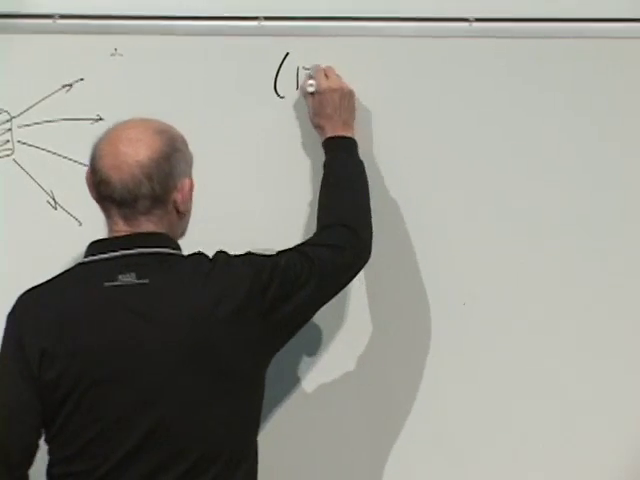
\includegraphics[width=0.66\textwidth]{lecture_06_figure_02.png}
  \caption{本講採用的度規慣例下，質量殼條件為何。}
  \lectureframe{00:05:56}
  \label{fig:l06-mass-shell}
\end{figure}

考慮兩個粒子以動量 \(k_1,k_2\) 入射，另有兩個粒子以物理動量 \(q_3,q_4\) 出射。能量與動量守恆可寫成一個四向量方程：
\begin{equation}
  k_1+k_2=q_3+q_4.
  \label{eq:l06-physical-conservation}
\end{equation}
方便的作法是把每條外線的動量都定義為入射動量：
\begin{equation}
  k_3\equiv-q_3,
  \qquad
  k_4\equiv-q_4.
\end{equation}
如此一來
\begin{equation}
  k_1+k_2+k_3+k_4=0,
  \label{eq:l06-all-incoming}
\end{equation}
而且每條外腿都滿足 \(k_i^2=-m_i^2\)。出射粒子只有在這套記帳慣例下才具有負能量；它們的物理能量仍為正。

\begin{figure}[H]
  \centering
  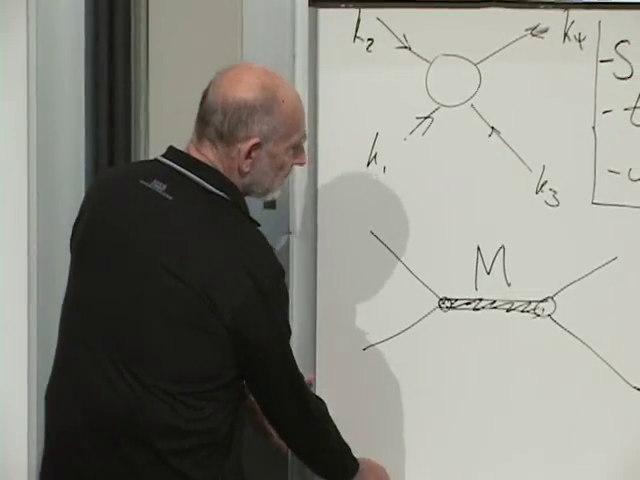
\includegraphics[width=0.68\textwidth]{lecture_06_figure_03.png}
  \caption{將物理出射動量反向，便可對稱地把四個外部動量全都視為入射。}
  \lectureframe{00:09:10}
  \label{fig:l06-all-incoming-board}
\end{figure}

乍看之下，振幅是十六個分量的函數，
\(\mathcal A(k_1,k_2,k_3,k_4)\)。其中大多數都是多餘的。轉到質心參考系，將入射動量旋轉至選定的軸上，並為求簡便，假設四個粒子的質量相同。如此一來，入射態便由一個數值決定，也就是質心能量。出射粒子的空間動量大小相等、方向相反，且大小與入射粒子對相同。剩下的只有偏轉角 \(\theta\)。因此，這個過程有兩個獨立的運動學變數：
\begin{equation}
  E_{\mathrm{cm}},
  \qquad
  \theta.
  \label{eq:l06-two-data}
\end{equation}

\section{Mandelstam 變數}

\eqref{eq:l06-two-data} 中的兩個物理量應能不依賴參考系地表示。採用全入射慣例，定義
\begin{equation}
  \begin{aligned}
    -s&=(k_1+k_2)^2,\\
    -t&=(k_1+k_3)^2,\\
    -u&=(k_1+k_4)^2.
  \end{aligned}
  \label{eq:l06-mandelstam}
\end{equation}
在質心參考系中，\(k_1+k_2\) 的空間部分彼此抵消，因此
\begin{equation}
  s=E_{\mathrm{cm}}^2.
  \label{eq:l06-s-energy}
\end{equation}

對出射粒子的物理動量 \(q_3=-k_3\)，
\begin{equation}
  k_1+k_3=k_1-q_3
\end{equation}
是由外腿 1 傳遞至外腿 3 的動量。若外部粒子的質量相同，且入射空間動量的大小為 \(p\)，則
\begin{equation}
  -t=2p^2(1-\cos\theta),
  \qquad
  -u=2p^2(1+\cos\theta).
  \label{eq:l06-tu-angle}
\end{equation}
因此，\(t\) 和 \(u\) 承載著探測器所測得的角度資訊。

\begin{figure}[H]
  \centering
  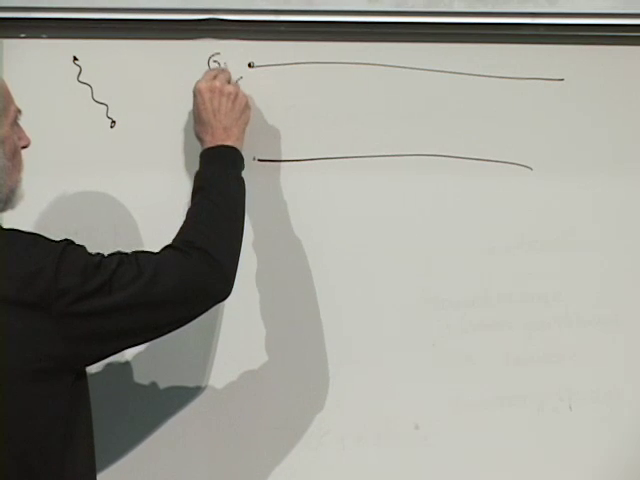
\includegraphics[width=0.74\textwidth]{lecture_06_figure_04.png}
  \caption{全入射慣例下 \(s,t,u\) 的對稱定義。}
  \lectureframe{00:26:20}
  \label{fig:l06-stu-board}
\end{figure}

三個符號不代表有三項獨立資料。將 \eqref{eq:l06-all-incoming} 平方並利用 \(k_i^2=-m^2\)，對等質量情況可得
\begin{equation}
  s+t+u=4m^2
  \label{eq:l06-stu-constraint}
\end{equation}
已知 \(s\) 與 \(t\) 後，\(u\) 便隨之確定。

\begin{classroomqa}
\audiencequestion{真空會像摩擦力一樣，使自由運動的粒子減速嗎？\lecturetimestamp{00:27:17}}
\lecturerresponse{在平移不變的真空中不會。動量不可能憑空消失，因此動量守恆禁止這種摩擦。可以設想某種介質，或另一種選定了優先靜止參考系的真空，但這裡討論的並非那種真空。}
\end{classroomqa}

\begin{classroomqa}
\audiencequestion{為什麼兩個出射粒子的能量必須相同？\lecturetimestamp{00:27:54}}
\lecturerresponse{在質心參考系中，兩者的空間動量必須大小相等、方向相反。對於這裡討論的等質量過程，動量大小相等，再由 \(E^2=p^2+m^2\) 可知能量也相等。若出射粒子的質量不同，這個結論就必須修正。}
\end{classroomqa}

\section{直接道與交叉道}

在一個簡單的點粒子圖中，粒子 1 和 2 形成質量為 \(M\) 的中間粒子，接著衰變成 3 和 4。略去分子因子及極點處方後，其典型依賴形式為
\begin{equation}
  \mathcal A_s\sim\frac{g^2}{s-M^2}.
  \label{eq:l06-s-channel}
\end{equation}
這是直接過程，也就是 \(s\) 道過程。將連結方式轉向一側，便得到兩條外線之間的交換：
\begin{equation}
  \mathcal A_t\sim\frac{g^2}{t-M^2},
  \label{eq:l06-t-channel}
\end{equation}
這是交叉過程，也就是 \(t\) 道過程。第三種連結方式則給出
\begin{equation}
  \mathcal A_u\sim\frac{g^2}{u-M^2}.
  \label{eq:l06-u-channel}
\end{equation}

\begin{figure}[H]
  \centering
  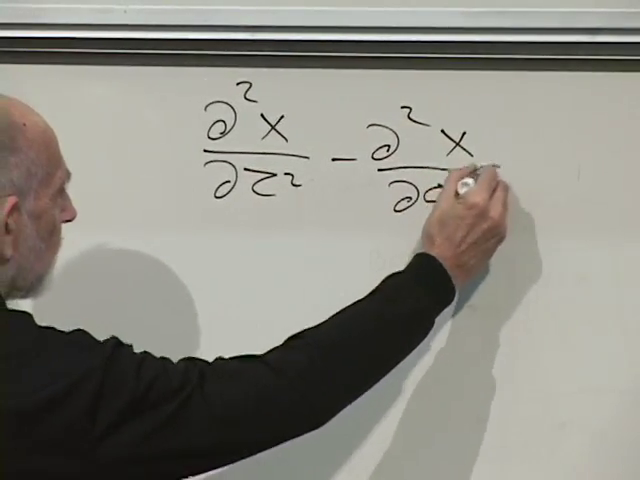
\includegraphics[width=0.72\textwidth]{lecture_06_figure_05.png}
  \caption{經由中間態直接生成，以及相應的極點 \(g^2/(s-M^2)\)；同一塊板上也正在拼出交叉道的連結方式。}
  \lectureframe{00:30:50}
  \label{fig:l06-channel-board}
\end{figure}

這項區別具有物理意義。在這個粗略的純量近似下，\eqref{eq:l06-s-channel} 取決於碰撞能量，而不取決於角度。複合態在衰變前已不再保留入射方向的資訊，因此衰變是各向同性的。交換振幅則取決於動量轉移，因而也取決於角度；交換粒子越輕，越傾向於小角度偏轉。自旋還會帶來額外的角度依賴，但極點結構在此已清楚可見。

\begin{classroomqa}
\audiencequestion{缺少的 \(u\) 道會不會產生第三項？\lecturetimestamp{00:34:47}}
\lecturerresponse{會，只要粒子的種類與耦合允許這種連結方式，就要加入在 \(u=M^2\) 有極點的一項。它不是新的獨立運動學變數，因為 \(s+t+u=4m^2\)；不過，它確實對應一種不同的道圖。}
\end{classroomqa}

\section{一個函數，兩種通道描述}

單一極點不足以描述介子散射。兩個介子可以形成許多共振態，具有一系列不同的質量與角動量。1960 年代初期，人們的第一個想法是加入更多 \(s\) 道極點、更多 \(t\) 道極點，以及所有允許的 \(u\) 道極點。後來，人們找到了一個精簡得多的函數。在本講採用的單位制中，線性 Regge 軌跡及其截距已吸收到 \(s\) 與 \(t\) 中，振幅為
\begin{equation}
  \mathcal A_{\mathrm V}(s,t)
  \propto
  \frac{\Gamma(-s)\Gamma(-t)}{\Gamma(-s-t)}.
  \label{eq:l06-veneziano}
\end{equation}
伽馬函數將階乘延伸為
\begin{equation}
  \Gamma(n)=(n-1)!
\end{equation}
此式在正整數處成立。

\begin{figure}[H]
  \centering
  \includegraphics[width=0.68\textwidth]{lecture_06_figure_06.png}
  \caption{以伽馬函數的對稱比值表示的 Veneziano 振幅。}
  \lectureframe{00:42:25}
  \label{fig:l06-veneziano-board}
\end{figure}

\(\Gamma(-s)\) 的極點重現了直接道共振態的無限序列。然而，同一個表示式在 \(s\leftrightarrow
t\) 下保持對稱，因此 \(\Gamma(-t)\) 的極點可展開成交叉道描述。這並非把兩項分別加入振幅；一個解析函數便容許兩種描述。這就是直接道共振態與交叉道交換之間的對偶性。

\begin{classroomqa}
\audiencequestion{一個振幅怎麼能同時包含兩個通道的求和，卻不把它們相加？\lecturetimestamp{00:43:32}}
\lecturerresponse{這正是令人驚訝之處。在 \(s\) 道極點附近展開這個函數，會得到直接道共振態的組織方式；在 \(t\) 道極點附近展開，則會以交換的方式呈現同一個函數。要說明這兩種解讀為何相同，必須有微觀模型，而這個模型就是相互作用的弦。}
\end{classroomqa}

\section{開弦掃出的一條帶狀面}

用下式參數化一條開弦：
\begin{equation}
  0\leq\sigma\leq\pi.
\end{equation}
標記 \(\sigma\) 並非時空位置。嵌入座標 \(X^\mu(\sigma,\tau)\) 描述這個帶標記的點在時空中的位置，而 \(\tau\) 則量度演化。點粒子掃出一條世界線；運動中的弦則掃出二維的世界面。在自由理論中，每個嵌入座標都滿足
\begin{equation}
  \frac{\partial^2X^\mu}{\partial\tau^2}
  -
  \frac{\partial^2X^\mu}{\partial\sigma^2}
  =0.
  \label{eq:l06-wave-equation}
\end{equation}

\begin{figure}[H]
  \centering
  \includegraphics[width=0.70\textwidth]{lecture_06_figure_07.png}
  \caption{描述世界面帶狀區域上各自由弦座標的波動方程。}
  \lectureframe{00:49:10}
  \label{fig:l06-wave-equation-board}
\end{figure}

建構散射過程時，最好不要太早取連續極限。將每條弦替換為 \(n\) 個以彈簧相連的質點。世界面便成為一系列密集分布、彼此鄰近的世界線，而其正規模態就是一般的諧振子。兩條入射弦鏈可以在端點處接觸；此時一根新彈簧將兩者接合，它們作為一條較長的弦鏈演化 \(\tau\)，之後彈簧斷開，兩條出射弦鏈便形成。

\begin{figure}[H]
  \centering
  \includegraphics[width=0.72\textwidth]{lecture_06_figure_08.png}
  \medskip

  \begin{tikzpicture}[x=0.85cm,y=0.70cm]
    \draw[thick] (0,2.2) -- (2.1,2.2) -- (3.1,1.5);
    \draw[thick] (0,0.8) -- (2.1,0.8) -- (3.1,1.5);
    \draw[thick] (3.1,1.5) -- (5.5,1.5);
    \draw[thick] (5.5,1.5) -- (6.5,2.2) -- (8.6,2.2);
    \draw[thick] (5.5,1.5) -- (6.5,0.8) -- (8.6,0.8);
    \draw[<->] (3.1,0.35) -- node[below] {\(\tau\)} (5.5,0.35);
    \node[left] at (0,2.2) {1};
    \node[left] at (0,0.8) {2};
    \node[right] at (8.6,2.2) {3};
    \node[right] at (8.6,0.8) {4};
  \end{tikzpicture}
  \caption{兩條離散化的開弦相接，形成一條中間弦，持續 \(\tau\)，然後分裂。來源畫面保留了彈簧與世界線的構造；示意圖則凸顯其連結方式。}
  \lectureframe{00:51:25}
  \label{fig:l06-string-joining}
\end{figure}

圖中兩條弦只是在參數空間裡彼此相鄰。在端點座標實際重合之前，它們在時空中的位置不必相鄰。重參數化自由度讓我們可以把接合與分裂事件安排在圖中方便的位置；這項幾何自由度將在下一講轉化為共形對稱性。

\section{振子計算逐步拆解}

設第一條弦鏈的座標為 \(x_1,\ldots,x_n\)，第二條為 \(x_{n+1},\ldots,x_{2n}\)。它們的質心座標是
\begin{equation}
  X_{\mathrm{cm}}^{(1)}
  =\frac1n\sum_{a=1}^{n}x_a,
  \qquad
  X_{\mathrm{cm}}^{(2)}
  =\frac1n\sum_{a=n+1}^{2n}x_a.
  \label{eq:l06-chain-centers}
\end{equation}
動量確定為 \(k_1\) 的弦鏈，其波函數由質心平面波乘上內部振子的基態波函數構成：
\begin{align}
  \Psi_1
  &=
  e^{ik_1\cdot X_{\mathrm{cm}}^{(1)}}
  \psi_0(x_1,\ldots,x_n),
  \\
  \Psi_2
  &=
  e^{ik_2\cdot X_{\mathrm{cm}}^{(2)}}
  \psi_0(x_{n+1},\ldots,x_{2n}).
  \label{eq:l06-two-wavefunctions}
\end{align}
因子 \(\psi_0\) 只依賴相對座標，不受整條弦鏈共同平移影響。由於兩條入射弦起初是彼此分離的量子系統，
\begin{equation}
  \Psi_{\mathrm{in}}=\Psi_1\Psi_2.
  \label{eq:l06-product-state}
\end{equation}

\begin{figure}[H]
  \centering
  \includegraphics[width=0.76\textwidth]{lecture_06_figure_09.png}
  \caption{兩個動量平面波及各自的內部振子基態因子，以不同顏色表示。}
  \lectureframe{00:58:05}
  \label{fig:l06-wavefunctions-board}
\end{figure}

接合時，從這個波函數中選出兩個端點座標相等的部分：
\begin{equation}
  x_n=x_{n+1}.
  \label{eq:l06-endpoint-contact}
\end{equation}
此刻其餘座標保持不變。接著，所選出的態以單一較長弦鏈的哈密頓量 \(H_{\mathrm{joined}}\) 演化：
\begin{equation}
  \Psi(\tau)
  =
  e^{-iH_{\mathrm{joined}}\tau}\Psi(0).
  \label{eq:l06-time-evolution}
\end{equation}
最後，計算它與出射弦態乘積的重疊；這些出射態所帶的動量為 \(q_3,q_4\)。

\begin{figure}[H]
  \centering
  \includegraphics[width=0.76\textwidth]{lecture_06_figure_10.png}
  \caption{施加端點重合條件前的雙弦波函數。}
  \lectureframe{00:58:55}
  \label{fig:l06-endpoint-board}
\end{figure}

計算過程冗長，但並不神祕。每個內部座標都能分解為振子模態，因此接合時的重疊、時間演化與最後的投影，都可化為高斯振子的代數計算。尚未確定的只有接合後弦的存續時間 \(\tau\)。

\begin{classroomqa}
\audiencequestion{黑色和紅色的波函數要相加還是相乘？\lecturetimestamp{01:02:26}}
\lecturerresponse{相乘。兩個獨立系統的張量積態，在座標表象中以各自波函數的乘積表示。相加描述的是不同可能性間的疊加，而不是兩條入射弦同時存在。}
\end{classroomqa}

\begin{classroomqa}
\audiencequestion{為什麼要對中間時間 \(\tau\) 積分？\lecturetimestamp{01:04:04}}
\lecturerresponse{接合後的弦沒有固定的存續時間。依照費曼規則，必須對所有允許的歷史求振幅和。在這種描述中，剩下的連續歷史參數就是從接合到分裂之間的時間，因此求和便化為對 \(0\leq\tau<\infty\) 的積分。}
\end{classroomqa}

\section{從傳播時間到貝塔函數}

計算完振子重疊後，結果可整理為
\begin{equation}
  \mathcal A(s,t)
  \propto
  \int_0^\infty d\tau\,
  e^{\tau(s+1)}
  \bigl(1-e^{-\tau}\bigr)^{-t-1}
  e^{-\tau}.
  \label{eq:l06-tau-integral}
\end{equation}
最後的 \(e^{-\tau}\) 保留在式中，因為下一步的變數代換需要它作為雅可比因子。等價地，首尾兩個指數因子可合併為 \(e^{s\tau}\)。

\begin{figure}[H]
  \centering
  \includegraphics[width=0.76\textwidth]{lecture_06_figure_11.png}
  \caption{振子計算後的傳播時間積分式；獨立的 \(e^{-\tau}\) 因子提供變數代換所需的雅可比因子。}
  \lectureframe{01:06:45}
  \label{fig:l06-tau-integral-board}
\end{figure}

現在令
\begin{equation}
  z=e^{-\tau},
  \qquad
  dz=-e^{-\tau}\,d\tau.
  \label{eq:l06-z-substitution}
\end{equation}
當 \(\tau\) 從 \(0\) 增至 \(\infty\) 時，\(z\) 會從 \(1\) 降至 \(0\)。負號使積分上下限反轉，因此得到
\begin{equation}
  \mathcal A(s,t)
  \propto
  \int_0^1
  z^{-s-1}(1-z)^{-t-1}\,dz.
  \label{eq:l06-beta-integral}
\end{equation}

\begin{figure}[H]
  \centering
  \includegraphics[width=0.74\textwidth]{lecture_06_figure_12.png}
  \caption{代換 \(z=e^{-\tau}\) 顯示出尤拉貝塔積分的形式。}
  \lectureframe{01:08:49}
  \label{fig:l06-beta-integral-board}
\end{figure}

在端點收斂的範圍內，這個積分有直接定義；在其他範圍則以解析延拓定義。它就是尤拉貝塔函數：
\begin{equation}
  B(-s,-t)
  =
  \frac{\Gamma(-s)\Gamma(-t)}{\Gamma(-s-t)}.
  \label{eq:l06-beta-gamma}
\end{equation}

\begin{figure}[H]
  \centering
  \includegraphics[width=0.72\textwidth]{lecture_06_figure_13.png}
  \caption{黑板將變換後的積分辨認為 \(B(-s,-t)\)，並開始還原其伽馬函數形式。}
  \lectureframe{01:12:24}
  \label{fig:l06-beta-gamma-board}
\end{figure}

通道對稱性現在一目了然。在 \(z\mapsto1-z\) 下，
\begin{equation}
  \int_0^1 z^{-s-1}(1-z)^{-t-1}\,dz
  =
  \int_0^1 z^{-t-1}(1-z)^{-s-1}\,dz.
\end{equation}
因此 \(\mathcal A(s,t)=\mathcal A(t,s)\)。由兩條弦接合、之後再分裂所建構的過程，自然也包含交叉道的描述。
\editorialnote{本講在貝塔函數的引數中省略了 Regge 斜率與截距。標準記號會將 \(s,t\) 替換為相應的線性軌跡 \(\alpha(s),\alpha(t)\)。對偶性與變數代換的論證不受影響。}

\begin{classroomqa}
\audiencequestion{伽馬函數比值看起來像組合學中的階乘式。它是否有直接的物理計數詮釋？\lecturetimestamp{01:13:22}}
\lecturerresponse{在整數引數下，貝塔函數與例如 \(n!\,m!/(n+m)!\) 這樣的比值有關，但這裡並未主張存在某種組合機制。世界面積分也恰好會產生同一個特殊函數；不過，發現這個振幅的過程並非從這種類比出發。}
\end{classroomqa}

一個世界面之所以能以兩種通道來解讀，其背後尚未揭示的原因是共形對稱性。它允許像拉伸太妃糖一樣延展這個面，而不改變振幅，因而能將直接道中長時間的傳播區域轉換成交叉道的交換圖像。這項幾何解釋留待下一講討論。

\section{散射檢驗確立了什麼}
\enlargethispage{3\baselineskip}
\begingroup
\setlength{\medskipamount}{3pt plus 1pt minus 1pt}

離散弦鏈的接合圖像引出了最後一組問題。

\begin{classroomqa}
\audiencequestion{若兩條各由 \(n\) 個組成部分構成的弦鏈在端點接合，接合後是否會有 \(2n-1\) 個組成部分？這會改變費米子宇稱嗎？\lecturetimestamp{01:16:16}}
\lecturerresponse{在強子端點圖像中，相接觸的端點對可視為一對粒子與反粒子，兩者湮滅後，數目減少二，而非一。在連續極限下，\(2n\) 與 \(2n-2\) 之間的有限差異無關緊要；但費米子宇稱必須保持不變。格點上的組成部分只是連續弦的調節器，並非字面意義上的基本珠粒。}
\end{classroomqa}

\begin{classroomqa}
\audiencequestion{後續討論會深入介紹超弦的完整數學嗎？\lecturetimestamp{01:18:05}}
\lecturerresponse{只會用到其中選定的推論。接下來將討論世界面對稱性與緊緻化，之後再從另一個出發點切入：這個出發點於 1990 年代中期發展而成，也就是 M 理論。它的目標是從另一種觀點得到相同的物理；在這種觀點下，若干原本複雜的特徵會變得清晰。}
\end{classroomqa}

\begin{classroomqa}
\audiencequestion{這項接合規則只是從介子碰撞得到的線索嗎？\lecturetimestamp{01:20:02}}
\lecturerresponse{介子散射提供了歷史上的線索，但這項規則普遍適用於開弦。同樣的拓撲也描述開弦光子與其他開弦態的碰撞。兩條閉弦也會以類似方式接合與分裂，中間區域則是一條閉弦。}
\end{classroomqa}

\begin{classroomqa}
\audiencequestion{這項計算只適用於弦態為費米子的情況嗎？\lecturetimestamp{01:20:56}}
\lecturerresponse{不適用。最初的 Veneziano 計算描述的是玻色開弦。超弦需要額外的費米自由度，且被積函數的細節也會有所改變，但接合、傳播、投影與世界面對偶性的邏輯仍大致相同。}
\end{classroomqa}

在振子譜中找到自旋一或自旋二的態，固然令人振奮，卻還不足以證明其身分。它們的散射振幅提供了更有力的檢驗。光子振幅符合電荷守恆與規範不變性所要求的恆等式；引力子振幅則符合無質量自旋二場的相應限制。弦態在與有質量態及無質量態的交互作用中，以及彼此交互作用時，都通過了這些檢驗。因此，光子與引力子的稱呼是基於物理上的確認，而非僅憑極化態計數猜測。
\editorialnote{以現代術語來說，這些檢驗體現於非物理極化態的解耦、規範 Ward 恆等式，以及無質量自旋二態的普適低能耦合。}

\begin{classroomqa}
\audiencequestion{弦理論描述中的電荷本身從何而來？\lecturetimestamp{01:24:03}}
\lecturerresponse{講座結尾時，這個問題仍未解答。要回答它，必須先介紹弦理論的內部結構與端點結構；這些內容尚未談到，因此答案留待後續討論，而不屬於此處的散射推導。}
\end{classroomqa}
\endgroup

\chapter{世界面、威克轉動與道對偶}

\lectureoverview{粒子沿著世界線運動；弦則掃出一個世界面。將任一物體量子化，都需要對所有可能的歷史求和，但洛侖茲時空中的求和帶有振盪相位，難以定義。將世界面時間轉為虛座標後，便得到由拉普拉斯方程支配的歐幾里得理論。其共形對稱性接著可將四弦交互作用的帶縫曲面映成帶有四個邊界插入點的圓盤，讓直接道與交叉道之間的對稱性顯現出來。}

\section{從世界線到對所有歷史求和}

先從一個自由粒子談起。在非相對論力學中，粒子的位置是函數\(\mathbf x(t)\)；將質量設為 1 後，其作用量為
\begin{equation}
  S_{\mathrm{NR}}[\mathbf x]
  =\frac12\int_{t_1}^{t_2}\dot{\mathbf x}^{\,2}\,dt.
  \label{eq:l07-nr-action}
\end{equation}
對相對論性描述而言，更自然的做法是將時間和空間納入同一個向量\(X^\mu(\tau)\)，並以\(\tau\)作為沿軌跡的參數。相應的二次形式為
\begin{equation}
  S_{\mathrm{rel}}[X]
  =\frac12\int_{\tau_1}^{\tau_2}
  \frac{dX^\mu}{d\tau}\frac{dX_\mu}{d\tau}\,d\tau.
  \label{eq:l07-rel-action}
\end{equation}
上下指標反映了時間與空間之間的洛侖茲號差。
\editorialnote{此處使用的是固定世界線參數化下的二次相對論作用量。另一種明確具有重參數化不變性的形式，則正比於固有長度；講座稍後會提到這一點。}

\begin{figure}[H]
  \centering
  \includegraphics[width=0.72\textwidth]{lecture_07_figure_01.png}
  \caption{黑板上並列寫出非相對論作用量及其相對論二次形式。}
  \lectureframe{00:03:35}
  \label{fig:l07-particle-actions}
\end{figure}

在經典力學中，固定端點後對路徑作變分。自由粒子便沿著速度恆定的直線世界線運動。量子力學問的則是另一個問題：它不會在兩個端點之間選出一條軌跡，而是要問粒子從一點出發、並在另一點被探測到的振幅。每一條中間路徑都會貢獻一個相位，
\begin{equation}
  K(2,1)=\int_{X(1)}^{X(2)}\!\mathcal D X\,
  e^{iS[X]}.
  \label{eq:l07-feynman-integral}
\end{equation}
泛函積分是對無限維路徑空間所作的積分，並非作用量中已出現的普通積分。

\begin{figure}[H]
  \centering
  \includegraphics[width=0.72\textwidth]{lecture_07_figure_02.png}
  \caption{對所有軌跡求和之前，一條代表性路徑及其所帶的相位。}
  \lectureframe{00:06:21}
  \label{fig:l07-path-integral-board}
\end{figure}

用相對論的語言來說，這個點到點的振幅就是傳播子。在交互作用中，數段世界線會在某處相接。將各段的作用量相加，對相接點積分，再對符合外部粒子要求的圖形求和。因此，熟悉的費曼圖展開，其實已隱含在對所有歷史求和的指示之中。

此處以符號\(S\)表示作用量。它與熵無關，也與講座接近尾聲時使用的曼德斯塔姆變數\(s\)無關。兩者沿用相同記號只是傳統如此，並沒有特別的啟發性。

\section{將時間轉向側面}

\eqref{eq:l07-feynman-integral}有個立即浮現的問題。每個因子\(e^{iS}\)的絕對值都是 1。因此，劇烈振盪的軌跡和經典直線的絕對權重相同，兩者只有相位不同。相消干涉會讓經典行為重新顯現，但不會因此使形式上的積分成為普通的收斂積分。

引入新的參數\(s\)，令
\begin{equation}
  \tau=\alpha s,
  \qquad
  d\tau=\alpha\,ds,
  \qquad
  \frac{dX}{d\tau}=\frac{1}{\alpha}\frac{dX}{ds}.
\end{equation}
如此一來，二次作用量會按下式重新縮放：
\begin{equation}
  \frac12\int d\tau
  \left(\frac{dX}{d\tau}\right)^2
  =
  \frac{1}{2\alpha}\int ds
  \left(\frac{dX}{ds}\right)^2.
  \label{eq:l07-rescaled-action}
\end{equation}
選取對應於\(\alpha=-i\)的積分路徑後，振盪權重便轉為
\begin{equation}
  e^{iS}
  \longrightarrow
  \exp\!\left[-\frac12\int ds
  \left(\frac{dX}{ds}\right)^2\right]
  =e^{-S_E}.
  \label{eq:l07-euclidean-particle}
\end{equation}

\begin{figure}[H]
  \centering
  \includegraphics[width=0.66\textwidth]{lecture_07_figure_03.png}
  \caption{代入虛時間後的歐幾里得粒子權重；指數為實數且不大於零。}
  \lectureframe{00:16:20}
  \label{fig:l07-particle-wick}
\end{figure}

跑到很遠再折返，或是沒有走遠卻快速來回擺動的路徑，都會有很大的正\(S_E\)，因而受到指數抑制。所得的是一種維納型積分，已有嚴謹的收斂理論。從實數\(\tau\)延伸而來的端點，位於虛數\(s\)的積分路徑上。實際計算時，先在收斂區域內求出歐幾里得量，再將答案解析延拓回物理的洛侖茲變數。這個操作就是威克轉動：計算時將時間轉向側面，而非將時間捨去。

\section{從世界線到世界面}

點粒子有一條世界線。開弦掃出一條帶狀曲面，閉弦則掃出一個管狀曲面。座標\((\sigma,\tau)\)標記二維世界面上的各點，而
\begin{equation}
  X^\mu=X^\mu(\sigma,\tau)
  \label{eq:l07-embedding}
\end{equation}
則給出各標記點在時空中的位置。知道所有函數\(X^\mu\)，就完整指定了弦的歷史。

洛侖茲世界面上的二次作用量，具有與普通振動弦相同的動能減位能結構：
\begin{equation}
  S_{\mathrm{ws}}[X]
  =\frac{T_s}{2}\int d\tau\,d\sigma\,
  \left[
    \partial_\tau X^\mu\partial_\tau X_\mu
    -
    \partial_\sigma X^\mu\partial_\sigma X_\mu
  \right].
  \label{eq:l07-lorentzian-worldsheet}
\end{equation}
整體張力\(T_s\)決定尺度；本講聚焦於導數結構，因此暫且省略這個因子。

\begin{figure}[H]
  \centering
  \includegraphics[width=0.72\textwidth]{lecture_07_figure_04.png}
  \caption{\(X^\mu(\sigma,\tau)\)的洛侖茲世界面作用量，其符號呈現動能減位能的結構。}
  \lectureframe{00:24:26}
  \label{fig:l07-worldsheet-action}
\end{figure}

弦的振幅是將此作用量指數化，並對所有連接指定初態與末態弦構形的曲面求和而得：
\begin{equation}
  \mathcal A=\int\mathcal D X\,e^{iS_{\mathrm{ws}}[X]}.
  \label{eq:l07-surface-integral}
\end{equation}
同一條規則適用於兩條弦變成兩條、兩條弦變成三條，或任何其他允許的外部構形。求和也包含不同拓撲的世界面。在點粒子圖形展開中增加圈圖階數，對應到弦理論中增加洞。

\begin{figure}[H]
  \centering
  \includegraphics[width=0.66\textwidth]{lecture_07_figure_05.png}
  \caption{連接數條外部弦的曲面；其中一個洞代表不同拓撲的世界面。}
  \lectureframe{00:27:14}
  \label{fig:l07-surface-topology}
\end{figure}

\begin{classroomqa}
\audiencequestion{對點電子而言，\(\sigma\)導數會直接消失嗎？\lecturetimestamp{00:27:56}}
\lecturerresponse{點粒子一開始就沒有\(\sigma\)座標。不過，這些圖像彼此相關：當外部態的能量相較於弦尺度很低，且過程能量也很低時，弦振幅會重現普通的點粒子費曼圖。這個極限不只是將某個導數設為零。}
\end{classroomqa}

曲面積分和路徑積分有相同的收斂問題。將世界面時間作威克轉動後，穩定的歐幾里得形式為
\begin{equation}
  \begin{aligned}
    S_{E,\mathrm{ws}}[X]
    &=\frac{T_s}{2}\int d\tau\,d\sigma\,
      \left[
        \partial_\tau X^\mu\partial_\tau X_\mu
        +\partial_\sigma X^\mu\partial_\sigma X_\mu
      \right],\\
    \mathcal A_E&=\int\mathcal D X\,e^{-S_{E,\mathrm{ws}}}.
  \end{aligned}
  \label{eq:l07-euclidean-worldsheet}
\end{equation}
現在兩個導數項都帶有相同的正號。劇烈振動或大幅延展的曲面具有很大的歐幾里得作用量，因此受到抑制。

\begin{figure}[H]
  \centering
  \includegraphics[width=0.72\textwidth]{lecture_07_figure_06.png}
  \caption{將\(\tau\)轉為虛時間後，歐幾里得世界面密度中的各項皆為正。}
  \lectureframe{00:34:29}
  \label{fig:l07-worldsheet-wick}
\end{figure}

還有一種幾何上更直接的表述方式。可以為相對論粒子指定一個正比於其路徑固有長度的作用量；也可以為弦指定一個正比於其世界面時空面積的作用量。後者稱為南部--後藤作用量。此處使用的二次世界面形式，慣稱波利亞科夫形式，對目前的計算而言容易得多。
\editorialnote{講座以幽默方式談到歷史上的命名，也提及相關的劉維爾作用量和狄利克雷邊界條件。此處的推導不涉及優先權主張，只用到面積形式與輔助度規形式的等價性。}

\section{歐幾里得運動方程}

座標\(\sigma\)和\(\tau\)只是世界面上的標記。接下來自然要問：哪些重新標記不會改變理論？從運動方程最容易看出答案。對\eqref{eq:l07-euclidean-worldsheet}作變分，逐分量可得
\begin{equation}
  \partial_\tau^2X^\mu+\partial_\sigma^2X^\mu=0.
  \label{eq:l07-laplace}
\end{equation}
威克轉動之前，相對符號為負，這是波動方程。在歐幾里得號誌下，兩個符號都為正，因此得到二維拉普拉斯方程。

\begin{classroomqa}
\audiencequestion{這是振動鼓面的方程嗎？
\lecturetimestamp{00:41:50}}
\lecturerresponse{它和振動鼓面的方程密切相關，但鼓面振動還包含一個實數時間座標，因此服從波動方程。此處的方程是歐幾里得拉普拉斯方程。無電荷區域中的靜電位，是更直接而熟悉的例子。}
\end{classroomqa}

\begin{classroomqa}
\audiencequestion{作用量含有一階導數，為什麼運動方程卻含有二階導數？\lecturetimestamp{00:42:44}}
\lecturerresponse{對一階導數的二次項作變分，再分部積分，會將一個導數移到該一階導數上。這是場論中的對應情形：作用量裡的\(\dot x^{\,2}\)會在運動方程中產生\(\ddot x\)。}
\end{classroomqa}

\begin{figure}[H]
  \centering
  \includegraphics[width=0.68\textwidth]{lecture_07_figure_07.png}
  \caption{帶正號的拉普拉斯方程，以及用來解讀其二階導數的第一個離散式。}
  \lectureframe{00:43:30}
  \label{fig:l07-laplace-board}
\end{figure}

為了看清其中的幾何，先以間距\(\epsilon\)離散化一個座標。一階導數是相鄰點之差；二階導數則是相鄰差分之差：
\begin{equation}
  \frac{d^2X}{ds^2}\bigg|_{2}
  \longrightarrow
  \frac{X(3)-2X(2)+X(1)}{\epsilon^2}.
  \label{eq:l07-second-difference}
\end{equation}

\begin{figure}[H]
  \centering
  \includegraphics[width=0.72\textwidth]{lecture_07_figure_08.png}
  \caption{編號的直線、小格點區域，以及二階導數的有限差分展開式。}
  \lectureframe{00:45:51}
  \label{fig:l07-finite-difference-board}
\end{figure}

現在將\((\sigma,\tau)\)平面離散化。將中心點\(5\)的四個最近鄰標記為\(1,2,3,4\)。方程\eqref{eq:l07-laplace}變成
\begin{equation}
  X(1)+X(2)+X(3)+X(4)-4X(5)=0,
\end{equation}
也就是
\begin{equation}
  X(5)=\frac14\bigl[X(1)+X(2)+X(3)+X(4)\bigr].
  \label{eq:l07-mean-value}
\end{equation}

\begin{figure}[H]
  \centering
  \includegraphics[width=0.72\textwidth]{lecture_07_figure_09.png}
  \caption{完整的二維有限差分方程：中心點的值等於四個鄰點的平均值。}
  \lectureframe{00:48:26}
  \label{fig:l07-mean-value-board}
\end{figure}

這個平均值性質對任意取向的無窮小正方形都成立。它呈現了拉普拉斯方程的局部幾何意涵，也是通往共形對稱性的橋梁。

\section{共形座標}

考慮從\((\sigma,\tau)\)到\((\sigma',\tau')\)的變換。一般形變會將小正方形變成任意四邊形。此處關注的特殊變換，則會將每個無窮小正方形映成另一個無窮小正方形，並可能使它旋轉或縮放。換句話說，這些變換會保留曲線相交時的角度，稱為共形變換。

\begin{figure}[H]
  \centering
  \includegraphics[width=0.68\textwidth]{lecture_07_figure_10.png}
  \caption{局部正方形映成另一個小圖形，同時檢視角度是否保持不變。}
  \lectureframe{00:53:25}
  \label{fig:l07-conformal-board}
\end{figure}

\begin{classroomqa}
\audiencequestion{如果角度保持不變，這種變換基本上就只是旋轉嗎？\lecturetimestamp{00:53:31}}
\lecturerresponse{只在局部如此；即使在局部，還可以有一致的尺度變化。局部旋轉角度與尺度因子可以隨位置改變，因此座標網格可以彎曲、在某個區域放大，並在另一個區域縮小，同時保持無窮小的形狀。}
\end{classroomqa}

保角映射不一定保持大小。如果大小也處處固定，可能的變換就會縮減為範圍小得多的剛體變換，也就是平移和旋轉。共形映射則保留局部形狀。這就是為什麼地圖投影能保持小島的形狀，卻大幅扭曲其面積。

\begin{classroomqa}
\audiencequestion{共形映射是否等同於座標系是平坦的？\lecturetimestamp{00:55:35}}
\lecturerresponse{不是。平坦性和共形性是不同的概念。共形映射可以採用彎曲的座標線；它保留的是相交曲線之間的角度。墨卡托式地圖投影是熟悉的例子：它保留局部形狀，卻造成顯著的尺度失真。}
\end{classroomqa}

在二維中，所需的變換在局部由複數座標\begin{equation}
  z=\sigma+i\tau.
\end{equation}的解析函數生成。
有限邊界經映射後，外觀可能大幅改變。正方形區域可以映成平滑區域，原來的角會映到新邊界上的一般位置，而非視覺上突出的點。這並不矛盾：共形性是局部的內部條件，只要映射在某處正則，就會在該處保留無窮小角度。

\begin{classroomqa}
\audiencequestion{這種座標自由度，是否就是先前的接合--分裂圖可以採用對稱形式的原因？
\lecturetimestamp{00:56:32}}
\lecturerresponse{是。保留世界面方程的共形自由度，使我們能將形狀不規則的交互作用帶映成較對稱的區域。剩餘的自由度並未消除物理上的接合--分裂參數，而是將它改以邊界插入點的相對位置來表示。}
\end{classroomqa}

\section{帶縫曲面與圓盤}

回到四弦散射。兩條開弦進入，端點接合，合併後的弦傳播一段時間，之後再分裂。若將這個過程畫成平坦的世界面，它就是一條兩端各有一道縫的無限長帶。兩道縫尖端之間的距離\(\tau_0\)代表中間弦的存續時間，振幅須對這段時間積分。

\begin{figure}[H]
  \centering
  \includegraphics[width=0.72\textwidth]{lecture_07_figure_11.png}
  \caption{雙縫長帶表示兩條開弦接合、合併傳播，之後再度分裂。}
  \lectureframe{01:00:20}
  \label{fig:l07-slit-strip}
\end{figure}

歐幾里得化後，這個區域上的嵌入場滿足拉普拉斯方程。因此，共形不變性允許將帶縫長帶映成圓盤。要看出兩者的拓撲關係，可以先用同心圓將圓盤分層，再連續形變這些閉合曲線，直到它們填滿帶縫區域。映射會將無窮遠處的端點變成特殊的邊界點。

\begin{figure}[H]
  \centering
  \includegraphics[width=0.72\textwidth]{lecture_07_figure_12.png}
  \medskip

  \begin{adjustbox}{max width=\linewidth}
  \begin{tikzpicture}[x=0.75cm,y=0.75cm]
    \draw[thick] (-5,1.2) -- (-1.2,1.2) -- (-0.35,0.35);
    \draw[thick] (-5,-1.2) -- (-1.2,-1.2) -- (-0.35,-0.35);
    \draw[thick] (0.35,0.35) -- (1.2,1.2) -- (5,1.2);
    \draw[thick] (0.35,-0.35) -- (1.2,-1.2) -- (5,-1.2);
    \draw[->,thick] (5.6,0) -- (7.0,0);
    \draw[thick] (9.0,0) circle (1.45);
    \foreach \a in {40,140,220,320} \fill (9.0,0) ++(\a:1.45) circle (1.5pt);
    \node[below] at (0,-1.65) {slit strip};
    \node[below] at (9.0,-1.65) {disc};
  \end{tikzpicture}
  \end{adjustbox}
  \caption{黑板上的等值線比較，以及將帶縫長帶共形映射至圓盤的清晰示意圖。四個外部端點映成四個特殊的邊界點。}
  \lectureframe{01:04:46}
  \label{fig:l07-strip-to-disc}
\end{figure}

改變座標並不會讓外部態消失。動量、粒子種類和振子能階都必須插入四個特殊點。承載這些資訊的形式物件稱為頂點算符。雖然其詳細構造留待後續討論，它們的作用已很清楚：將原本均勻的世界面路徑積分，轉化為指定的散射實驗。

利用圓盤的共形變換，將三個邊界點移至方便的參考位置後，還會剩下一個實數的相對位置。這個位置可用四個依序排列的邊界點之交比表示。它就是原先存續時間\(\tau_0\)在圓盤上的對應量。

\begin{figure}[H]
  \centering
  \includegraphics[width=0.62\textwidth]{lecture_07_figure_13.png}
  \caption{圓盤邊界上的四個插入點。共形自由度可消去其有序配置中除一個實模數外的所有模數。}
  \lectureframe{01:10:55}
  \label{fig:l07-four-points}
\end{figure}

因此，存續時間的積分並未消失，而是轉為對剩餘模數積分。採用慣用座標\(0<z<1\)時，四點開弦積分與上一講所得的形式相同：
\begin{equation}
  \mathcal A(s,t)\propto
  \int_0^1 z^{-s-1}(1-z)^{-t-1}\,dz.
  \label{eq:l07-modulus-integral}
\end{equation}

\section{同一曲面的兩種極限}

在模空間的一端，與入射粒子對應的兩個插入點彼此靠近。在帶縫長帶的座標中，這代表接合與分裂之間有一段很長的間隔：直接道中的中間弦會長時間傳播。在另一端，另一對相鄰插入點彼此靠近。此時，同一曲面自然可解讀為交叉道交換。這兩種描述在長帶圖像中看似毫不相關，卻是同一圓盤積分在相鄰邊界處的極限。

回到上一講採用的 mostly-plus 慣例，
\begin{equation}
  -s=(k_1+k_2)^2,
  \qquad
  -t=(k_1+k_3)^2.
  \label{eq:l07-mandelstam}
\end{equation}
直接道極限中的極點由\(s\)組織；交叉道極限中的極點則由\(t\)組織。
\editorialnote{講座接近尾聲時，黑板以簡寫符號表示曼德斯塔姆不變量，同時將\(s\)認定為正的質心系能量平方。方程\eqref{eq:l07-mandelstam}沿用第6講確立的 mostly-plus 慣例。}

\begin{figure}[H]
  \centering
  \includegraphics[width=0.62\textwidth]{lecture_07_figure_14.png}
  \caption{兩種道的圖示：一種取向呈現長時間傳播，交叉取向則呈現交換。}
  \lectureframe{01:19:27}
  \label{fig:l07-channel-diagrams}
\end{figure}

\begin{figure}[H]
  \centering
  \includegraphics[width=0.72\textwidth]{lecture_07_figure_15.png}
  \caption{黑板再次列出\(s\)道與\(t\)道的動量配對，並比較圓盤模數的兩個極限。}
  \lectureframe{01:19:40}
  \label{fig:l07-st-board}
\end{figure}

因此，同一個解析函數提供了兩種展開：
\begin{equation}
  \mathcal A(s,t)=\mathcal A(t,s).
\end{equation}
這就是道對偶。在最初以共振描述的脈絡中，對直接道態求和竟然也能編碼交叉道交換，曾令人覺得不可思議。在歐幾里得世界面上，共形對稱性解釋了為什麼兩種描述屬於同一個曲面。歷史上，這種詮釋在1969年維內齊亞諾振幅問世後不久便出現了。

\begin{classroomqa}
\audiencequestion{交叉取向是否也有相應的帶縫長帶圖像？\lecturetimestamp{01:20:49}}
\lecturerresponse{有，但必須以不同方式選取稱為時間的方向。同一個歐幾里得曲面可以採用另一種切片方式，讓另一對外部端點分別位於遙遠的過去與未來。正因為可以如此切片，單一世界面才有多種道的詮釋。}
\end{classroomqa}

\begin{classroomqa}
\audiencequestion{弦接合的時間長短由耦合常數決定嗎？\lecturetimestamp{01:21:39}}
\lecturerresponse{不會選定某個固定的存續時間。存續時間是積分變數，每個取值都會有所貢獻。耦合常數控制接合與分裂的權重---，也就是衰變強度---，並以乘法因子進入振幅；它不會取代對模數的積分。}
\end{classroomqa}

\chapter{共形映射與開弦散射處方}

\lectureoverview{共形映射最初是二維靜電學中的一種實用對稱性。複可微性使這種對稱性變得可計算：柯西--黎曼方程蘊含拉普拉斯方程，而與方向無關的複導數會保持角度不變。有了這套工具，弦的世界面可以畫成條帶、半平面、圓柱或圓盤，物理內容都不因此改變。接著，開弦散射便可表示為圓盤上的高斯路徑積分，並在邊界插入動量，再對彼此不等價的插入位置積分。}

\section{二維世界中的靜電學}

我們先從字面意義上的二維靜電問題談起。電荷及其場線都局限在一個平面內；這些電荷並非只是運動恰好位於平面內的普通三維電荷。由高斯定律可得
\begin{equation}
  F(r)\propto \frac{1}{r},
  \qquad
  V(r)\propto \log r,
  \label{eq:l08-two-dimensional-coulomb}
\end{equation}
因為通量穿過一個圓，而圓周長隨\(r\)成正比地增加。

以標量位勢\(\phi\)表示電場。按照黑板上採用的符號慣例，
\begin{equation}
  \mathbf E=\nabla\phi,
  \qquad
  \nabla\cdot\mathbf E=\rho,
\end{equation}
因此
\begin{equation}
  \nabla^2\phi
  =\frac{\partial^2\phi}{\partial x^2}
  +\frac{\partial^2\phi}{\partial y^2}
  =\rho.
  \label{eq:l08-poisson}
\end{equation}
在無電荷區域，這便化為拉普拉斯方程：
\begin{equation}
  \nabla^2\phi=0.
  \label{eq:l08-laplace-phi}
\end{equation}
\editorialnote{許多電動力學教材採用定義
\(\mathbf E=-\nabla\Phi\)，因此吸收常數後，方程寫作
\(\nabla^2\Phi=-\rho\)。本講採用相反的位勢符號。無源方程及所有共形論證都不受影響。}

\begin{figure}[H]
  \centering
  \includegraphics[width=0.72\textwidth]{lecture_08_figure_01.png}
  \caption{靜電方程展開後成為二維泊松方程算子。}
  \lectureframe{00:03:48}
  \label{fig:l08-electrostatics-board}
\end{figure}

兩個空間導數之間的正號很重要：它使這個方程成為橢圓型方程，而非波動方程。共形變換會保持其無源形式，因此可以把某個區域上的解及其邊界條件映到形狀不同的區域。這種方法在弦理論之前，已廣泛用於靜電學、二維流體流動和製圖學。

\begin{classroomqa}
\audiencequestion{如果拉普拉斯算子為零，這是駐波方程嗎？\lecturetimestamp{00:05:35}}
\lecturerresponse{不是。兩個空間導數的符號相同，而且沒有時間導數。波動方程需要有時間依賴，且空間與時間項之間須具有洛侖茲度規的相對符號。靜電學之所以是靜態的，正是因為沒有任何東西在演化，波也不例外。}
\end{classroomqa}

\begin{classroomqa}
\audiencequestion{二維中有旋度嗎？
\lecturetimestamp{00:06:06}}
\lecturerresponse{有，但只有一個獨立分量。對於
\(\mathbf E=(E_x,E_y)\)，
\[
  \operatorname{curl}_{2d}\mathbf E
  =\partial_yE_x-\partial_xE_y.
\]
可以把它想成垂直於黑板的分量；不過，內在維度只有二維的世界並不需要外部的垂直方向。在更高維度中，相應的量自然是反對稱二形式。}
\end{classroomqa}

\section{沒有偏好方向的導數}

在原平面與像平面上引入複座標：
\begin{equation}
  z=x+iy,
  \qquad
  w=u+iv,
  \qquad
  w=w(z).
  \label{eq:l08-complex-coordinates}
\end{equation}
這裡的\(x,y,u,v\)都是實數。在局部，導數應為
\begin{equation}
  \frac{dw}{dz}
  =\lim_{\Delta z\to0}\frac{\Delta w}{\Delta z}.
  \label{eq:l08-complex-derivative}
\end{equation}
複平面不同於實數線，可以從無窮多個方向趨近某一點。即使映射連續且通常也很平滑，沿不同方向得到的比值仍未必相同。

比較兩種簡單的趨近方式。沿\(x\)方向，\(dy=0\)，因此
\begin{equation}
  \left.\frac{dw}{dz}\right|_x
  =\frac{\partial u}{\partial x}
  +i\frac{\partial v}{\partial x}.
\end{equation}
沿\(y\)方向，\(dx=0\)，且
\begin{equation}
  \left.\frac{dw}{dz}\right|_y
  =\frac{1}{i}\frac{\partial u}{\partial y}
  +\frac{\partial v}{\partial y}
  =\frac{\partial v}{\partial y}
  -i\frac{\partial u}{\partial y}.
\end{equation}
分別比較實部與虛部，得到
\begin{equation}
  \boxed{
  \frac{\partial u}{\partial x}
  =\frac{\partial v}{\partial y},
  \qquad
  \frac{\partial u}{\partial y}
  =-\frac{\partial v}{\partial x}}
  \label{eq:l08-cauchy-riemann}
\end{equation}
這就是柯西--黎曼方程。在通常的可微性假設下，這些方程也足以確保極限\eqref{eq:l08-complex-derivative}與趨近方向無關。在該點具有此性質的函數稱為解析函數，或全純函數。

\begin{figure}[H]
  \centering
  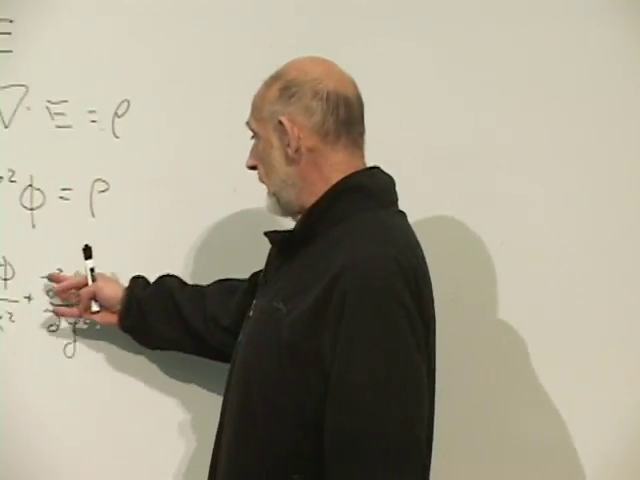
\includegraphics[width=0.70\textwidth]{lecture_08_figure_02.png}
  \caption{完整的柯西--黎曼方程組，包含相對的負號。}
  \lectureframe{00:19:48}
  \label{fig:l08-cr-board}
\end{figure}

本講也簡要區分幾個相關術語。在整個有限複平面上全純的函數稱為整函數；亞純函數則可以有孤立極點。因此，\(1/z\)在\(z=0\)之外解析，但不是整函數。

\section{調和共軛與共形幾何}

柯西--黎曼方程是耦合的一階方程，但它們也蘊含各自的二階方程。將\(\partial_xu=\partial_yv\)對\(x\)微分，將\(\partial_yu=-\partial_xv\)對\(y\)微分，再把兩式相加：
\begin{align}
  \partial_x^2u&=\partial_x\partial_yv,\\
  \partial_y^2u&=-\partial_y\partial_xv,\\
  \therefore\qquad
  \partial_x^2u+\partial_y^2u&=0.
  \label{eq:l08-harmonic-u}
\end{align}
交換\(u\)與\(v\)後重複同一論證，可得
\begin{equation}
  \partial_x^2v+\partial_y^2v=0.
  \label{eq:l08-harmonic-v}
\end{equation}
因此，解析函數的實部與虛部互為調和共軛。任意兩個調和函數不會自動組成解析函數；兩者仍須滿足\eqref{eq:l08-cauchy-riemann}所給的關係。

\begin{figure}[H]
  \centering
  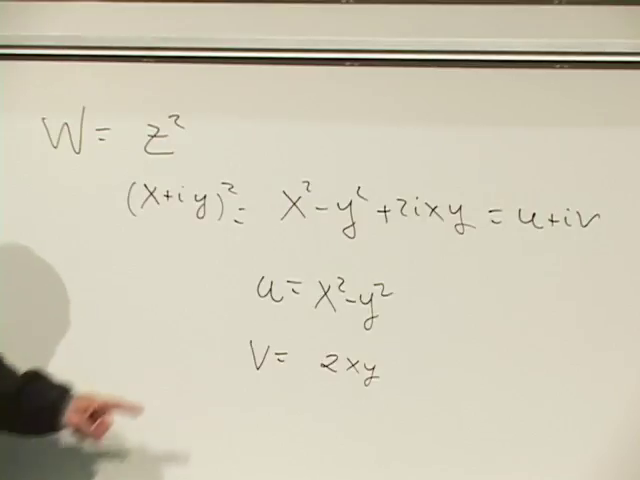
\includegraphics[width=0.68\textwidth]{lecture_08_figure_03.png}
  \caption{混合偏導數相消後，解析映射的一個分量便滿足拉普拉斯方程。}
  \lectureframe{00:23:09}
  \label{fig:l08-harmonic-board}
\end{figure}

還可以用向量來理解。若\(\mathbf F=(u,-v)\)，則兩個柯西--黎曼方程表示，在所採用的定向慣例下，\(\mathbf F\)的散度與二維旋度都為零。這就回到了靜電學。

\subsection{為何角度會保持不變}

將兩個微小的複位移寫成極式：
\begin{equation}
  \delta z=\rho e^{i\theta},
  \qquad
  \Delta z=\rho'e^{i\theta'}.
\end{equation}
兩者的比值相位為\(\theta-\theta'\)，恰好就是它們之間的夾角。在解析映射下，
\begin{equation}
  \frac{\delta w}{\delta z}
  =\frac{\Delta w}{\Delta z}
  =w'(z),
\end{equation}
因為導數與方向無關。重新整理可得
\begin{equation}
  \frac{\Delta z}{\delta z}
  =\frac{\Delta w}{\delta w}.
  \label{eq:l08-angle-ratio}
\end{equation}
等式兩側的相位相同，因此原來兩個線段的夾角，等於其映像之間的夾角。

\begin{figure}[H]
  \centering
  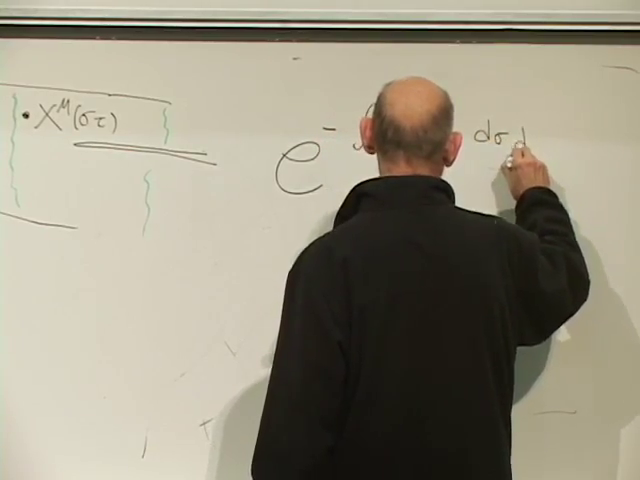
\includegraphics[width=0.70\textwidth]{lecture_08_figure_04.png}
  \medskip

  \begin{tikzpicture}[x=0.9cm,y=0.9cm,>=Latex]
    \begin{scope}
      \draw[->] (-0.2,0) -- (2.3,0);
      \draw[->] (0,-0.2) -- (0,2.1);
      \draw[very thick,blue!65!black,->] (0,0) -- (1.85,0.45)
        node[right] {\(\delta z\)};
      \draw[very thick,orange!75!black,->] (0,0) -- (0.72,1.65)
        node[above] {\(\Delta z\)};
      \draw (0.58,0.14) arc[start angle=14,end angle=66,radius=0.60];
      \node at (1.0,-0.55) {\(z\)-plane};
    \end{scope}
    \draw[->,thick] (3.0,0.9) -- (4.2,0.9)
      node[midway,above] {\(w(z)\)};
    \begin{scope}[xshift=5.0cm]
      \draw[->] (-0.2,0) -- (2.3,0);
      \draw[->] (0,-0.2) -- (0,2.1);
      \draw[very thick,blue!65!black,->] (0,0) -- (1.65,0.70)
        node[right] {\(\delta w\)};
      \draw[very thick,orange!75!black,->] (0,0) -- (0.48,1.62)
        node[above] {\(\Delta w\)};
      \draw (0.54,0.23) arc[start angle=23,end angle=74,radius=0.59];
      \node at (1.0,-0.55) {\(w\)-plane};
    \end{scope}
  \end{tikzpicture}
  \caption{黑板上的證明與清楚的局部重構。乘以\(w'(z)\)會讓每個無窮小方向都旋轉並縮放相同的量，因此相對角度保持不變。}
  \lectureframe{00:34:11}
  \label{fig:l08-angle-proof}
\end{figure}

這個局部論證假設\(w'(z)\neq0\)。在臨界點，映射可能不再是局部一對一，必須另行分析其幾何。離開這類點時，解析映射與保向的共形映射在局部上是同一類映射。

\section{幫助培養直覺的例子}

\subsection{平方映射與複共軛}

對於\(w=z^2\)，
\begin{equation}
  (x+iy)^2=x^2-y^2+2ixy=u+iv,
\end{equation}
因此
\begin{equation}
  u=x^2-y^2,
  \qquad
  v=2xy.
  \label{eq:l08-z-squared-components}
\end{equation}
\(u\)的二階導數為\(2\)與\(-2\)；\(v\)的二階導數則各自為零。兩者都是調和函數，直接微分也可驗證柯西--黎曼方程。

\begin{figure}[H]
  \centering
  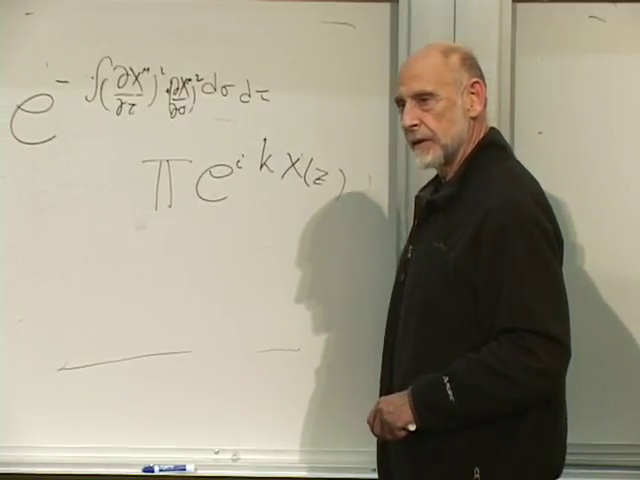
\includegraphics[width=0.72\textwidth]{lecture_08_figure_05.png}
  \caption{平方映射分解成實部與虛部兩個調和分量。}
  \lectureframe{00:36:45}
  \label{fig:l08-z-square-board}
\end{figure}

\begin{classroomqa}
\audiencequestion{\(1/z\)是非解析函數的例子嗎？
\lecturetimestamp{00:37:49}}
\lecturerresponse{只在一個點有問題。它在\(z\neq0\)處解析，而在原點有極點。若要看一個處處不滿足柯西--黎曼檢驗的映射，複共軛是更好的例子。}
\end{classroomqa}

相較之下，
\begin{equation}
  w=\bar z=x-iy
  \qquad\Longrightarrow\qquad
  u=x,\quad v=-y
\end{equation}
會反轉定向。它的導數因符號相反而不滿足第一個柯西--黎曼方程，因此它不是以\(z\)為自變數的解析函數。

\begin{figure}[H]
  \centering
  \includegraphics[width=0.62\textwidth]{lecture_08_figure_06.png}
  \caption{複共軛是刻意選用的非解析反例。}
  \lectureframe{00:38:38}
  \label{fig:l08-conjugate-board}
\end{figure}

\subsection{指數函數及其反函數}

\begin{classroomqa}
\audiencequestion{若\(e^z\)是解析函數，為何它的反函數\(\log z\)也應該是解析函數？\lecturetimestamp{00:40:38}}
\lecturerresponse{在反函數存在且\(w'(z)\neq0\)的地方，它的導數為\(1/w'(z)\)。因此，導數仍與方向無關。對數函數在整體上是多值的，所以必須選定一個分支，並排除其分支點與分支切線。在選定的區域內，局部共形的敘述仍然成立。}
\end{classroomqa}

尤拉公式給出
\begin{equation}
  w=e^z=e^{x+iy}
  =e^x(\cos y+i\sin y),
\end{equation}
因此
\begin{equation}
  u=e^x\cos y,
  \qquad
  v=e^x\sin y.
  \label{eq:l08-exponential-components}
\end{equation}
例如，\(\partial_xu=e^x\cos y=\partial_yv\)，第二個柯西--黎曼方程也可同樣直接得到。

\begin{figure}[H]
  \centering
  \includegraphics[width=0.68\textwidth]{lecture_08_figure_07.png}
  \caption{指數映射的實部與虛部。}
  \lectureframe{00:42:23}
  \label{fig:l08-exponential-board}
\end{figure}

\section{半平面、帶狀區域、圓柱與圓盤}

\subsection{對數將半徑轉為時間}

取右半平面，其中\(-\pi/2<\theta<\pi/2\)，並令
\begin{equation}
  z=re^{i\theta},
  \qquad
  w=\log z=\log r+i\theta.
  \label{eq:l08-log-map}
\end{equation}
右半平面便映到無限延伸的帶狀區域
\begin{equation}
  -\frac{\pi}{2}<\operatorname{Im}w<\frac{\pi}{2}.
\end{equation}
固定\(\theta\)的射線會變成水平線，固定\(r\)的半圓則會變成垂直線。原點映到\(\operatorname{Re}w=-\infty\)，而\(r=\infty\)映到\(\operatorname{Re}w=+\infty\)。

\begin{figure}[H]
  \centering
  \includegraphics[width=0.75\textwidth]{lecture_08_figure_08.png}
  \caption{對數將右半平面映入無限延伸的帶狀區域：極射線與半圓變成互相垂直的矩形網格。}
  \lectureframe{00:47:48}
  \label{fig:l08-log-strip-board}
\end{figure}

帶狀區域是開弦的標準世界面。有限範圍的座標是沿著弦的參數，而沿無限延伸方向的平移則代表世界面時間。透過反指數映射，時間平移會變成縮放\(z\mapsto e^a z\)。因此，同一個對稱性在帶狀區域中表現為平移，在半平面中則表現為均勻膨脹。

\begin{classroomqa}
\audiencequestion{像\(r=1\)這樣的特定值會映到哪裡？帶狀區域上的座標仍然是極座標嗎？\lecturetimestamp{00:50:58}}
\lecturerresponse{固定半徑的圓會變成\(\operatorname{Re}w=\log r\)處的垂直線；尤其是，\(r=1\)會映到中心線\(\operatorname{Re}w=0\)。極座標描述的是\(z\)平面；\(w\)平面則使用一般的直角座標\((\log r,\theta)\)。}
\end{classroomqa}

若以\(\log z\)映射整個穿孔平面，角座標的週期為\(2\pi\)。因此，所得帶狀區域的上、下邊緣會相互識別，形成無限長圓柱。帶有邊界的半平面描述開弦世界面；沒有邊界且角度具有週期性的整個平面，則描述閉弦圓柱。

\begin{figure}[H]
  \centering
  \includegraphics[width=0.75\textwidth]{lecture_08_figure_09.png}
  \caption{半平面與帶狀區域的圖像，以及將整個穿孔平面變成閉弦圓柱的週期性識別。}
  \lectureframe{00:54:23}
  \label{fig:l08-open-closed-board}
\end{figure}

\subsection{映至單位圓盤的凱萊映射}

線性分式映射，又稱莫比烏斯映射，可將右半平面映至單位圓盤：
\begin{equation}
  w=\frac{z-1}{z+1}.
  \label{eq:l08-cayley}
\end{equation}
它將\(z=0\)映至\(-1\)，將\(z=\infty\)映至\(+1\)，並將虛軸映至\(|w|=1\)。若\(z=ir\)，則
\begin{equation}
  \left|\frac{ir-1}{ir+1}\right|=1.
\end{equation}
滿足\(\operatorname{Re}z>0\)的點會映到圓內；左半平面則映到圓外。
\editorialnote{在現場推導中，描述圓盤內部映像時寫下了倒數\((z+1)/(z-1)\)。這個倒數有相同的單位圓邊界，但會將右半平面映到圓外。方程\eqref{eq:l08-cayley}採用的是與所述幾何相符的圓盤內部慣例。}

\begin{figure}[H]
  \centering
  \includegraphics[width=0.72\textwidth]{lecture_08_figure_10.png}
  \caption{構造單位圓邊界的線性分式映射。黑板上出現的倒數形式會交換圓內與圓外。}
  \lectureframe{00:58:38}
  \label{fig:l08-cayley-board}
\end{figure}

莫比烏斯映射會將廣義圓（包括直線）映成廣義圓。因此，半平面上的徑向線與圓弧網格，在圓盤上會變成兩族互相垂直的弧。直徑只是圓心趨於無窮遠時的圓弧極限。

\begin{classroomqa}
\audiencequestion{圓盤內畫出的弧真的都是圓嗎？
\lecturetimestamp{01:00:55}}
\lecturerresponse{是的。它們的圓心各不相同，而且常在可見圓盤之外。直徑就是同一族圓的半徑趨於無窮大時的極限。}
\end{classroomqa}

\begin{classroomqa}
\audiencequestion{圖中的圓盤代表球面嗎？另一個半平面映到哪裡？\lecturetimestamp{01:01:21}}
\lecturerresponse{這裡畫的是平面圓盤，不是球面。右半平面映到圓的內部，左半平面則映到圓外。若將無窮遠點加入整個複平面，擴充後的平面可透過球極投影表示為球面；那是另一個整體性的敘述。}
\end{classroomqa}

\begin{classroomqa}
\audiencequestion{圓盤中的哪些曲線對應於原本的徑向線與等半徑半圓？\lecturetimestamp{01:02:59}}
\lecturerresponse{正實軸會變成連接\(-1\)與\(+1\)的直徑。其他射線會變成連接這兩個邊界點的圓弧。等半徑半圓則變成另一族互相垂直、兩端落在單位圓上的曲線。}
\end{classroomqa}

\begin{figure}[H]
  \centering
  \includegraphics[width=0.72\textwidth]{lecture_08_figure_11.png}
  \caption{半平面中的直線與半圓，在圓盤中變成互相垂直的圓弧與直線族。}
  \lectureframe{01:03:48}
  \label{fig:l08-circle-grid-board}
\end{figure}

\section{四弦世界面}

現在回到散射。兩條開弦入射，合併成一條弦，傳播一段任意長的時間，再分裂成兩條出射弦。在帶狀座標中，世界面看起來像一條長帶子，兩端各開有一道縫---這就是「運動繃帶」的圖像。中間態的存續時間並非預先選定，而是振幅積分所涵蓋的各種歷程之一。

令\((\sigma,\tau)\)為世界面上的座標，並令
\begin{equation}
  X^\mu=X^\mu(\sigma,\tau)
  \label{eq:l08-embedding}
\end{equation}
表示世界面在時空中的位置。標記\(\sigma,\tau\)位於二維參數曲面上；指標\(\mu\)則標示時空座標。在玻色弦理論中，\(\mu=0,\ldots,25\)；超弦理論則有十個時空座標。

經過 Wick 轉動後，自由嵌入場的歐幾里得作用量為
\begin{equation}
  S_E[X]
  =\frac{1}{4\pi\alpha'}\int_\Sigma d\sigma\,d\tau\,
  \left[
    \partial_\tau X^\mu\partial_\tau X_\mu
    +\partial_\sigma X^\mu\partial_\sigma X_\mu
  \right].
  \label{eq:l08-euclidean-action}
\end{equation}
相應的路徑積分會對所選世界面嵌入時空的所有方式求和：
\begin{equation}
  \int\mathcal D X\,e^{-S_E[X]}.
  \label{eq:l08-bare-worldsheet-integral}
\end{equation}

\begin{figure}[H]
  \centering
  \includegraphics[width=0.74\textwidth]{lecture_08_figure_12.png}
  \caption{完整且為正的歐幾里得世界面權重。兩個導數項都對所有時空分量求和。}
  \lectureframe{01:11:34}
  \label{fig:l08-action-board}
\end{figure}

帶縫的條帶只有一個連通邊界。因此，利用共形自由度，可以將它表示為圓盤。條帶的四個遠端會變成邊界上的四個標記點。移動這些標記點會改變條帶座標中合併與分裂看起來相隔多遠，但不會改變底層曲面或物理內容。

\begin{figure}[H]
  \centering
  \includegraphics[width=0.76\textwidth]{lecture_08_figure_13.png}
  \caption{帶縫條帶世界面及其圓盤表示，外部弦對應到圓盤邊界上的點。}
  \lectureframe{01:15:18}
  \label{fig:l08-bandage-disc-board}
\end{figure}

用來描繪此共形映射的細部網格線沒有物理意義。重要的是拓撲、邊界和代表外部態的標記點。同一個世界面可以拉伸成不同的通道圖像，而無須引入新的交互作用。

\section{外部態作為邊界插入}

裸積分\eqref{eq:l08-bare-worldsheet-integral}尚未說明哪些動量入射、哪些動量出射。對動量為\(k_i^\mu\)的純量開弦態，在邊界上插入頂點算符
\begin{equation}
  V_i(z_i)=e^{\,i k_i\cdot X(z_i)},
  \qquad
  k_i\cdot X=k_{i\mu}X^\mu.
  \label{eq:l08-vertex}
\end{equation}
點\(z_i\)是世界面邊界上的位置；它不是時空座標，也不代表動量方向。

\begin{figure}[H]
  \centering
  \includegraphics[width=0.72\textwidth]{lecture_08_figure_14.png}
  \caption{體內的歐幾里得權重與邊界動量插入的乘積分別列為不同因子。}
  \lectureframe{01:18:58}
  \label{fig:l08-vertex-board}
\end{figure}

對\(n\)條外部開弦，示意性的散射處方為
\begin{equation}
  \begin{aligned}
    \mathcal A_n(k_1,\ldots,k_n)
    &=\int_{\mathcal M_{0,n}^{\partial}}\!d\mu(z_i)
      \int\mathcal D X\\
    &\quad\times e^{-S_E[X]}
      \prod_{i=1}^{n}e^{\,i k_i\cdot X(z_i)}.
  \end{aligned}
  \label{eq:l08-open-string-prescription}
\end{equation}
泛函積分是對嵌入場\(X^\mu\)進行；有限維積分則是對彼此不等價的邊界插入位置進行。此處省略了極化因子與規範固定測度，講課時也同樣省略。
\editorialnote{完整的規範固定弦振幅還包含相應的鬼場貢獻、依態而定的頂點因子、耦合常數及歸一化。方程\eqref{eq:l08-open-string-prescription}記錄的是本講所推導的嵌入場與位置依賴性。}

\begin{classroomqa}
\audiencequestion{既然外部動量固定，為什麼還要對它們積分？\lecturetimestamp{01:20:42}}
\lecturerresponse{外部動量並沒有被積分。\(k_i\)是散射振幅中的固定標記。被積分的是嵌入場，以及插入這些固定動量的世界面位置\(z_i\)。後者的積分取代了條帶圖像中對中間態存續時間的積分。}
\end{classroomqa}

\begin{classroomqa}
\audiencequestion{頂點因子的乘積放在路徑積分內；它是作用量的一部分嗎？\lecturetimestamp{01:21:39}}
\lecturerresponse{這些因子乘在泛函積分中的\(e^{-S_E}\)上。也可以把因子等價地併入指數，視為加入作用量的局域源項；不過在概念上，它們是頂點算符，而非自由的體作用量的一部分。}
\end{classroomqa}

\begin{figure}[H]
  \centering
  \includegraphics[width=0.76\textwidth]{lecture_08_figure_15.png}
  \caption{以彼此分開的因子\(e^{ik_i\cdot X(z_i)}\)表示每個外部粒子的路徑積分。}
  \lectureframe{01:23:23}
  \label{fig:l08-full-prescription-board}
\end{figure}

\begin{classroomqa}
\audiencequestion{世界面 Wick 轉動後，\(e^{ik\cdot X}\)為什麼仍含有\(i\)？\lecturetimestamp{01:23:42}}
\lecturerresponse{轉動改變的是世界面時間，並將體內權重從\(e^{iS}\)轉為\(e^{-S_E}\)。動量本徵函數中的\(i\)則是標記時空動量的傅立葉相位，作用不同，因此仍然保留。}
\end{classroomqa}

\begin{classroomqa}
\audiencequestion{位置\(z_i\)會決定動量向量的方向嗎？\lecturetimestamp{01:24:19}}
\lecturerresponse{不會。方向由時空分量\(k_i^\mu\)表示。插入點\(z_i\)說明該動量在世界面描述中的插入位置；\(X^\mu(z_i)\)則是由\(\mathcal D X\)所求和的場值之一。}
\end{classroomqa}

\begin{classroomqa}
\audiencequestion{圖中繃帶兩端的傾斜角度，代表物理動量的方向嗎？\lecturetimestamp{01:25:07}}
\lecturerresponse{不代表。繃帶描繪的是參數空間，不是弦在物理時空中的形狀。兩端可以畫成水平、傾斜，或經共形變換而彎曲。物理方向由分量\(k^\mu\)表示，而\(X^\mu(\sigma,\tau)\)則是積分變數。}
\end{classroomqa}

\section{高斯積分與靜電學}

作用量\eqref{eq:l08-euclidean-action}對每個\(X^\mu\)分量都是二次的；將插入算符的指數因子與作用量合併後，插入便形成線性源。因此，泛函積分是高斯積分。在鞍點處，每個時空分量都滿足泊松方程，其示意形式為
\begin{equation}
  \nabla^2 X^\mu(z)
  \propto
  i\alpha'\sum_i k_i^\mu\,\delta(z-z_i),
  \label{eq:l08-electrostatic-source}
\end{equation}
並在圓盤邊界上滿足開弦的邊界條件。每個\(X^\mu\)都像是各自獨立的靜電位勢，而每個動量分量\(k_i^\mu\)則像是置於\(z_i\)的相應電荷。

\begin{figure}[H]
  \centering
  \includegraphics[width=0.76\textwidth]{lecture_08_figure_16.png}
  \caption{帶有邊界源的圓盤，可解讀為每個時空分量各自對應一個獨立的二維靜電問題。}
  \lectureframe{01:28:58}
  \label{fig:l08-electrostatic-disc-board}
\end{figure}

先解出靜電問題並計算其能量，再取負能量的指數，最後對彼此不等價的電荷位置積分。在標準開弦歸一化下，嵌入場的關聯函數給出 Koba--Nielsen 因子
\begin{equation}
  \left\langle\prod_i e^{\,ik_i\cdot X(z_i)}\right\rangle
  \propto
  (2\pi)^D\delta^{(D)}\!\left(\sum_i k_i\right)
  \prod_{i<j}|z_i-z_j|^{2\alpha' k_i\cdot k_j}.
  \label{eq:l08-koba-nielsen}
\end{equation}
狄拉克 delta 函數表示動量守恆。乘積中的各項包含成對的靜電能。對於此處使用的四個純量邊界插入，固定三個位置後，剩下的積分便化為前幾講介紹過的尤拉 beta 積分。

\begin{classroomqa}
\audiencequestion{靜電能是有二十六個，還是只有一個？
\lecturetimestamp{01:30:53}}
\lecturerresponse{每個時空分量都對應一個獨立的位勢與電場。在正交歸一的靶空間基底中，各分量的二次能量沒有交叉項；取指數之前，所有貢獻會先加總成一個總作用量。}
\end{classroomqa}

\begin{classroomqa}
\audiencequestion{圓盤上的角座標就是物理散射角嗎？\lecturetimestamp{01:32:10}}
\lecturerresponse{不是。它是世界面上的位置參數。其不等價組合與中間傳播時間有關，並且需要積分。物理散射角則由固定動量所構成的洛侖茲不變量來表示。}
\end{classroomqa}

\begin{classroomqa}
\audiencequestion{為什麼這個構造在臨界維度以外會失效？
\lecturetimestamp{01:32:35}}
\lecturerresponse{形式上的高斯積分並不足以確保理論一致。規範固定會引入共形反常；只有在臨界維度，物質場與鬼場的貢獻才會相消：玻色弦為\(D=26\)，超弦為\(D=10\)。若未能相消，量子世界面所假設的共形對稱性便會消失。}
\end{classroomqa}

\begin{classroomqa}
\audiencequestion{我們是否已經假設有三個宏觀空間維度，以及緊緻化的額外維度？\lecturetimestamp{01:33:38}}
\lecturerresponse{沒有，這個構造尚未涉及緊緻化。在此階段，玻色弦的座標仍涵蓋靶空間的全部二十六個方向；超弦則涵蓋十個方向。如何讓其中一部分維度在宏觀尺度上保持廣延，會在接下來的討論中說明。}
\end{classroomqa}

\begin{classroomqa}
\audiencequestion{這裡與靜電學的關聯，是否只在於座標滿足拉普拉斯方程？\lecturetimestamp{01:33:57}}
\lecturerresponse{正是如此。在插入點以外，每個\(X^\mu\)都是調和的；頂點算符則提供 delta 函數源。無論是否使用靜電學的說法，這在數學上都與帶有點電荷的靜態二維位勢邊值問題相同。}
\end{classroomqa}

\subsection{共形冗餘與模數的數目}

圓盤的共形自同構群有三個實參數，為\(\mathrm{PSL}(2,\mathbb R)\)。因此，可以將三個有序的邊界點固定在方便的位置。對於四條外部弦，只剩第四個位置需要積分；對於\(n\)個有序邊界插入，樹圖階的實位置積分有
\begin{equation}
  n-3
  \label{eq:l08-n-minus-three}
\end{equation}
個。

\begin{classroomqa}
\audiencequestion{圓盤周圍有四個彼此獨立的角位置嗎？\lecturetimestamp{01:34:37}}
\lecturerresponse{物理上並非如此。起初雖然寫下四個位置，但圓盤的共形對稱性可以把任意三個位置選在方便之處。對於兩條入射、兩條出射的振幅，只剩第四個位置相對於其他位置的關係需要考慮。}
\end{classroomqa}

\begin{figure}[H]
  \centering
  \includegraphics[width=0.72\textwidth]{lecture_08_figure_17.png}
  \caption{圓盤上的四個邊界插入。共形自由度可固定任意三個位置，留下四點的一個模數。}
  \lectureframe{01:35:18}
  \label{fig:l08-fix-three-board}
\end{figure}

\begin{classroomqa}
\audiencequestion{如果條帶圖中的兩個分裂點不在同一高度，會怎樣？\lecturetimestamp{01:35:24}}
\lecturerresponse{共形映射可以消除這種表面上的高度差異。不同圖像只是同一模數的不同座標表示。真正不變的積分是對剩餘邊界位置積分，也等價於對傳播時間積分。}
\end{classroomqa}

\begin{classroomqa}
\audiencequestion{外部粒子更多時，還剩下多少個位置參數？\lecturetimestamp{01:36:00}}
\lecturerresponse{利用共形對稱性固定三個插入點，再對其餘\(n-3\)個位置積分。這就是有序樹圖階開弦振幅的邊界模數計數。}
\end{classroomqa}

\begin{classroomqa}
\audiencequestion{這和 M 理論有什麼關係？
\lecturetimestamp{01:36:37}}
\lecturerresponse{目前還沒有。這裡討論的是世界面上的微擾開弦散射。它與 M 理論的關係需要借助後續的對偶性與非微擾觀念，因此這個問題留待之後討論。}
\end{classroomqa}

\begin{classroomqa}
\audiencequestion{不同的垂直或交叉條帶圖示，代表不同的計算嗎？\lecturetimestamp{01:36:49}}
\lecturerresponse{不是。可以固定一個方便的點，讓其餘模數在完整的區間內變化。條帶圖示與圓盤上的邊界點積分，是同一積分的不同切片方式；因此，所有外部弦都能以對稱的方式處理。}
\end{classroomqa}

\section{此處方尚未解決的問題}

圓盤公式可直接推廣至更多外部弦：加入更多頂點算符，並對其 \(n-3\) 個互不等價的邊界位置積分。這是針對自洽弦模型的精確樹級處方，但還不是描述已觀測粒子物理的現實模型。簡單的玻色弦理論有錯誤的時空維度，並存在其他物理缺陷。超弦改善了粒子譜，並將臨界維度降至十維，但仍須將六個空間維度緊緻化。

\begin{classroomqa}
\audiencequestion{這個簡單模型已經符合粒子碰撞實驗嗎？\lecturetimestamp{01:39:06}}
\lecturerresponse{還沒有。它的共振結構在歷史上與強子散射相似，但二十六維玻色弦模型無法直接描述已觀測到的粒子。這套形式架構為該模型定義了散射振幅；若要符合自然界，還需要現實的粒子譜、緊緻化、交互作用以及真空選擇。}
\end{classroomqa}

\begin{classroomqa}
\audiencequestion{緊緻化能縮減額外維度，並產生符合現實的粒子資料嗎？\lecturetimestamp{01:41:10}}
\lecturerresponse{緊緻化可以降低有效的宏觀維度，並產生粒子譜與規範群。許多數學上的真正困難也由此而來。已有許多自洽的緊緻化方案，但如何選出唯一能描述已觀測基本粒子的模型，仍未有定論。}
\end{classroomqa}

本講強調這項區別，而非宣稱理論已經完成。弦論構造在數學上有明確定義，也為引力與幾何帶來深刻的成果；然而，這些構造的多樣性本身也是物理問題的一部分。

\begin{classroomqa}
\audiencequestion{有沒有簡單的方法可以記住玻色弦的臨界維度為何是二十六？\lecturetimestamp{01:43:19}}
\lecturerresponse{先前的振子計算使用了正則化的零點能總和 \(1+2+3+\cdots=-1/12\)。橫向振子的貢獻涉及二十四個方向；加回兩個縱向時空座標後，便得到 \(24+2=26\)。這只是幫助記憶先前一致性論證的提示，並非在此提出新的推導。}
\end{classroomqa}

\begin{classroomqa}
\audiencequestion{插入的動量 \(k_i\) 本身是量子化的嗎？\lecturetimestamp{01:43:46}}
\lecturerresponse{在非緊緻時空中，動量的分量是連續的。量子化的是振子能級，因此允許的質量平方譜也是量子化的。緊緻維度可能使相應的動量分量與繞行數分量量子化，但這部分留待下一節討論。}
\end{classroomqa}

\chapter{弦、引力、緊緻化與 T 對偶}

\lectureoverview{點粒子幾乎可以在任何光滑幾何上自洽地運動，量子弦卻不行。弦有無窮多個零點振盪，會逐步探測靶空間中愈來愈短的尺度；隨著這些振盪逐一納入，有效幾何也會改變。要求這個過程達到不動點，便得到\(R_{\mu\nu}=0\)，也就是真空愛因斯坦方程。接著，我們從這項一致性條件轉向緊緻化。一個圓同時具有 Kaluza--Klein 動量態與弦的纏繞態；將兩者互換，半徑為\(R\)的圓便與半徑為\(\alpha'/R\)的圓等價。}

\section{作為選擇原理的一致性}

有兩個問題需要回答：為什麼弦理論中會有引力？為什麼弦理論比點粒子力學嚴格得多？這其實是同一個問題。背景幾何只有在弦能於其中傳播，且結果不會任意依賴我們對弦分辨得多精細時，才是可接受的。

先看一個對照問題：受限於光滑彎曲曲面上的點粒子。經典情況下，它沿著測地線運動；測地線是直線在曲面內部的對應概念。我們可以用許多短線段近似其運動，寫出差分方程，再令線段長度趨近於零。所得常微分方程具有明確的連續極限。

量子力學改變的是對歷史的求和方式，結論卻不變。我們不再選定一條經典路徑，而是對曲面上的路徑求振幅總和。時間同樣可以切分成許多小步；取極限後，也可以用彎曲位形空間上的Schr\"odinger方程來描述。對光滑曲面而言，這個極限會收斂到確定的傳播子與能譜。

\begin{figure}[H]
  \centering
  \includegraphics[width=0.72\textwidth]{lecture_09_figure_01.png}
  \caption{曲面上的光滑路徑，以及時間切片量子求和所涵蓋的鋸齒狀路徑。兩者都位於靶曲面上，並由其內在幾何描述。}
  \lectureframe{00:05:10}
  \label{fig:l09-particle-paths}
\end{figure}

\begin{classroomqa}
\audiencequestion{在路徑積分中，是否所有路徑都必須留在曲面上？\lecturetimestamp{00:05:39}}
\lecturerresponse{是。曲面就是粒子的位形空間，不是嵌在更大空間中的薄片，讓粒子可以穿過外部空間抄近路。每個中間點都必須位於曲面上，所有長度與作用量都以曲面的內在度規計算。}
\end{classroomqa}

對弦而言，相應的問題更難。弦不能只用質心位置來描述；它還有無窮多個振子模。因此，提高解析度也就意味著納入更多動力學自由度。只有在逐步納入這些振子模時，觀測量仍趨近某個極限，理論才是一致的。

\section{球面上的點粒子}

球面是最簡單的彎曲測試幾何。設球面半徑為\(R\)，先將質量為\(m\)的粒子放在球面上。若粒子沿大圓運動，
\begin{equation}
  E=\frac{1}{2}mv^2=\frac{p^2}{2m},
  \qquad
  L=pR.
  \label{eq:l09-particle-energy}
\end{equation}
因此，
\begin{equation}
  E=\frac{L^2}{2mR^2}
   =\frac{L^2}{2I},
  \qquad
  I=mR^2.
  \label{eq:l09-rotor-energy}
\end{equation}
半徑透過轉動慣量進入計算。將角動量量子化後，便得到熟悉的剛性轉子能譜，而且完全不需要紫外截斷。

\begin{figure}[H]
  \centering
  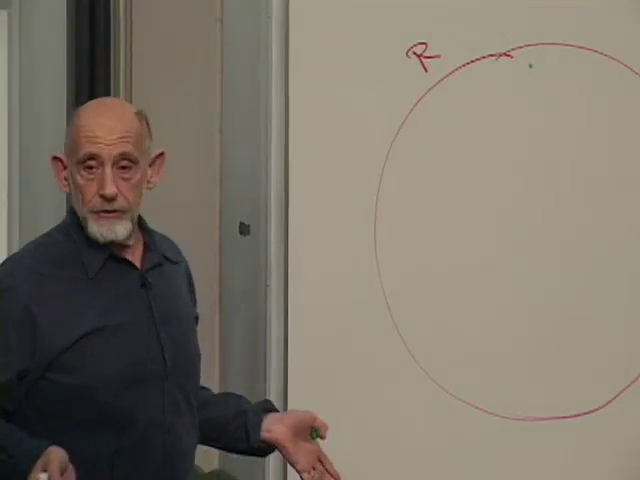
\includegraphics[width=0.74\textwidth]{lecture_09_figure_02.png}
  \caption{點粒子的對照計算：\(p^2/(2m)=L^2/(2mR^2)=L^2/(2I)\)。}
  \lectureframe{00:11:25}
  \label{fig:l09-sphere-rotor}
\end{figure}

這個毫無困難的例子很重要。問題不在曲率本身，而是在曲率與弦的量子內部延展性耦合時才會出現。

\section{真空中的弦並非點狀}

考慮開弦的一個橫向座標，並扣除質心位置。這裡採用的振子展開式僅為示意：
\begin{equation}
  X(\sigma)-X_{\mathrm{cm}}
  \sim
  \sum_{n=1}^{\infty}
  \frac{a_n+a_n^\dagger}{\sqrt n}\cos(n\sigma).
  \label{eq:l09-mode-expansion}
\end{equation}
關鍵成分是餘弦模、振子算符，以及因子\(1/\sqrt n\)。在討論尺寸時，精確的歸一化並不重要。
\editorialnote{精確展開式還包含依約定而定的\(\alpha'\)因子、數值常數，以及不同的振子記號。方程\eqref{eq:l09-mode-expansion}只保留紫外估算所需的依賴關係，與黑板上的推導相同。}

\begin{figure}[H]
  \centering
  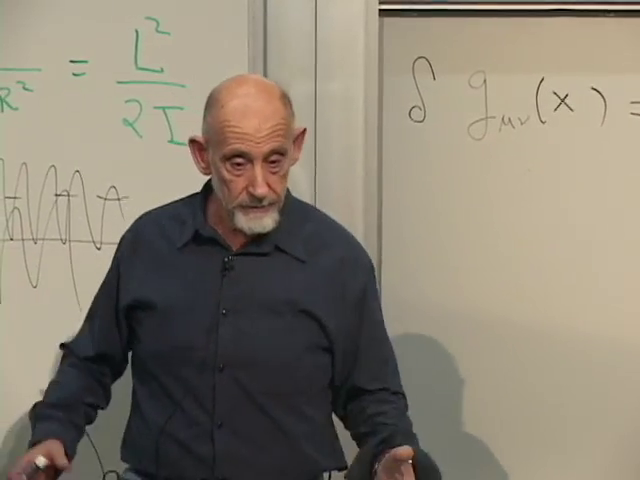
\includegraphics[width=0.78\textwidth]{lecture_09_figure_03.png}
  \caption{振子展開的結構，以及將其平方後得到的雙重求和。}
  \lectureframe{00:15:20}
  \label{fig:l09-string-modes}
\end{figure}

在振子真空態中，相對於質心的距離平方為
\begin{align}
  \expect{\bigl(X(\sigma)-X_{\mathrm{cm}}\bigr)^2}_0
  &\sim
  \sum_{n,m\geq1}
  \frac{\cos(n\sigma)\cos(m\sigma)}{\sqrt{nm}}\notag\\
  &\qquad\times
  \bra{0}(a_n+a_n^\dagger)\notag\\
  &\hspace{6em}\times(a_m+a_m^\dagger)\ket{0}.
  \label{eq:l09-size-double-sum}
\end{align}
大多數項都會消失：兩個湮滅算符作用於右矢後為零；兩個產生算符作用後所得的態與左矢正交；依此排序，先產生再湮滅的算符組合，其真空期望值也為零。剩下的收縮項為
\begin{equation}
  \bra{0}a_n a_m^\dagger\ket{0}=\delta_{nm}.
  \label{eq:l09-vacuum-contraction}
\end{equation}

\begin{figure}[H]
  \centering
  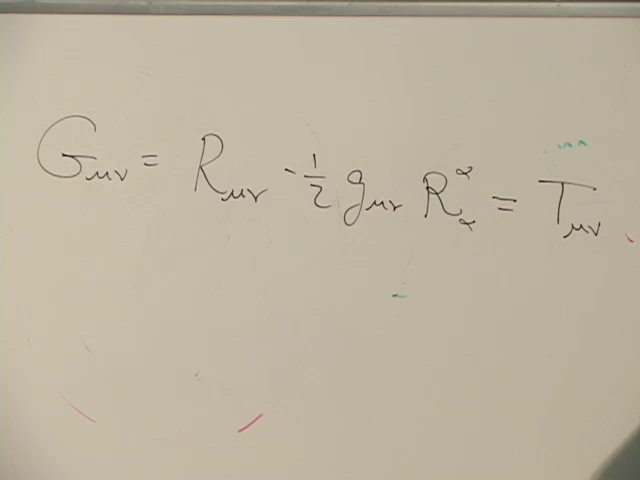
\includegraphics[width=0.74\textwidth]{lecture_09_figure_04.png}
  \caption{剩下的真空收縮使雙重振子求和化為單一求和。}
  \lectureframe{00:20:10}
  \label{fig:l09-vacuum-contraction}
\end{figure}

因此
\begin{equation}
  \expect{\bigl(X(\sigma)-X_{\mathrm{cm}}\bigr)^2}_0
  \sim
  \sum_{n=1}^{\infty}\frac{\cos^2(n\sigma)}{n}.
  \label{eq:l09-size-single-sum}
\end{equation}
在弦上的一般位置，或對\(\sigma\)取平均後，\(\cos^2(n\sigma)\)的貢獻約為\(1/2\)。若模式截斷為\(N\)，則
\begin{equation}
  \expect{\bigl(X-X_{\mathrm{cm}}\bigr)^2}_{0,N}
  \sim
  \frac{1}{2}\sum_{n=1}^{N}\frac{1}{n}
  =\frac{1}{2}\log N+O(1).
  \label{eq:l09-logarithmic-size}
\end{equation}

\begin{figure}[H]
  \centering
  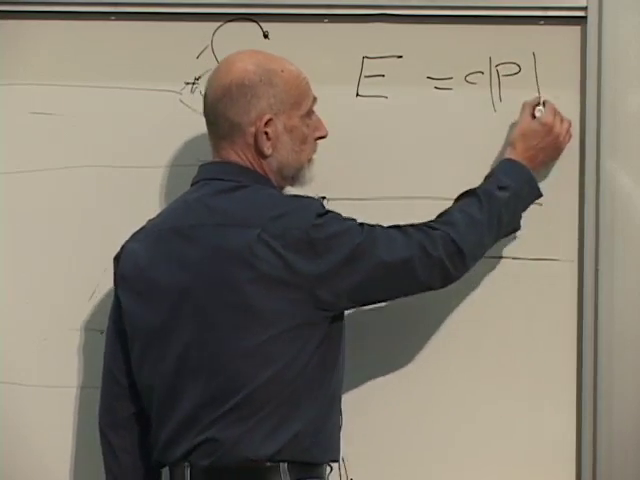
\includegraphics[width=0.72\textwidth]{lecture_09_figure_05.png}
  \caption{黑板上的推導得到控制基態展寬的調和級數。}
  \lectureframe{00:22:05}
  \label{fig:l09-harmonic-size}
\end{figure}

例如只保留前二十五個模式，會得到一個有限但模糊的物體；然而它還不是連續弦。移除截斷後，均方展寬會按對數增長。這不代表平直空間中的弦理論不一致。在平直空間中，質心運動與振子運動彼此分離，而物理振幅中的精細抵消會維持預期的局域性。尺寸增長是一項警訊；曲率則告訴我們這項警訊是否會演變成問題。

\section{內部展寬如何改變幾何}

把弦放在球面的北極附近。關閉所有振子時，它的行為就像剛才討論的點粒子。逐步納入較高模式後，弦會形成在球冠上散開的漲落結構。它的中心仍可繞著球面運動，但現在參與決定轉動慣量的，是一個延展物體。

若轉軸通過球心與兩極，
\begin{equation}
  I=\int r_\perp^2\,dm,
  \label{eq:l09-extended-inertia}
\end{equation}
其中\(r_\perp\)是弦上一小段到該軸的垂直距離。軌道赤道上的點具有最大的相關力臂；弦上向轉軸垂下的部分，貢獻則較小。在總質量固定時，有效轉動慣量因此降低：
\begin{equation}
  I_{\mathrm{eff}}<mR^2.
  \label{eq:l09-inertia-reduction}
\end{equation}
所以轉動能量看起來就像是位於較小球面上的點狀物體所具有的轉動能量：
\begin{equation}
  E_{\mathrm{rot}}
  =\frac{L^2}{2I_{\mathrm{eff}}}
  \equiv \frac{L^2}{2mR_{\mathrm{eff}}^2},
  \qquad R_{\mathrm{eff}}<R.
  \label{eq:l09-effective-radius}
\end{equation}

\begin{classroomqa}
\audiencequestion{如果弦散布到更大的區域，為什麼轉動慣量會趨近於零？\lecturetimestamp{00:33:23}}
\lecturerresponse{這裡說的是逐步粗粒化後的有效描述，並不是說原本的延展分布會立刻變成零慣量。第一層模式使點粒子成為一團模糊的物體，其運動彷彿發生在較小的球面上。下一層模式解析這團物體內部的結構，並再次進行相同的重整化。反覆比較下去，有效半徑便會逐步縮小。}
\end{classroomqa}

\begin{figure}[H]
  \centering
  \includegraphics[width=0.72\textwidth]{lecture_09_figure_06.png}
  \medskip

  \begin{adjustbox}{max width=\linewidth}
  \begin{tikzpicture}[x=1cm,y=1cm,>=Latex]
    \draw[thick] (0,0) circle (2.15);
    \draw[dashed] (0,-2.55) -- (0,2.55);
    \draw[blue!65!black,thick]
      (-0.22,2.05)
      .. controls (-1.22,1.75) and (-1.52,1.08) .. (-1.06,0.44)
      .. controls (-0.55,-0.10) and (0.35,0.02) .. (1.10,0.68)
      .. controls (1.48,1.12) and (1.16,1.80) .. (0.20,2.05);
    \draw[red!70!black,dashed] (0,0) circle (1.25);
    \draw[->] (2.70,1.55) -- (4.05,1.55);
    \node[align=center] at (3.37,1.98) {add shorter\\modes};
    \draw[thick] (6.15,0) circle (1.25);
    \draw[dashed] (6.15,-1.65) -- (6.15,1.65);
    \draw[blue!65!black,thick]
      (6.00,1.18)
      .. controls (5.42,0.88) and (5.46,0.25) .. (6.02,-0.06)
      .. controls (6.46,-0.28) and (6.90,0.45) .. (6.28,1.18);
    \node at (0,-3.00) {sphere of radius \(R\)};
    \node at (6.15,-2.05) {effective radius \(R_{\mathrm{eff}}\)};
  \end{tikzpicture}
  \end{adjustbox}
  \caption{黑板上的北極弦，以及有效半徑論證的清晰重建。虛線內圓表示有效幾何，不是球面內部的另一個實體殼層。}
  \lectureframe{00:35:15}
  \label{fig:l09-shrinking-sphere}
\end{figure}

這是重整化群的敘述。有限截斷下，弦是一團具有有限內部解析度的物體；提高截斷會改變這團物體的力學。在正曲率球面上，每增加一層模式，從長距離運動推得的背景就會縮小。如果這個結果始終無法穩定下來，該背景上便不存在與截斷無關的弦理論。

\section{度規必須達到不動點}

現在將球面換成一般的靶空間度規\(g_{\mu\nu}(x)\)。將一薄層振子模式積分掉，會使度規改變；這項改變是局域的對稱二階張量。它在平直空間中必須消失，而且須從度規的二階導數開始。在最低階，協變性留下裡奇張量作為相關候選：
\begin{equation}
  \frac{\partial g_{\mu\nu}}{\partial\log\Lambda}
  =-C\,R_{\mu\nu}+\cdots ,
  \qquad C>0
  \label{eq:l09-ricci-flow}
\end{equation}
其流動方向與幾何論證所採用的粗粒化方向一致。因此，正曲率會使球面向內縮，正如預期。
\editorialnote{歸一化與符號取決於重整化參數是朝紫外端還是紅外端增加。在慣用的世界面記號中，最低階的度規貝塔函數為\(\beta^g_{\mu\nu}=\alpha'R_{\mu\nu}+\cdots\)。此處採用的不變敘述是：截斷獨立性要求貝塔函數為零，因此在這個階數也要求\(R_{\mu\nu}\)為零。}

\begin{figure}[H]
  \centering
  \includegraphics[width=0.76\textwidth]{lecture_09_figure_07.png}
  \caption{度規的變化以負的裡奇張量示意表示，旁邊畫著一條平滑曲線。}
  \lectureframe{00:43:00}
  \label{fig:l09-ricci-flow-board}
\end{figure}

\begin{classroomqa}
\audiencequestion{振子截斷\(N\)在這個流方程中出現在哪裡？\lecturetimestamp{00:43:38}}
\lecturerresponse{它就是尺度變數。最高納入模式的變化會使弦尺寸的總和呈對數變化，因此自然的演化參數是\(\log N\)，也就是等價的\(\log\Lambda\)。方程\eqref{eq:l09-ricci-flow}描述由一層對數模式殼層造成的無窮小變化。}
\end{classroomqa}

可接受的背景是這個流的固定點。在最低階，
\begin{equation}
  \boxed{R_{\mu\nu}=0.}
  \label{eq:l09-ricci-flat}
\end{equation}
裡奇平坦並不表示黎曼張量的每個分量都為零。例如，真空中的引力波可以具有非零曲率，同時滿足\(R_{\mu\nu}=0\)。

\subsection{同一條件也是真空愛因斯坦方程}

略去慣用常數後，愛因斯坦方程為
\begin{equation}
  G_{\mu\nu}
  \equiv
  R_{\mu\nu}-\frac12 g_{\mu\nu}R
  =T_{\mu\nu}.
  \label{eq:l09-einstein}
\end{equation}

\begin{figure}[H]
  \centering
  \includegraphics[width=0.78\textwidth]{lecture_09_figure_08.png}
  \caption{黑板上的愛因斯坦張量與應力張量。}
  \lectureframe{00:47:15}
  \label{fig:l09-einstein-board}
\end{figure}

真空中\(T_{\mu\nu}=0\)。在\(D\)維時空中取跡，可得
\begin{equation}
  0=g^{\mu\nu}G_{\mu\nu}
   =\left(1-\frac{D}{2}\right)R.
  \label{eq:l09-einstein-trace}
\end{equation}
當\(D\neq2\)時，\(R=0\)；再代回\eqref{eq:l09-einstein}，便得到\(R_{\mu\nu}=0\)。因此，弦不再依賴截斷的條件，就是真空引力場方程。引力並非額外附加到理論中的，而是維持一致性所必須付出的代價。

\emph{真空}一詞不代表什麼都沒有發生，而是指該區域沒有應力能量源。無源的馬克士威方程允許電磁波，無源的愛因斯坦方程也允許引力波。即使裡奇張量為零，幾何仍然可以隨時間演化。

\begin{classroomqa}
\audiencequestion{這個條件和共形不變性有關嗎？\lecturetimestamp{00:52:20}}
\lecturerresponse{有關，儘管錄音中有一部分問題沒有記錄下來。相關的對稱性是量子\emph{世界面}理論的共形不變性。要求世界面尺度反常消失，便會使度規貝塔函數為零。這不能與要求時空本身具有共形不變性混為一談。}
\end{classroomqa}

還有第二項一致性條件：世界面共形不變性也會決定臨界時空維度，超弦為十維，玻色弦為二十六維。因此，裡奇平坦並非全部要求，但它是最直接呈現愛因斯坦方程的部分。

\section{緊緻維度，而非消失的維度}

超弦背景有九個空間維度和一個時間維度。我們的宏觀世界只呈現三個大型空間方向，因此另外六個空間維度必須隱藏起來，或以其他方式使我們在一般尺度下無法接觸。緊緻化讓它們仍是真實的維度，只是範圍有限且很小。

\begin{classroomqa}
\audiencequestion{如果不同觀測者各自帶著不同的時鐘，這是否就代表有不只一個時間維度？\lecturetimestamp{00:56:59}}
\lecturerresponse{不是。多個時鐘只是多種測量單一時空座標的儀器，並不會創造出彼此獨立的類時方向。此處討論的額外維度是空間維度。熟知的量子與因果架構並未提供一套可與之相當、且具有多個局域時間方向的一致理論，因此多個時間方向不在這個緊緻化模型的範圍內。}
\end{classroomqa}

想像一群生物相信自己的世界是一條線。在低解析度下，它們只能前後移動。但用足夠強的顯微鏡觀察，會發現這條線其實是非常細的圓柱。小生物除了可以沿著圓柱的長度移動，也能繞著圓柱的圓周移動。第二個方向一直都在，只是圓周太小，粗略的探測無法分辨。

\begin{figure}[H]
  \centering
  \includegraphics[width=0.78\textwidth]{lecture_09_figure_09.png}
  \caption{狹窄的圓柱，以及繞著其隱藏圓周方向前進的軌跡。}
  \lectureframe{01:01:00}
  \label{fig:l09-hidden-cylinder}
\end{figure}

圓柱可以表示成一條帶狀區域，並將上下兩邊識別為同一邊。穿過上邊後，會從下邊相同的縱向位置接續出現；兩邊都不是實際的邊界。同樣的操作也能在兩個方向上進行：將矩形的左右兩邊識別在一起，再將上下兩邊識別在一起，結果便是二維環面。

\begin{figure}[H]
  \centering
  \includegraphics[width=0.76\textwidth]{lecture_09_figure_10.png}
  \medskip

  \begin{tikzpicture}[x=0.82cm,y=0.82cm,>=Latex]
    \draw[thick] (0,0) rectangle (4,2.15);
    \draw[blue!65!black,->] (0,2.48) -- (4,2.48);
    \draw[blue!65!black,->] (4,-0.34) -- (0,-0.34);
    \node at (2,-0.82) {one periodic direction};
    \draw[thick] (6.1,0) rectangle (10.1,2.15);
    \draw[blue!65!black,->] (6.1,2.48) -- (10.1,2.48);
    \draw[blue!65!black,->] (10.1,-0.34) -- (6.1,-0.34);
    \draw[red!70!black,->] (5.76,0) -- (5.76,2.15);
    \draw[red!70!black,->] (10.44,2.15) -- (10.44,0);
    \node at (8.1,-0.82) {two periodic directions};
  \end{tikzpicture}
  \caption{黑板上的板狀區域，以及清楚的基本域描述。識別一對邊可得到圓柱；識別兩對邊則得到環面。}
  \lectureframe{01:04:40}
  \label{fig:l09-periodic-identification}
\end{figure}

環面首先是一種拓撲空間，其次才是三維空間中形似甜甜圈的曲面。將環面剪開一次會得到圓柱，再剪一次便成為矩形，但必須保留原先邊界的識別方式。在這個矩形上可以賦予平坦度規，因此形成的平坦環面在局部具有零黎曼曲率，當然也就是裡奇平坦。

矩形上的直線軌跡穿越已識別的邊界後，仍會沿直線延續。如果斜率是兩個週期長度的有理數比例，軌跡最終會閉合；若比例是無理數，軌跡便永不閉合，而會在環面上稠密分布。

\begin{figure}[H]
  \centering
  \includegraphics[width=0.76\textwidth]{lecture_09_figure_11.png}
  \caption{基本域中反覆出現的直線線段，代表環面上一條連續不斷的軌跡。}
  \lectureframe{01:11:00}
  \label{fig:l09-torus-trajectory}
\end{figure}

高維環面也以相同方式構成。將立方體的每一對相對面識別在一起，便得到三維環面；六個緊緻方向則可用六維環面建模。無須試圖把這些物體全都嵌入一般的三維空間；以面識別來描述，既是內在的，也已足夠完整。

\begin{classroomqa}
\audiencequestion{額外維度是否必然要捲曲成閉合的形狀？\lecturetimestamp{01:15:03}}
\lecturerresponse{這不是定理。額外維度也可以是非緊緻的，但如此一來，通常就會在我們觀測到的長距離世界中呈現為另一個大型方向。緊緻化是讓額外維度與它們表面上不存在的現象相容，最簡單的方法。自然界為何選擇某一種特定的緊緻化，則是另一個動力學問題。}
\end{classroomqa}

\begin{classroomqa}
\audiencequestion{為什麼要假設看不見的維度是以這種方式捲曲起來的一般空間方向，而不是完全不同的事物？\lecturetimestamp{01:15:51}}
\lecturerresponse{因為這是一個明確且可求解的假設，而不是因為它已被證明是描述自然界的唯一方式。緊緻空間流形讓我們能構造一致的例子，並計算它們的能譜。更奇特的可能性也必須做到同樣的事，才能成為值得考慮的選項。}
\end{classroomqa}

\begin{classroomqa}
\audiencequestion{熟悉的甜甜圈形環面上的距離，看起來不像矩形上的距離。這裡說的是哪一種幾何？
\lecturetimestamp{01:18:11}}
\lecturerresponse{\emph{環面}這個名稱決定的是邊界識別方式，而不是唯一的度規。嵌入三維空間的甜甜圈形曲面，承襲了三維空間所誘導的彎曲度規；週期性識別邊界的矩形則帶有平坦度規。兩者拓撲相同，幾何不同；此處討論的簡單緊緻化採用平坦度規。}
\end{classroomqa}

\section{平坦環面的形狀參數}

即使是平坦的二維環面，也不只有一種。它的基本平行四邊形有整體面積、長寬比與剪切量。改變這些參數會改變距離，進而改變能譜，但不會改變拓撲。

\begin{figure}[H]
  \centering
  \includegraphics[width=0.74\textwidth]{lecture_09_figure_12.png}
  \medskip

  \begin{tikzpicture}[x=0.9cm,y=0.9cm,>=Latex]
    \draw[thick] (0,0) rectangle (3.4,2.1);
    \draw[<->] (0,-0.35) -- node[below] {\(L_1\)} (3.4,-0.35);
    \draw[<->] (-0.35,0) -- node[left] {\(L_2\)} (-0.35,2.1);
    \draw[thick] (5.4,0) -- (8.8,0) -- (9.7,2.1) -- (6.3,2.1) -- cycle;
    \draw[dashed] (5.4,0) -- (6.3,2.1);
    \draw[->] (5.75,2.48) -- node[above] {shear} (6.45,2.48);
    \node at (1.7,-1.00) {area and aspect ratio};
    \node at (7.55,-1.00) {complex structure};
  \end{tikzpicture}
  \caption{用來討論環面模數的矩形與剪切基本域。}
  \lectureframe{01:23:00}
  \label{fig:l09-torus-moduli}
\end{figure}

對二維環面而言，可以用複數\(\tau=\tau_1+i\tau_2\)來表示其形狀：實部記錄剪切量，虛部則在分離出整體尺度後記錄長寬比。交換兩個基本週期，或改變它們的整數基底，可能使看似不同的平行四邊形其實描述了同一個環面。

\begin{classroomqa}
\audiencequestion{如果識別邊界之前先把其中一邊翻轉，會怎麼樣？\lecturetimestamp{01:24:20}}
\lecturerresponse{那會產生不同的拓撲。以反射方式識別邊界會得到不可定向曲面，也就是克萊因瓶，而不是一般的環面。}
\end{classroomqa}

\begin{classroomqa}
\audiencequestion{如果沿著邊的扭轉不是均勻的呢？
\lecturetimestamp{01:25:01}}
\lecturerresponse{可以把平滑且不均勻的形變納入基本域的度規。拓撲上的邊界識別與幾何資料必須分開看待：改變黏合方式可能改變拓撲，平滑地改變距離則會改變度規。}
\end{classroomqa}

\editorialnote{對平坦的二維環面而言，面積是最簡單的凱勒模數，而\(\tau\)是複結構模數。連續剪切屬於\(\tau\)的一部分。德恩扭轉則是離散的映射類群操作，以\(\tau\mapsto\tau+1\)表示；它本身並不是連續模數。這進一步釐清了黑板討論中刻意採用的非正式用語。}

平坦環面很有用，因為它們立即滿足一致性條件；但若要建立符合粒子物理現象的模型，它們的對稱性就太多了。更複雜的裡奇平坦空間，尤其是卡拉比--丘流形，能提供更豐富的緊緻化方式。其詳細構造超出本段討論範圍，但原理相同。

\section{從能譜讀出緊緻圓}

休息之後，將緊緻空間簡化為周長為\(2\pi R\)的單一圓。波函數繞行一圈後必須保持單值：
\begin{equation}
  e^{ip_c(x+2\pi R)/\hbar}=e^{ip_cx/\hbar}.
\end{equation}
因此
\begin{equation}
  p_cR=n\hbar,
  \qquad
  p_c=\frac{n\hbar}{R},
  \qquad n\in\mathbb Z.
  \label{eq:l09-kk-momentum}
\end{equation}

\begin{figure}[H]
  \centering
  \includegraphics[width=0.74\textwidth]{lecture_09_figure_13.png}
  \caption{緊緻圓的周長\(2\pi R\)與量子化動量\(p_c=n\hbar/R\)。}
  \lectureframe{01:32:15}
  \label{fig:l09-kk-board}
\end{figure}

對全時空中的無質量粒子而言，
\begin{equation}
  E=c|\mathbf P|.
  \label{eq:l09-massless-dispersion}
\end{equation}

\begin{figure}[H]
  \centering
  \includegraphics[width=0.70\textwidth]{lecture_09_figure_14.png}
  \caption{將緊緻方向上的動量重新解讀為低維質量時所用的無質量色散關係。}
  \lectureframe{01:33:45}
  \label{fig:l09-massless-board}
\end{figure}

將動量分成非緊緻與緊緻方向的部分，並令\(c=\hbar=1\)：
\begin{equation}
  E^2=\mathbf p_{\mathrm{large}}^2+\frac{n^2}{R^2}.
  \label{eq:l09-kk-dispersion}
\end{equation}
無法分辨緊緻方向的觀測者，會將此式與\(E^2=\mathbf p_{\mathrm{large}}^2+m^2\)相比，並推得一系列質量：
\begin{equation}
  m_n=\frac{|n|}{R}.
  \label{eq:l09-kk-masses}
\end{equation}
\(n\)的正負號代表方向相反、但能量同為正值的緊緻動量，而非正質量與負質量。因此，質量間距\(1/R\)可透過光譜揭示半徑。這就是 Kaluza--Klein 機制：隱藏方向上的動量，在可見維度中表現為質量。

\section{纏繞態補足能譜}

閉弦有一種點粒子沒有的可能性：它可以繞著圓纏繞。若纏繞數為\(w\)，弦必須繞緊緻方向\(w\)圈才能閉合。弦長為\(2\pi |w|R\)，因此張力帶來的能量為
\begin{equation}
  m_w
  =2\pi T\,|w|R
  =\frac{|w|R}{\alpha'}.
  \label{eq:l09-winding-mass}
\end{equation}
本講採用\(\alpha'=1\)的單位，因此可化為
\begin{equation}
  m_w=|w|R.
  \label{eq:l09-winding-lecture-units}
\end{equation}
\(w\)取正值或負值，分別代表繞圓方向相反。

\begin{figure}[H]
  \centering
  \includegraphics[width=0.76\textwidth]{lecture_09_figure_15.png}
  \caption{繞著緊緻圓柱纏繞的閉弦，黑板上標示了緊緻圓的半徑。}
  \lectureframe{01:39:45}
  \label{fig:l09-winding-board}
\end{figure}

因此，緊緻圓帶來兩組互補的能階：
\begin{equation}
  m_n=\frac{|n|}{R},
  \qquad
  m_w=\frac{|w|R}{\alpha'}.
  \label{eq:l09-two-towers}
\end{equation}
當\(R\)很大時，動量能階間距很小，纏繞態則很重。當\(R\)很小時，動量能階間距很大，纏繞態則很輕。

\begin{figure}[H]
  \centering
  \begin{tikzpicture}[x=1cm,y=0.9cm,>=Latex]
    \draw[->] (0,0) -- (0,4.7) node[above] {\(m\)};
    \foreach \y/\lab in {0/0,1.1/{1/R},2.2/{2/R},3.3/{3/R},4.4/{4/R}} {
      \draw (-0.16,\y) -- (0.16,\y);
      \node[left] at (-0.22,\y) {\(\lab\)};
    }
    \node at (0,-0.62) {momentum};
    \draw[<->,very thick,blue!65!black] (2.05,2.15) -- (4.05,2.15)
      node[midway,above] {\(R\leftrightarrow\alpha'/R\)};
    \draw[->] (6.1,0) -- (6.1,4.7) node[above] {\(m\)};
    \foreach \y/\lab in {0/0,1.1/{R/\alpha'},2.2/{2R/\alpha'},3.3/{3R/\alpha'},4.4/{4R/\alpha'}} {
      \draw (5.94,\y) -- (6.26,\y);
      \node[right] at (6.32,\y) {\(\lab\)};
    }
    \node at (6.1,-0.62) {winding};
  \end{tikzpicture}
  \caption{以弦的尺度為單位將半徑取倒數後，動量塔與纏繞塔便互換。}
  \label{fig:l09-dual-mass-towers}
\end{figure}

\section{T 對偶：小圓與大圓描述相同的物理}

兩組能階可透過\begin{equation}
  R\longleftrightarrow\frac{\alpha'}{R},
  \qquad
  n\longleftrightarrow w.
  \label{eq:l09-t-duality}
\end{equation}互換。在黑板採用的單位中，\(\alpha'=1\)，所以這就簡化為\(R\leftrightarrow1/R\)。在自對偶半徑\(R=\sqrt{\alpha'}\)處，動量與纏繞的尺度相同。

\begin{figure}[H]
  \centering
  \includegraphics[width=0.74\textwidth]{lecture_09_figure_16.png}
  \caption{黑板上比較了半徑越過自對偶尺度時，疏密不同的質量能階。}
  \lectureframe{01:43:00}
  \label{fig:l09-duality-board}
\end{figure}

基本質量公式的互換只是這項結果表面上可見的一部分。閉弦振子態與散射振幅也都能一致地對應起來。小於弦尺度的圓並不代表一種愈來愈小的新幾何；它等價於一個較大的對偶圓。點粒子無法建立這種等價關係，因為它有動量模，卻沒有纏繞模。

\begin{classroomqa}
\audiencequestion{這不就只是把垂直方向和水平方向互換嗎？\lecturetimestamp{01:44:38}}
\lecturerresponse{不是。這裡互換的是兩種不同的量子數：繞圓的動量，以及閉弦繞圓的圈數。同時也必須將半徑取倒數。}
\end{classroomqa}

\begin{classroomqa}
\audiencequestion{在\(R<\sqrt{\alpha'}\)和\(R>\sqrt{\alpha'}\)時的描述，只涉及玻色子，還是也包括費米子？
\lecturetimestamp{01:46:30}}
\lecturerresponse{這種對偶性是整個緊緻化弦理論的對稱性，並非只有用來說明此事的簡單玻色子質量能階才具有這項對稱性。各扇區的詳細對應取決於所採用的理論，但小--大圓的等價性並不限於某一種粒子。}
\end{classroomqa}

\begin{classroomqa}
\audiencequestion{這裡比較的兩種態是開弦還是閉弦？\lecturetimestamp{01:47:32}}
\lecturerresponse{它們是閉弦態。自由傳播的閉弦可以繞緊緻圓纏繞；端點自由的一般開弦則不具有相同的守恆纏繞數。}
\end{classroomqa}
\editorialnote{在更完整的開弦論述中，T 對偶會互換 Neumann 與 Dirichlet 邊界條件，並引入 D 膜。因此，開弦的 T 對偶比直接套用閉弦的纏繞公式更為豐富。}

\begin{classroomqa}
\audiencequestion{這種互換是否類似黑洞視界附近空間與時間的互換？\lecturetimestamp{01:48:00}}
\lecturerresponse{不是。視界座標與因果性質屬於另一個問題。此處的兩種描述涉及同一個緊緻空間圓，以及其動量扇區與纏繞扇區的互換。}
\end{classroomqa}

\begin{classroomqa}
\audiencequestion{這是否藉由給出最小長度，解決了短距離自能問題？\lecturetimestamp{01:48:35}}
\lecturerresponse{這項結果表明，小於弦尺度的半徑不會定義出新的不等價圓背景：當\(R\)減小到自對偶點以下，對偶半徑便會增大。這構成弦論對探測任意小圓幾何的明確限制；但不應因此推論所有可能的距離概念都具有一個普遍且嚴格的下限。}
\end{classroomqa}

\section{為什麼不能省略纏繞扇區}

\begin{classroomqa}
\audiencequestion{我們能否只用未纏繞的弦來定義理論，把纏繞態排除在外？\lecturetimestamp{01:48:56}}
\lecturerresponse{不能。閉弦相互作用會產生纏繞態。將一個未纏繞的弦圈沿緊緻方向拉伸，使其中一段沿圓周的一個方向繞行，另一段則沿相反方向繞行。淨纏繞數仍為零。接著，弦圈可以經由重聯分裂成兩條閉弦，纏繞數分別為\(+1\)和\(-1\)。這兩條弦可以彼此分離，因此即使初始態中沒有纏繞態，纏繞態也必須包含在譜中。}
\end{classroomqa}

\begin{figure}[H]
  \centering
  \includegraphics[width=0.74\textwidth]{lecture_09_figure_17.png}
  \caption{重聯前，沿緊緻方向拉伸並排列的零纏繞弦圈。}
  \lectureframe{01:50:30}
  \label{fig:l09-winding-pair-before}
\end{figure}

\begin{figure}[H]
  \centering
  \includegraphics[width=0.72\textwidth]{lecture_09_figure_18.png}
  \medskip

  \begin{tikzpicture}[x=0.9cm,y=0.9cm,>=Latex]
    \draw[thick] (0,0) ellipse (1.0 and 1.55);
    \draw[blue!65!black,thick]
      (0.08,1.35) .. controls (2.0,1.15) and (2.0,-1.15) .. (0.08,-1.35);
    \draw[red!70!black,thick]
      (-0.08,-1.35) .. controls (-2.0,-1.15) and (-2.0,1.15) .. (-0.08,1.35);
    \node at (0,-2.15) {net \(w=0\)};
    \draw[->,thick] (2.45,0) -- (3.75,0) node[midway,above] {split};
    \draw[thick] (5.05,0.62) ellipse (0.68 and 1.02);
    \draw[blue!65!black,very thick,->]
      (5.05,1.64) arc[start angle=90,end angle=-250,x radius=0.68,y radius=1.02];
    \node at (5.05,-0.82) {\(w=+1\)};
    \draw[thick] (7.45,0.62) ellipse (0.68 and 1.02);
    \draw[red!70!black,very thick,<-]
      (7.45,1.64) arc[start angle=90,end angle=-250,x radius=0.68,y radius=1.02];
    \node at (7.45,-0.82) {\(w=-1\)};
  \end{tikzpicture}
  \caption{黑板上分開的纏繞弦圈，以及纏繞--反纏繞對產生過程的清晰重構。總纏繞數仍為零。}
  \lectureframe{01:51:30}
  \label{fig:l09-winding-pair-after}
\end{figure}

\begin{classroomqa}
\audiencequestion{產生纏繞對需要額外能量嗎？\lecturetimestamp{01:52:11}}
\lecturerresponse{需要。拉伸弦需要付出張力能，而最後形成的纏繞弦具有\eqref{eq:l09-winding-mass}所示的質量。能量足夠高的碰撞可以產生這一對，正如碰撞可以產生粒子及其反粒子，同時守恆相關的守恆荷。}
\end{classroomqa}

\section{我們能從弦背景聽出它的形狀嗎？}

對於一般的緊緻化粒子理論，Kaluza--Klein譜的間距讓我們得以推斷半徑：人們試圖從正規模態聽出緊緻空間的形狀。弦理論使這個逆問題更加微妙。動量模態探知\(1/R\)，纏繞模態探知\(R/\alpha'\)；兩者互換時，完整的譜保持不變。點粒子幾何認為彼此不同的兩個半徑，其實是同一個弦背景以對偶變數描述的結果。

因此，這堂課沿著同一條思路得出了原先預告的兩個結論。紫外一致性迫使靶空間度規滿足真空愛因斯坦方程，因此引力不可避免。緊緻化接著將隱藏的幾何轉化為粒子譜，但纏繞態使得該譜無法在弦尺度以下指定唯一的經典半徑。一致性不只決定哪些幾何是允許的；透過 T 對偶，它也改變了何謂不同的幾何。

\chapter{T 對偶、D 膜與規範理論}

\lectureoverview{T 對偶最初是半徑為 (R) 的圓上的閉弦，與半徑為 \(\alpha'/R\) 的圓上的閉弦之間的精確等價。動量與纏繞互換角色，世界面導數 \(\partial_\tau Y\) 與 \(\partial_\sigma Y\) 也互換，而由 \(G_{\mu 5}\) 與 \(B_{\mu 5}\) 降維而來的時空向量亦然。對開弦施行相同的操作時，Neumann 端點條件會變成 Dirichlet 條件。於是端點必須位於一個具有動力學的 D 膜上。受限於單一膜上的開弦，在低能下產生阿貝爾規範理論；連接一疊膜的弦帶有兩個端點標記，並產生非阿貝爾規範理論。終止於 D3 膜上的 D 弦，則提供相應的磁單極子。}

\section{為什麼要回到 T 對偶？}

我們先前已經談過 T 對偶，但現在再次討論它自有原因。它是弦理論所蘊含的遠不止微擾弦的一項線索。理解 T 對偶對開弦的影響後，便導出了 D 膜；D 膜又成為建構和研究量子場論的一種方法。因此，本講的目的不只是重述「小圓等價於大圓」這句口號。我們會仔細重建論證，藉此看出這句口號如何迫使理論納入新的物理物件。

最簡單的情況是環面緊緻化。一維環面就是圓。二維環面可表示為一個對邊互相識別的平行四邊形，三維環面則可表示為一個對面互相識別的平行六面體。同樣的構造可以延伸到更高維。我們只保留一個緊緻空間座標，稱為 \(Y\)，以及一個代表性的非緊緻座標，稱為 \(X\)。時間也在其中，只是不畫在板書圖上。

採用標準約定
\begin{equation}
  Y\sim Y+2\pi R,
  \label{eq:l10-circle-identification}
\end{equation}
使 \(R\) 表示半徑，\(2\pi R\) 表示圓周長。本講常將緊緻方向的尺度簡稱為 \(r\)，並略去 \(2\pi\) 與 \(\alpha'\) 的因子。我們會在推導中保留慣用因子，並在適當之處列出本講使用的單位。

討論的前半段探討的是有向閉弦。取向是沿弦畫出的內在箭頭。若將所有箭頭一律反向，任何實驗結果都不會改變；重要的是兩根弦之間的相對取向。弦分裂與合併時，箭頭必須連續銜接。這是帶符號的守恆量即將出現的第一個跡象。

\begin{figure}[H]
  \centering
  \includegraphics[width=0.72\textwidth]{lecture_10_figure_01.png}
  \caption{板書標出了兩根閉弦及其相對取向。分裂與合併的過程中，取向必須保持連續。}
  \lectureframe{00:05:40}
  \label{fig:l10-oriented-closed-strings}
\end{figure}

\begin{classroomqa}
\audiencequestion{如果世界面座標從 \(\sigma=0\) 走到 \(2\pi\)，弦是否已經繞緊緻方向一圈？\lecturetimestamp{00:08:42}}
\lecturerresponse{沒有。座標 \(\sigma\) 標記的是弦上的點，而不是緊緻空間中的位置。每根閉弦都有週期參數 \(\sigma\)，不論它是否纏繞。橡皮筋的比喻很有用：即使橡皮筋沒有繞在任何東西上，也可以沿著橡皮筋為分子編號。纏繞是映射 \(Y(\tau,\sigma)\) 的性質，不能只由參數 \(\sigma\) 決定。}
\end{classroomqa}

\begin{classroomqa}
\audiencequestion{緊緻方向的尺度是否也必須在大尺度座標 \(X\) 的每個位置都相同？\lecturetimestamp{00:10:00}}
\lecturerresponse{一般的動力學緊緻化不必如此。我們先從固定的圓開始，因為這是最簡單明瞭的背景。之後，分量 \(G_{55}\) 會成為一個標量場，其數值代表第五方向的局部尺度，因此這個尺度可以在普通時空中變化。}
\end{classroomqa}

\section{弦重新接合時，纏繞數仍然守恆}

未纏繞的弦可以沿緊緻方向移動，卻不繞行該方向。纏繞的弦則不同：當 \(\sigma\) 沿閉弦走一圈時，嵌入映射 \(Y(\tau,\sigma)\) 會在緊緻圓上前進一個或多個週期。弦具有取向，因此這段位移帶有正負號；弦可以沿正方向或負方向纏繞。

從弦接合的圖示最容易看出守恆定律。取一根纏繞數為 \(+1\) 的弦，以及另一根纏繞數為 \(-1\) 的弦。兩者方向相容的部分可以重新接合。所得組態的淨纏繞數為零，並且可以形變成一根未纏繞的弦。板書描繪的正是這種取向相反的重新接合。

\begin{figure}[H]
  \centering
  \includegraphics[width=0.72\textwidth]{lecture_10_figure_02.png}
  \medskip

  \begin{tikzpicture}[x=1cm,y=1cm,>=Latex]
    \draw[thick] (-4.0,0.3) circle (0.65);
    \draw[->,thick] (-4.55,0.58) arc (150:-145:0.65);
    \node at (-4.0,-0.65) {$w=+1$};
    \draw[thick] (-2.0,0.3) circle (0.65);
    \draw[<-,thick] (-2.55,0.58) arc (150:-145:0.65);
    \node at (-2.0,-0.65) {$w=-1$};
    \node at (-3.0,0.3) {$+$};
    \draw[->,thick] (-1.0,0.3) -- (0.3,0.3);
    \draw[thick] (1.4,0.3) ellipse (0.95 and 0.55);
    \node at (1.4,-0.65) {$w_{\rm total}=0$};
  \end{tikzpicture}
  \caption{纏繞方向相反的弦重新接合後，形成淨纏繞數為零的組態。下圖是對板書操作的清楚重建，並非另一個動力學過程。}
  \lectureframe{00:13:20}
  \label{fig:l10-opposite-winding}
\end{figure}

現在以兩根取向相同的弦重做這個過程。它們可以接合，但無法解除纏繞。所得弦的纏繞數是任一入射弦的兩倍。連通弦的數目變了，總纏繞數卻沒有改變。

\begin{figure}[H]
  \centering
  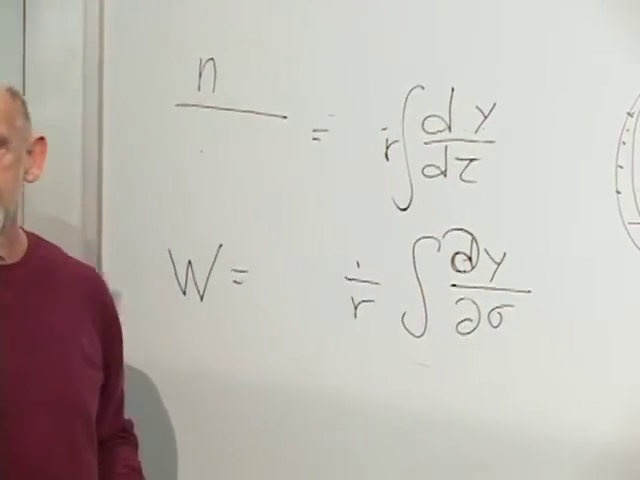
\includegraphics[width=0.72\textwidth]{lecture_10_figure_03.png}
  \medskip

  \begin{tikzpicture}[x=1cm,y=1cm,>=Latex]
    \draw[thick] (-4.0,0.3) circle (0.65);
    \draw[->,thick] (-4.55,0.58) arc (150:-145:0.65);
    \node at (-4.0,-0.65) {$w=+1$};
    \draw[thick] (-2.0,0.3) circle (0.65);
    \draw[->,thick] (-2.55,0.58) arc (150:-145:0.65);
    \node at (-2.0,-0.65) {$w=+1$};
    \node at (-3.0,0.3) {$+$};
    \draw[->,thick] (-1.0,0.3) -- (0.3,0.3);
    \draw[thick] (1.45,0.3) circle (0.78);
    \draw[thick] (1.45,0.3) circle (0.52);
    \draw[->,thick] (0.81,0.74) arc (145:-145:0.78);
    \node at (1.45,-0.78) {$w=+2$};
  \end{tikzpicture}
  \caption{纏繞方向相同的弦可以重新接合，形成纏繞兩次的弦。連通性雖有改變，總纏繞數仍為二。}
  \lectureframe{00:16:40}
  \label{fig:l10-same-winding}
\end{figure}

這項區別在所有允許的過程中都成立。總纏繞數為一百，可以由一根纏繞一百次的弦承載，也可以由兩根各纏繞五十次的弦，或一百根各纏繞一次的弦承載。弦可以在這些情況之間分裂與接合，但帶符號的總和始終是一百。我們以 \(w\in\mathbb Z\) 表示。

\section{動量模態與纏繞模態}

光有守恆還不足以構成對偶性。接下來要比較能量。沿緊緻圓方向運動的態具有量子化動量
\begin{equation}
  p_Y=\frac{n}{R},
  \qquad n\in\mathbb Z.
  \label{eq:l10-compact-momentum}
\end{equation}
若可忽略該態的其他質量貢獻，緊緻方向的運動會貢獻 \(E_{\rm mom}=|n|/R\)。正、負的 \(n\) 代表相反的運動方向，但能量仍為正。

\begin{figure}[H]
  \centering
  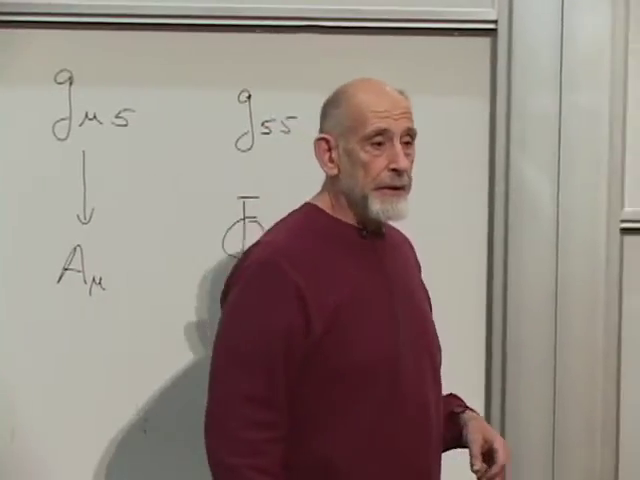
\includegraphics[width=0.72\textwidth]{lecture_10_figure_04.png}
  \caption{板書上的緊緻方向動量量子數。本講以示意方式將動量寫成緊緻方向速度的積分。}
  \lectureframe{00:21:30}
  \label{fig:l10-compact-momentum-board}
\end{figure}

纏繞 \(|w|\) 次的弦，其長度為 \(2\pi |w|R\)。基本弦張力為
\begin{equation}
  T_{\rm F}=\frac{1}{2\pi\alpha'},
\end{equation}
因此纏繞能量為
\begin{equation}
  E_{\rm wind}=T_{\rm F}(2\pi |w|R)
  =\frac{|w|R}{\alpha'}.
  \label{eq:l10-winding-energy}
\end{equation}
在本講採用的單位 \(\alpha'=1\) 下，能量就是 \(E_{\rm wind}=|w|R\)。

半徑變化時，兩座能譜塔的行為恰好相反。當 \(R\gg
\sqrt{\alpha'}\) 時，動量能級間距小，纏繞能級間距大。當 \(R\ll\sqrt{\alpha'}\) 時，動量能級間距大，纏繞能級間距小。

\begin{figure}[H]
  \centering
  \begin{minipage}[t]{0.48\textwidth}
    \centering
    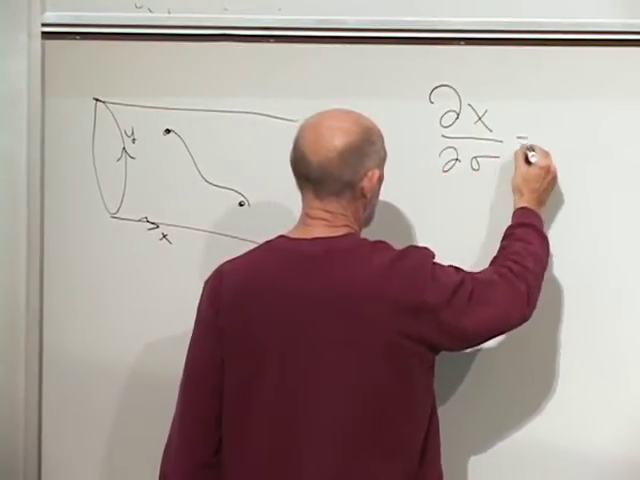
\includegraphics[width=\linewidth]{lecture_10_figure_05.png}
    \par\smallskip
    \textit{緊緻半徑較大。}
  \end{minipage}\hfill
  \begin{minipage}[t]{0.48\textwidth}
    \centering
    \includegraphics[width=\linewidth]{lecture_10_figure_06.png}
    \par\smallskip
    \textit{緊緻半徑較小。}
  \end{minipage}
  \caption{板書比較的兩種能譜。半徑取倒數後，稀疏與密集的能譜塔互換角色。}
  \lectureframe{00:25:30--00:26:00}
  \label{fig:l10-dual-spectra-board}
\end{figure}

清楚的示意圖如下
\begin{figure}[H]
  \centering
  \begin{adjustbox}{max width=\linewidth}
  \begin{tikzpicture}[x=1cm,y=0.74cm,>=Latex]
    \node[font=\bfseries] at (-3.6,6.2) {$R\gg\sqrt{\alpha'}$};
    \draw[->] (-5.1,0) -- (-5.1,5.5) node[above] {$E$};
    \foreach \y in {0.4,1.0,1.6,2.2,2.8,3.4,4.0,4.6}
      \draw (-5.35,\y)--(-4.85,\y);
    \node[align=center] at (-4.25,5.15) {momentum\\dense};
    \draw[->] (-2.2,0) -- (-2.2,5.5) node[above] {$E$};
    \foreach \y in {0.4,2.4,4.4}
      \draw (-2.45,\y)--(-1.95,\y);
    \node[align=center] at (-1.35,5.15) {winding\\sparse};

    \node[font=\bfseries] at (3.6,6.2) {$R\ll\sqrt{\alpha'}$};
    \draw[->] (2.2,0) -- (2.2,5.5) node[above] {$E$};
    \foreach \y in {0.4,2.4,4.4}
      \draw (1.95,\y)--(2.45,\y);
    \node[align=center] at (3.05,5.15) {momentum\\sparse};
    \draw[->] (5.1,0) -- (5.1,5.5) node[above] {$E$};
    \foreach \y in {0.4,1.0,1.6,2.2,2.8,3.4,4.0,4.6}
      \draw (4.85,\y)--(5.35,\y);
    \node[align=center] at (5.95,5.15) {winding\\dense};
  \end{tikzpicture}
  \end{adjustbox}
  \caption{能級間距論證的重建。動量與纏繞數連同 \(R\leftrightarrow\alpha'/R\) 一起互換時，完整的弦譜保持不變。}
  \label{fig:l10-dual-spectra-redraw}
\end{figure}

假設有人拿到其中一種能譜，卻不知道它是如何形成的。間距較小的能譜塔，究竟代表大圓上的動量，還是小圓上的纏繞？單憑能譜無法判斷。弦理論提出更強的主張：散射振幅也無法判別這兩種描述。它們在
\begin{equation}
  n\longleftrightarrow w,
  \qquad
  R\longleftrightarrow \widetilde R=\frac{\alpha'}{R}.
  \label{eq:l10-radius-duality}
\end{equation}
之下完全等價。自對偶半徑為
\begin{equation}
  R=\sqrt{\alpha'},
  \label{eq:l10-self-dual-radius}
\end{equation}
也就是本講單位下的 \(R=1\)。在這個半徑處，額外的態可能變成無質量態，規範對稱性也會增強。

\begin{classroomqa}
\audiencequestion{纏繞只是一種重寫能譜的數學技巧嗎？\lecturetimestamp{00:27:33}}
\lecturerresponse{不是。纏繞標記閉弦希爾伯特空間中的真實扇區，而這些扇區也參與交互作用。``對偶''意指動量描述與纏繞描述是同一物理的不同座標，而不是其中一個扇區只是另一個扇區可有可無的助記方式。}
\end{classroomqa}

\begin{classroomqa}
\audiencequestion{是否有一個半徑在對偶作用下映射到自身？
\lecturetimestamp{00:27:58}}
\lecturerresponse{有。自對偶半徑為 \(R=\sqrt{\alpha'}\)，以板書採用的單位表示則是 \(R=1\)。兩座能譜塔在此相遇，能譜也具有增強的對稱性。}
\end{classroomqa}

\section{對偶性的世界面表述}

能譜的論證頗具啟發性，但世界面上的描述能更精確地說明這種交換。在共形規範下，與 \(Y\) 共軛的動量正比於 \(\partial_\tau Y\)。因此，總緊緻方向動量的形式為
\begin{equation}
  P_Y=\frac{1}{2\pi\alpha'}
      \int_0^{2\pi}d\sigma\,\partial_\tau Y.
  \label{eq:l10-worldsheet-momentum}
\end{equation}
纏繞數則為
\begin{equation}
  w=\frac{1}{2\pi R}
      \int_0^{2\pi}d\sigma\,\partial_\sigma Y
   =\frac{Y(2\pi)-Y(0)}{2\pi R}.
  \label{eq:l10-worldsheet-winding}
\end{equation}

\begin{classroomqa}
\audiencequestion{為什麼沿閉弦積分導數不會得到零？\lecturetimestamp{00:32:33}}
\lecturerresponse{因為 \(Y\) 是週期性的靶空間座標，並非定義在 \(\sigma\) 圓上的單值實函數。世界面上的點 \(\sigma=2\pi\) 與 \(\sigma=0\) 是同一點，但將嵌入映射提升到覆蓋直線後，座標會改變 \(2\pi wR\)。對 \(\partial_\sigma Y\) 積分量度的正是這個位移。}
\end{classroomqa}

\begin{figure}[H]
  \centering
  \includegraphics[width=0.76\textwidth]{lecture_10_figure_07.png}
  \caption{板書完成兩行推導後得到的動量與纏繞數積分。本講採用的規範化略去了共同因子 \(2\pi\) 與 \(\alpha'\)。}
  \lectureframe{00:33:25}
  \label{fig:l10-momentum-winding-integrals}
\end{figure}

對於纏繞一圈的弦，
\begin{equation}
  Y(\tau,\sigma+2\pi)=Y(\tau,\sigma)+2\pi R.
\end{equation}
纏繞數為 \(w\) 時，右側的位移為 \(2\pi wR\)。因此，方程式 \eqref{eq:l10-worldsheet-winding} 會精確計數纏繞數。這是板書簡寫 \(w\sim R^{-1}\int
d\sigma\,\partial_\sigma Y\) 的精確表述。

因此，T 對偶在世界面上的表述為
\begin{equation}
  \partial_\tau Y\longleftrightarrow
  \partial_\sigma \widetilde Y,
  \qquad
  \partial_\sigma Y\longleftrightarrow
  \partial_\tau \widetilde Y,
  \label{eq:l10-derivative-duality}
\end{equation}
也就是說，\(Y\) 中的動量會變成對偶座標 \(\widetilde Y\) 中的纏繞，反之亦然。

\begin{classroomqa}
\audiencequestion{這是否表示世界面座標 \(\tau\) 和 \(\sigma\) 本身彼此相關或互換？
\lecturetimestamp{00:34:39}}
\lecturerresponse{不是。T 對偶會映射解，並交換緊緻靶空間座標的特定導數；它不會把世界面的時間座標與空間座標視為相同。}
\end{classroomqa}

\section{為什麼無法排除纏繞態}

有人或許會問：既然弦也可以處於未纏繞態，為什麼還會出現纏繞態？弦不會依照偏好選擇狀態。碰撞所提供的能量會拉伸弦。能量足夠高、形變嚴重的弦，可能重新接合成兩根纏繞方向相反的弦。它們的總纏繞數仍為零，但分裂後兩根弦可能彼此分離。若將其中一根送到很遠的地方，觀察者便會看到一根似乎孤立的纏繞弦。

\begin{figure}[H]
  \centering
  \includegraphics[width=0.76\textwidth]{lecture_10_figure_08.png}
  \caption{淨纏繞數為零且高度拉伸的組態；重新接合後，纏繞方向相反的弦可以由此分離。}
  \lectureframe{00:36:15}
  \label{fig:l10-winding-pair-production}
\end{figure}

能量閾值由纏繞能量決定。在大圓上，必須有很高的碰撞能量，才能將足夠長的弦沿緊緻方向拉伸。然而，能量一旦超過閾值，纏繞--反纏繞對的產生便無法禁止。這類似光子碰撞產生電子--正電子對。總電荷仍為零，但帶電粒子確實存在，而且可以彼此分離。纏繞數守恆也以相同方式運作。

這個類比不只是說法相似。緊緻方向動量與纏繞是兩種不同的荷量子數。在相應的約化描述中，同號相斥、異號相吸。因此，我們應該找出傳遞這兩種作用力的向量場。

\section{五維引力中的動量荷}

從五維引力開始。大寫指標 \(M,N\) 遍歷四個普通時空方向和緊緻的第五方向。度規分解如下：
\begin{equation}
  G_{MN}\quad\longrightarrow\quad
  \bigl\{G_{\mu\nu},\,G_{\mu5},\,G_{55}\bigr\}.
  \label{eq:l10-metric-decomposition}
\end{equation}
對稱分量 \(G_{5\mu}\) 不包含 \(G_{\mu5}\) 以外的新資訊。

\begin{figure}[H]
  \centering
  \includegraphics[width=0.74\textwidth]{lecture_10_figure_09.png}
  \caption{五維度規分量的獨立群組：\(G_{\mu\nu}\)、\(G_{\mu5}\) 與 \(G_{55}\)。}
  \lectureframe{00:44:05}
  \label{fig:l10-metric-components}
\end{figure}

從四維觀點來看，
\begin{align}
  G_{\mu\nu} &\quad\hbox{is a spacetime metric},\\
  G_{\mu5} &\equiv A_\mu\quad\hbox{is a vector field},\\
  G_{55} &\equiv e^{2\varphi}\quad\hbox{is a scalar modulus}.
  \label{eq:l10-four-dimensional-fields}
\end{align}
標量 \(\varphi\) 量度緊緻方向的尺度。它可以在普通時空中平滑變化，因此 \(\varphi\) 的波就是第五維半徑的波動。

\begin{figure}[H]
  \centering
  \includegraphics[width=0.74\textwidth]{lecture_10_figure_10.png}
  \caption{板書將 \(G_{\mu5}\) 對應為向量 \(A_\mu\)，並將 \(G_{55}\) 對應為標量 \(\Phi\)。}
  \lectureframe{00:47:40}
  \label{fig:l10-vector-and-radius-modulus}
\end{figure}

混合引力分量的來源是混合動量流。具體而言，沿第五方向的動量會成為 \(G_{\mu5}\) 的源。因此，四維觀察者會將整數 \(n\) 解讀為與 \(A_\mu\) 耦合的電荷。這就是 Kaluza--Klein 機制：在高維幾何中表現為動量的量，在低維場論中則成為電荷。

\editorialnote{本講將來自 \(G_{55}\) 的標量概略地稱為``膨脹子''。在這種約化中，它實際上是半徑模量。控制弦耦合的十維弦膨脹子是另一個場，不過改變標架或施行對偶時，低維的標量組合可能會彼此混合。}

\begin{classroomqa}
\audiencequestion{標量 \(\varphi\) 是否正比於動量整數 \(n\)？\lecturetimestamp{00:48:43}}
\lecturerresponse{不是。整數 \(n\) 標記一個量子化態，並作為電荷。標量 \(\varphi(x)\) 是決定局部緊緻化尺度的連續場。它可以隨位置改變，本身並不是整數。}
\end{classroomqa}

\section{第二個向量場與纏繞荷}

纏繞也具有類似電荷的性質，但它不能以相同方式耦合到同一個向量場。要找出第二個向量場，可以回頭看最初的閉弦激發。閉弦有左行與右行振子模態。物理態必須滿足能級匹配條件：左行與右行的總激發能級必須相同。

在玻色弦理論中，未激發態是快子。只含一個左行或右行振子的態不符合能級匹配條件。因此，第一個允許的無質量態必須同時包含兩種振子，各一個：
\begin{equation}
  \alpha_{-1}^{I}\widetilde\alpha_{-1}^{J}\ket{0;k}.
  \label{eq:l10-first-massless-state}
\end{equation}
指標 \(I,J\) 遍歷橫向空間方向，包括緊緻方向。若一個指標對應普通方向，另一個則是 \(5\)，便會有兩種類似向量的振子態：
\begin{equation}
  \alpha_{-1}^{\mu}\widetilde\alpha_{-1}^{5}\ket{0;k},
  \qquad
  \alpha_{-1}^{5}\widetilde\alpha_{-1}^{\mu}\ket{0;k}.
  \label{eq:l10-two-vector-states}
\end{equation}

\begin{figure}[H]
  \centering
  \includegraphics[width=0.76\textwidth]{lecture_10_figure_11.png}
  \caption{當其中一個極化方向沿著緊緻方向時，兩種左--右振子排列會形成四維向量態。}
  \lectureframe{00:58:20}
  \label{fig:l10-two-vector-states-board}
\end{figure}

它們的對稱組合與反對稱組合分別屬於不同的時空場：
\begin{align}
  \alpha_{-1}^{(\mu}\widetilde\alpha_{-1}^{5)}\ket{0;k}
    &\longleftrightarrow G_{\mu5},\\
  \alpha_{-1}^{[\mu}\widetilde\alpha_{-1}^{5]}\ket{0;k}
    &\longleftrightarrow B_{\mu5}.
  \label{eq:l10-g-and-b-vectors}
\end{align}
前者是以緊緻動量為源的 Kaluza--Klein 向量。後者源自反對稱的 Kalb--Ramond 場，並以弦纏繞為源。因此，約化後的理論包含兩個類似光子的場，分別對應兩種荷扇區。

若兩個振子指標都指向緊緻方向，該態就是與緊緻化模量相關的標量。若兩者都指向普通的橫向方向，對稱無跡部分就是引力子，反對稱部分是 \(B_{\mu\nu}\)，而跡則對應一個標量扇區。

\begin{classroomqa}
\audiencequestion{這些態中，哪個是單態，哪個是三重態？\lecturetimestamp{01:00:21}}
\lecturerresponse{在此採用這種分類並無助益。兩種混合態都以四維向量的形式變換。將它們相加與相減，可以分離出對稱的度規極化與反對稱的 \(B\) 場極化。具有兩個緊緻方向指標的態則是四維標量。}
\end{classroomqa}

休息前整理出的完整對應關係如下：
\begin{equation}
  \boxed{
  \begin{gathered}
    n\leftrightarrow w,
    \qquad
    R\leftrightarrow\dfrac{\alpha'}{R},\\
    \partial_\tau Y\leftrightarrow\partial_\sigma\widetilde Y,
    \qquad
    G_{\mu5}\leftrightarrow B_{\mu5}.
  \end{gathered}}
  \label{eq:l10-complete-t-duality-map}
\end{equation}

\begin{figure}[H]
  \centering
  \includegraphics[width=0.72\textwidth]{lecture_10_figure_12.png}
  \caption{板書總結了 T 對偶的對應關係：動量與纏繞、半徑與倒數半徑、世界面導數，以及兩個向量場都會互換。講者將最後一行部分遮住，因此我們在方程式 \eqref{eq:l10-complete-t-duality-map} 中明確列出該行。}
  \lectureframe{01:02:20}
  \label{fig:l10-t-duality-map-board}
\end{figure}

不應將這項構造誤解為：上述每個場都已在觀測到的粒子譜中找到對應粒子。就目前而言，這只是緊緻化弦理論的一項數學結果。雖然有許多方案嘗試將這些結構與現象學連結起來，但這不是本講要處理的問題。

\section{開弦帶來新的問題}

休息後，我們重新從開弦談起。閉弦沒有端點，纏繞便無法從端點滑脫，因此可以穩定地纏繞。開弦有端點，因而沒有類似的拓撲保護纏繞數。然而，T 對偶是理論的精確對稱性。這項對稱性會如何作用於開弦？

對於自由運動的端點，弦作用量的變分會導出 Neumann 邊界條件。在簡單的 \((X,Y)\) 幾何中，
\begin{equation}
  \left.\partial_\sigma X\right|_{\partial\Sigma}=0,
  \qquad
  \left.\partial_\sigma Y\right|_{\partial\Sigma}=0.
  \label{eq:l10-neumann-boundary}
\end{equation}
力學圖像很直觀。把弦視為由無數個愈來愈小的質量元串成的鏈。若末端質量元受到非零的切向力，當它的質量趨近於零時，加速度便會發散。因此，自由端點會自行調整，直到端點的合張力為零。也可以由人固定端點並施加所需的力，但如此一來，端點便不再是自由的。

\begin{figure}[H]
  \centering
  \includegraphics[width=0.76\textwidth]{lecture_10_figure_13.png}
  \caption{開弦及其完整的 Neumann 端點條件：\(\partial_\sigma X=\partial_\sigma Y=0\)。}
  \lectureframe{01:09:20}
  \label{fig:l10-neumann-board}
\end{figure}

現在只對緊緻座標 \(Y\) 施行對偶變換。非緊緻座標 \(X\) 保持不變。方程式 \eqref{eq:l10-derivative-duality} 會將第二個 Neumann 條件轉換為
\begin{equation}
  \left.\partial_\tau\widetilde Y\right|_{\partial\Sigma}=0.
  \label{eq:l10-dirichlet-time-derivative}
\end{equation}
因此，端點在對偶緊緻方向上的位置不隨時間改變：
\begin{equation}
  \left.\widetilde Y\right|_{\partial\Sigma}=Y_0.
  \label{eq:l10-dirichlet-boundary}
\end{equation}
這就是 Dirichlet 邊界條件。

\begin{figure}[H]
  \centering
  \includegraphics[width=0.76\textwidth]{lecture_10_figure_14.png}
  \medskip

  \begin{adjustbox}{max width=\linewidth}
  \begin{tikzpicture}[x=1cm,y=1cm,>=Latex]
    \node[align=center] at (-3.5,0.8)
      {Neumann\\\(\left.\partial_\sigma Y\right|_{\partial\Sigma}=0\)};
    \draw[->,thick] (-1.7,0.8) -- (1.3,0.8)
      node[midway,above] {$T_Y$};
    \node[align=center] at (3.4,0.8)
      {Dirichlet\\\(\left.\partial_\tau\widetilde Y\right|_{\partial\Sigma}=0\)};
    \node[align=center] at (3.4,-0.5)
      {\(\widetilde Y(\tau)=Y_0\) at each endpoint};
  \end{tikzpicture}
  \end{adjustbox}
  \caption{板書上已完成的對偶端點條件，以及對其邏輯的清楚重建。T 對偶會將緊緻方向上的自由運動轉換為端點在對偶方向上的固定位置。}
  \lectureframe{01:12:35}
  \label{fig:l10-neumann-to-dirichlet}
\end{figure}

\begin{classroomqa}
\audiencequestion{為什麼對偶條件表示端點是固定的？\lecturetimestamp{01:12:39}}
\lecturerresponse{因為 \(\partial_\tau\widetilde Y=0\) 表示端點在對偶方向上的速度為零。無論端點起初位於 \(\widetilde Y\) 的哪個位置，它都會停留在該處。端點沿未施行對偶變換之方向的座標仍可自由變動。}
\end{classroomqa}

\section{固定端點的物體是 D 膜}

若端點固定，就必須有某種物體能將它留在原處。因此，精確的 T 對偶要求理論中存在一種可供開弦終止其上的新物體，也就是 D 膜。字母 \(D\) 代表 Dirichlet，並非該物體的維度。講座中提到一段歷史掌故：這些物體或許可以 Joseph Polchinski 命名，因為他的分析明確揭示了它們的動力學角色；不過，既有術語``p 膜''使 Dirichlet 成為自然的名稱。

一個 \(p\) 膜有 \(p\) 個空間維度。弦是一膜，膜是二膜，延展的三維物體則是三膜。D\(p\) 膜是一種 \(p\) 膜，基本弦端點在垂直於膜的方向上滿足 Dirichlet 條件，在沿著膜的方向上則滿足 Neumann 條件。

對偶論證並未指定 \(Y_0\) 的特定值，因此 D 膜不可能是釘在宇宙某個特定位置上的剛性固定物。它必須能夠移動。相對論也不允許絕對剛性的延展物體，因此 D 膜可以振動、彎曲。板書畫出的平坦膜只是其平衡組態，並非對其動力學的限制。

\begin{classroomqa}
\audiencequestion{開弦的兩個端點必須位於對偶座標相同的固定位置嗎？\lecturetimestamp{01:14:55}}
\lecturerresponse{不一定。兩個端點可以位於同一張 D 膜上，此時它們共享該膜在垂直方向上的位置；也可以分別位於兩張位置不同的 D 膜上，弦便會在兩膜之間伸展。膜本身也可能振動、彎曲，因此端點所在的軌跡不必始終是完全平坦的平面。}
\end{classroomqa}

\section{計算 D 膜的維度}

十維超弦理論有九個空間維度。假設 T 對偶在一個空間方向上施加 Dirichlet 條件，端點在其餘八個方向上仍可自由移動，因此其允許所在的位置構成一張八維 D8 膜。每增加一個獨立的 Dirichlet 條件，端點可移動的方向便少一個。若有 \(k\) 個空間座標被固定，則
\begin{equation}
  p=9-k.
  \label{eq:l10-dp-counting}
\end{equation}

桌面提供了同一種維度計數的三維例子。固定垂直座標後，指尖仍可在二維桌面上移動；再固定一個座標後，指尖便只能沿著一條線移動；三個座標全都固定時，指尖就被限制在一個點上。

\begin{figure}[H]
  \centering
  \begin{adjustbox}{max width=\linewidth}
  \begin{tikzpicture}[x=1.05cm,y=1cm,>=Latex]
    \draw[fill=blue!8] (-5.5,-0.7) -- (-2.5,-0.7) -- (-1.7,0.2)
      -- (-4.7,0.2) -- cycle;
    \node at (-3.6,-1.15) {one constraint: sheet};
    \draw[very thick,blue!60!black] (-0.9,-0.25) -- (1.3,-0.25);
    \node at (0.2,-1.15) {two constraints: line};
    \fill[blue!70!black] (4.1,-0.25) circle (0.09);
    \node at (4.1,-1.15) {three constraints: point};
    \draw[->] (-1.45,0.95) -- (-0.75,0.95);
    \draw[->] (2.25,0.95) -- (2.95,0.95);
    \node at (0.35,1.35) {each Dirichlet condition lowers \(p\) by one};
  \end{tikzpicture}
  \end{adjustbox}
  \caption{在桌面上說明維度計數的論證。D\(p\) 膜是端點仍能自由移動的所在位置。}
  \label{fig:l10-dp-counting-redraw}
\end{figure}

反覆施行對偶變換，可以生成 D8 膜、D7 膜、D6 膜，依此類推，直到空間中呈點狀的 D0 膜。若沒有任何空間方向受到固定，D9 膜便遍布全部九個空間維度，普通開弦也能在各處自由移動。講座中簡短提到 D\((-1)\) 膜；這類膜局域於歐幾里得時空中，表現為瞬子，而非隨時間傳播的普通粒子。

\editorialnote{這個維度階梯描述的是合併來看時的 II 型理論。穩定的 BPS D\(p\) 膜在 IIA 型理論中具有偶數個 \(p\)，在 IIB 型理論中則具有奇數個 \(p\)。沿一個圓施行 T 對偶會使 \(p\) 改變一，並同時將 IIA 型與 IIB 型理論互換。}

\begin{classroomqa}
\audiencequestion{如果只有六個維度是緊緻的，計算維度時是否應該從六開始扣除，而不是從九開始？\lecturetimestamp{01:20:49}}
\lecturerresponse{這個基本推導是在緊緻方向上施行 T 對偶；當原本的圓縮到任意小時，其對偶圓便會擴大到任意大。在這個極限下，對偶圓實際上成為非緊緻方向。因此，所得的膜可以沿著在可及尺度下看似非緊緻的方向延伸，也可以垂直於這類方向。維度 \(p\) 計算的是沿著膜的所有空間方向，而不只是在某項推導中使用的緊緻方向。}
\end{classroomqa}

D0 膜是一種新型粒子。開弦可以從一張 D0 膜延伸至另一張 D0 膜，可以返回同一張 D 膜，也可以朝非常遙遠的膜延伸。若弦真的延伸到空間無窮遠處，其長度便是無限大，能量也因此無限大；所以在物理上有用的情況，是讓弦的另一端連接到另一個物體上。

下一個情形是 D1-膜。它本身具有弦狀，但不是我們一開始討論的基本弦。它可以彎曲，也可以閉合成環；基本弦則可以終止於其上。它的張力隨弦耦合常數變化的方式不同：
\begin{equation}
  T_{\rm D1}=\frac{1}{2\pi\alpha' g_s},
  \qquad
  T_{\rm F1}=\frac{1}{2\pi\alpha'}.
  \label{eq:l10-dstring-tension}
\end{equation}
在弱耦合 \(g_s\ll1\) 下，D 弦比基本弦重得多，這也解釋了它為何一開始會像一個質量很大的錨。

\begin{figure}[H]
  \centering
  \includegraphics[width=0.76\textwidth]{lecture_10_figure_15.png}
  \caption{黑板上的 D1-膜：一種可彎曲的一維物體，與可終止於其上的基本弦不同。}
  \lectureframe{01:24:20}
  \label{fig:l10-d1-brane}
\end{figure}

\begin{classroomqa}
\audiencequestion{T 對偶也作用於 D 膜嗎？\lecturetimestamp{01:25:35}}
\lecturerresponse{會。沿著 D\(p\)-膜平行方向進行 T 對偶，會使其維度降為 D\((p-1)\)；沿著垂直方向進行 T 對偶，則會使其維度升為 D\((p+1)\)。膜也是對偶對應的一部分，並非在對偶作用下保持不變的外部支撐物。}
\end{classroomqa}

\begin{classroomqa}
\audiencequestion{沿著膜的方向仍然可以是緊緻的嗎？
\lecturetimestamp{01:27:25}}
\lecturerresponse{可以。``沿膜方向''與``緊緻''回答的是不同問題。一個方向可以沿著膜，同時閉合成圓；也可以是非緊緻的。對端點而言，關鍵在於該方向上的邊界條件是諾伊曼型還是狄利克雷型。}
\end{classroomqa}

D2-膜是一張類似薄片的膜。D3-膜有三個空間維度。在真正的高維時空中，D3-膜是三維子空間，而非整個空間；即使受限於膜上的觀測者，仍可能將它視為自身完整的空間世界。

\begin{figure}[H]
  \centering
  \includegraphics[width=0.76\textwidth]{lecture_10_figure_16.png}
  \caption{畫成薄片的 D2-膜，弦端點可以在其上移動。}
  \lectureframe{01:27:55}
  \label{fig:l10-d2-brane}
\end{figure}

這裡給出的推導刻意只作概略說明。單憑它本身，還不能證明弦理論描述了自然界。然而，在弦理論內部，有許多一致性檢驗：對偶性、量子計算和數學結果都指向 D 膜是真正的動力學物體。

\section{膜上的開弦成為場}

取一張除此之外空無一物的 D2-膜，並在其上放置短開弦。每個端點都受限於膜面，因此整個低能激發會沿著膜面移動。兩條有向弦若相鄰端點的箭頭相容，就可以接合；接合後的弦之後還可以再次分裂。若將這些過程視為粒子歷史，它們就是費曼圖的頂點：兩個粒子進入，中間有一個激發傳播，接著兩個粒子出來。

\begin{figure}[H]
  \centering
  \includegraphics[width=0.76\textwidth]{lecture_10_figure_17.png}
  \caption{D2-膜上的有向開弦透過相容的端點接合。在低能下，這個過程可視為膜上的場論交互作用。}
  \lectureframe{01:29:55}
  \label{fig:l10-open-strings-on-brane}
\end{figure}

在遠低於弦尺度的能量下，內部振動譜塔不會被激發。剩下的無質量開弦態，是膜世界體上的向量場。對單張膜而言，這是阿貝爾 \(U(1)\) 規範場，相當於膜上的電磁場。這個場不會在整個十維體空間中傳播；它的量子是開弦，而弦的端點使它們受限於膜上。

\section{膜堆疊產生非阿貝爾色荷}

現在把數張平行膜放在彼此附近。以三張膜為例，分別標記為紅、綠、藍。一條有向弦的兩個端點各有一個標籤，且標籤有序：例如，它可以從紅膜延伸到綠膜、從綠膜延伸到藍膜，或從紅膜延伸回紅膜。對於 \(N\) 張膜，無質量開弦態可以排列成一個 \(N\times N\) 矩陣：
\begin{equation}
  A_\mu{}^{i}{}_{j},
  \qquad i,j=1,\ldots,N.
  \label{eq:l10-chan-paton-matrix}
\end{equation}
這些就是 --Chan–Paton 標籤，對應一個 \(U(N)\) 規範理論。

\begin{figure}[H]
  \centering
  \includegraphics[width=0.76\textwidth]{lecture_10_figure_18.png}
  \medskip

  \begin{adjustbox}{max width=\linewidth}
  \begin{tikzpicture}[x=1cm,y=1cm,>=Latex]
    \draw[very thick,red!70!black] (-4.8,2.0)--(4.8,2.0);
    \draw[very thick,green!55!black] (-4.8,0.8)--(4.8,0.8);
    \draw[very thick,blue!70!black] (-4.8,-0.4)--(4.8,-0.4);
    \node[left] at (-4.8,2.0) {Red};
    \node[left] at (-4.8,0.8) {Green};
    \node[left] at (-4.8,-0.4) {Blue};
    \draw[->,thick] (-3.4,2.0) .. controls (-2.8,1.35) and (-2.3,1.15)
      .. (-1.7,0.8);
    \node at (-2.7,1.05) {$R\!G$};
    \draw[->,thick] (-0.6,0.8) .. controls (0.0,0.25) and (0.6,-0.05)
      .. (1.2,-0.4);
    \node at (0.1,0.0) {$G\!B$};
    \draw[->,thick] (2.1,2.0) .. controls (2.9,2.55) and (3.8,2.55)
      .. (4.3,2.0);
    \node at (3.2,2.65) {$R\!R$};
  \end{tikzpicture}
  \end{adjustbox}
  \caption{黑板上的三張平行膜，以及對膜間弦所帶有序端點標籤的清楚重構。}
  \lectureframe{01:33:15}
  \label{fig:l10-three-brane-stack}
\end{figure}

\begin{classroomqa}
\audiencequestion{一條弦真的能從紅膜延伸到綠膜，而不被其他圖線擋住嗎？\lecturetimestamp{01:35:07}}
\lecturerresponse{可以。這些膜嵌入更高維空間中。黑板上的二維圖像只是投影，因此弦可以沿著垂直於投影面的方向，繞過另一條投影線。}
\end{classroomqa}

\begin{classroomqa}
\audiencequestion{紅--綠弦必須與綠--藍弦接合，才能成為紅--藍弦嗎？\lecturetimestamp{01:35:39}}
\lecturerresponse{這是基本的局部接合規則。相容的端點相遇後，兩段弦接合成一條弦，未接合的端點則保留紅、藍標籤。更複雜的過程可以透過重複相同的操作構成。}
\end{classroomqa}

接合規則就是幾何化的矩陣乘法。紅--綠弦可以與綠--藍弦接合，因為兩條弦的綠色端點彼此相容。結果是一條紅--藍弦：
\begin{equation}
  (R,G)\circ(G,B)\longrightarrow(R,B).
  \label{eq:l10-color-composition}
\end{equation}
重複出現的指標在接合處相連，並在內部消去。這與 Yang--–Mills 交互作用頂點上的指標結構相同。

\begin{figure}[H]
  \centering
  \includegraphics[width=0.76\textwidth]{lecture_10_figure_19.png}
  \caption{堆疊膜上的開弦接合。端點取向確保其組合方式與非阿貝爾規範場採用的有序指標組合相同。}
  \lectureframe{01:36:30}
  \label{fig:l10-color-joining-board}
\end{figure}

對於三張重合的膜，完整的開弦規範群是 \(U(3)\)，共有九種向量態。其代數可分解為
\begin{equation}
  \mathfrak u(3)=\mathfrak{su}(3)\oplus\mathfrak u(1).
  \label{eq:l10-u3-decomposition}
\end{equation}
八個無跡組合具有 QCD 膠子的色結構，而對角的質心 \(U(1)\) 則是另一個獨立的阿貝爾場。

\editorialnote{講座把九種色對組合中的一種描述成可以脫離並消失，於是留下八個膠子。精確地說，三張重合膜組成的堆疊給出 \(U(3)\)，而不只是 \(SU(3)\)。要得到 QCD 八重態，必須分離、投影掉或以其他方式解耦對角的 \(U(1)\)。講座中的圖像確實有助於理解有序色指標，但並未完整推導出 QCD。}

類夸克物質只帶有一個色指標。在膜的圖像中，它由一條弦表示，弦的一個端點位於色膜堆疊上，另一個端點則位於另一張遙遠的膜上。相對於色膜堆疊而言，只有一端顯示出色標籤。反轉弦的取向，就得到反粒子。若一條類夸克弦與一條類反夸克弦的端點相容，兩者便可以接合並離開色膜堆疊；兩條取向相同的類夸克弦則無法以這種方式湮滅。

由此得到的低能理論通常是超對稱 Yang--–Mills 理論，附加物質則由膜及其交會方式決定。這些理論與 QCD 足夠相近，能用來闡明非阿貝爾動力學，但不會自動成為標準模型。若只有一張膜，相同的構造便化約為 \(U(1)\) 理論：短的膜--膜弦類似光子，而延伸至另一個扇區的有向弦則扮演正、負電荷的角色。

\section{D 弦終止於磁單極子}

現在的圖像中有兩種弦狀物體。原先的基本弦，也就是 F 弦，在 D3-膜上承載電通量。D1-膜，也就是 D 弦，在弱耦合下重得多。D 弦也可以終止於 D3-膜上。它的端點對世界體規範場而言不帶電，但帶有磁荷。對 D3-膜上的觀測者而言，這個端點就是磁單極子。

\begin{figure}[H]
  \centering
  \includegraphics[width=0.76\textwidth]{lecture_10_figure_20.png}
  \medskip

  \begin{adjustbox}{max width=\linewidth}
  \begin{tikzpicture}[x=1cm,y=1cm,>=Latex]
    \draw[fill=blue!7] (-3.8,-0.5)--(2.6,-0.5)--(3.6,0.35)--(-2.8,0.35)--cycle;
    \node at (2.25,-0.95) {D3-brane};
    \draw[very thick,red!70!black] (0.0,3.0)--(0.0,0.0);
    \fill[black] (0.0,0.0) circle (0.08);
    \node[right] at (0.15,2.1) {D-string};
    \foreach \a in {25,65,115,155} {
      \draw[->,blue!65!black] (0.0,0.0)--({1.25*cos(\a)},{0.65*sin(\a)});
    }
    \node[align=center] at (4.8,1.7) {magnetic flux\\on the D3 worldvolume};
    \draw[->] (3.7,1.35)--(1.05,0.45);
  \end{tikzpicture}
  \end{adjustbox}
  \caption{黑板上的端點構造及其清楚的物理解讀。一條終止於 D3-膜上的 D 弦，在世界體規範理論中呈現為磁單極子。}
  \lectureframe{01:41:30}
  \label{fig:l10-dstring-monopole}
\end{figure}

質量階層在定性上也符合預期。由於 D 弦張力帶有因子 \(1/g_s\)，在弱耦合下，其端點比一般電激發重得多。F 弦與 D 弦端點的電磁關係，是 IIB 型弦理論更廣泛對偶結構的一部分。

\begin{classroomqa}
\audiencequestion{D 弦的端點是中性的嗎？
\lecturetimestamp{01:42:19}}
\lecturerresponse{若以基本弦端點所帶的電荷來看，它是中性的，但並非完全不帶電。它帶有磁荷，因此是 D3-膜規範理論中的磁單極子。}
\end{classroomqa}

\section{這個構造主張了什麼，又沒有主張什麼}

從 T 對偶到膜的這段發展歷經數十年逐步建立，並非來自單一計算。一個最初為描述強子而提出的理論，後來成為量子重力的候選理論。接著，理論中的對偶性使 D 膜必須納入其譜中；而規範理論也以弦終止於膜上的低能動力學之姿再次出現。從這個意義上說，這門學科走了一個完整的循環。

D 膜及相關的對偶構造，已成為研究超對稱規範理論、強耦合系統，以及引力與場論之間關聯的有力工具。它們也透過規範／引力對偶，為流體和電漿模型帶來啟發。這些成果並不等於直接推導出觀測到的粒子譜。緊緻化幾何、膜組態、超對稱破缺及許多其他要素，仍須加以選定。

\begin{classroomqa}
\audiencequestion{由什麼決定要對偶化哪個緊緻維度？
\lecturetimestamp{01:44:59}}
\lecturerresponse{從數學上說，只要具備所需的對稱性，任何緊緻方向都可以進行對偶化，並可選擇最方便的描述方式。從物理上說，特定狀態中實現的膜取向與緊緻化資料，則由該狀態的歷史和動力學所決定。}
\end{classroomqa}

\begin{classroomqa}
\audiencequestion{磁單極子的構造是由哪種膜承載？
\lecturetimestamp{01:45:21}}
\lecturerresponse{規範理論所在的世界是一張 D3-膜。D 弦延伸至垂直方向，並終止於這張 D3-膜；它的端點就是膜上三個空間維度中所見的磁單極子。}
\end{classroomqa}

\begin{classroomqa}
\audiencequestion{D 弦也有取向嗎？
\lecturetimestamp{01:45:55}}
\lecturerresponse{有。反轉 D 弦的取向會使相應的電荷反號。兩種端點取向分別代表磁單極子與反磁單極子，正如基本弦端點的取向可以區分電荷正負。}
\end{classroomqa}

\begin{classroomqa}
\audiencequestion{這種簡單的環面圖像能解釋手徵粒子物理中的左--右不對稱嗎？
\lecturetimestamp{01:46:05}}
\lecturerresponse{單靠它本身不行。平坦環面對稱性太高。手徵譜需要更多結構，例如不對稱的膜交會、軌形投影，或緊緻化在合適的 Calabi--–Yau 幾何上。弦理論中確有產生手徵性的機制，但超出這個初等 T 對偶構造的範圍。}
\end{classroomqa}

我們追蹤了同一種對稱性的四種具體表現：譜的交換、世界面導數的交換、時空場的交換，最後是端點邊界條件的交換。最後一種表現最具決定性。它將數學上的等價性轉化為 D 膜的發現，也將開弦的動力學轉化為其世界體上的規範理論。到了這一步，用 Susskind 的話說，這場講座已耗盡它的時間、能量與動量。
\end{document}